%-----------------------------------------------------------------------
%  AMRITA VISHWA VIDYAPEETHAM
%  B.Tech (AI & DS) Final Year Thesis  --  October 2026
%  Multi-Agent Battery Management System for Predictive Health
%  Estimation, Thermal Regulation, and Safe Charging Control
%-----------------------------------------------------------------------
\documentclass[a4paper, 12pt]{report}

%---- Packages ---------------------------------------------------------
\usepackage[top=30mm,bottom=30mm,left=35mm,right=25mm]{geometry}
\usepackage{bold-extra}
\usepackage{amsmath,amsfonts,amssymb}
\usepackage{graphicx}
\graphicspath{{images/}}
\usepackage[english]{babel}
\usepackage[autostyle,english=american]{csquotes}
\MakeOuterQuote{"}
\usepackage{setspace}
\onehalfspacing
\usepackage{amsthm}
\usepackage{array}
\usepackage{booktabs}
\usepackage{longtable}
\usepackage{fancyhdr}
\usepackage{titletoc}
\usepackage{cite}
\usepackage{url}
\usepackage{caption}
\usepackage{subcaption}
\usepackage{multirow}
\usepackage{xcolor}
\usepackage{siunitx}
\usepackage{microtype}
\usepackage[hidelinks]{hyperref}
\usepackage{tikz}
\usetikzlibrary{shapes.geometric,arrows.meta,positioning,fit,backgrounds}

%---- Theorem-like environments ----------------------------------------
\theoremstyle{definition}
\newtheorem{Definition}{Definition}[section]

%---- Header / footer --------------------------------------------------
\pagestyle{fancy}
\setlength{\headheight}{14pt}
\fancyhf{}
\fancyhead[L]{\small\leftmark}
\fancyhead[R]{\small\thepage}
\renewcommand{\headrulewidth}{0.4pt}

%=======================================================================
\begin{document}

%-----------------------------------------------------------------------
%  TITLE PAGE
%-----------------------------------------------------------------------
\pagenumbering{gobble}
\thispagestyle{empty}
\begin{large}
  \begin{center}
    {\Large\bfseries MULTI-AGENT BATTERY MANAGEMENT SYSTEM FOR
    PREDICTIVE HEALTH ESTIMATION, THERMAL REGULATION,\\
    AND SAFE CHARGING CONTROL}\\[1.3cm]
    A Thesis\\[0.1cm]
    Submitted in partial fulfilment for the Degree of\\[0.1cm]
    \textbf{BACHELOR OF TECHNOLOGY}\\[0.1cm]
    in\\[0.1cm]
    \textbf{ARTIFICIAL INTELLIGENCE AND DATA SCIENCE}\\[1.0cm]
    by\\[0.2cm]
    {\Large\bfseries WRITE STUDENT NAME (ROLL NUMBER)}\\[0.1cm]
    {\Large\bfseries WRITE STUDENT NAME (ROLL NUMBER)}\\[0.1cm]
    {\Large\bfseries WRITE STUDENT NAME (ROLL NUMBER)}\\[0.1cm]
    {\Large\bfseries WRITE STUDENT NAME (ROLL NUMBER)}\\[3.0cm]
    
\includegraphics[scale=0.8]{univA.png}\\
    \vfill
    DEPARTMENT OF ARTIFICIAL INTELLIGENCE\\
    {\Large\textbf{AMRITA VISHWA VIDYAPEETHAM}}\\
    {\large COIMBATORE CAMPUS (INDIA)}\\[0.3cm]
    October 2026
  \end{center}
\end{large}

%-----------------------------------------------------------------------
%  BONAFIDE CERTIFICATE
%-----------------------------------------------------------------------
\newpage
\begin{center}
  {\large DEPARTMENT OF ARTIFICIAL INTELLIGENCE}\\
  {\Large\textbf{AMRITA VISHWA VIDYAPEETHAM}}\\
  {\large COIMBATORE CAMPUS}\\[2.2cm]
  
\includegraphics[scale=0.8]{univA.png}\\[1.5cm]
  {\Large\textbf{BONAFIDE CERTIFICATE}}
\end{center}
\vspace{0.8cm}
\noindent This is to certify that the thesis entitled
\enquote{\textbf{Multi-Agent Battery Management System for Predictive
Health Estimation, Thermal Regulation, and Safe Charging Control}}
submitted by \textbf{Student Name, Roll No:\ldots\ldots},
\textbf{Student Name, Roll No:\ldots\ldots},
\textbf{Student Name, Roll No:\ldots\ldots} and
\textbf{Student Name, Roll No:\ldots\ldots}
for the award of the \textbf{Degree of Bachelor of Technology} under
the \textbf{Faculty of Engineering} is a bonafide record of the work
carried out by them under our guidance and supervision at
"Department of Artificial Intelligence", Amrita Vishwa Vidyapeetham,
Coimbatore Campus.\\

\vfill
Submitted for the examination held on \ldots\ldots\ldots\ldots
\vfill
\textbf{INTERNAL EXAMINER} \hspace{5cm} \textbf{EXTERNAL EXAMINER}
\vfill
\begin{center}
  \textbf{Dr.~[Thesis Advisor Name]}\\
  Thesis Advisor,\\
  Assistant / Associate Professor,\\
  Department of Artificial Intelligence,\\
  Amrita Vishwa Vidyapeetham,\\
  Coimbatore Campus, India.
\end{center}

%-----------------------------------------------------------------------
%  DECLARATION
%-----------------------------------------------------------------------
\newpage
\begin{center}
  {\large DEPARTMENT OF ARTIFICIAL INTELLIGENCE}\\
  {\Large\textbf{AMRITA VISHWA VIDYAPEETHAM}}\\
  {\large COIMBATORE CAMPUS}\\[2.5cm]
  {\large\textbf{DECLARATION}}\\[0.3cm]
\end{center}
\noindent We, \textbf{Student Name}, Reg.~No:\ldots\ldots,
\textbf{Student Name}, Reg.~No:\ldots\ldots,
\textbf{Student Name}, Reg.~No:\ldots\ldots\ and
\textbf{Student Name}, Reg.~No:\ldots\ldots\ hereby declare that
this thesis entitled
\enquote{\textbf{Multi-Agent Battery Management System for Predictive
Health Estimation, Thermal Regulation, and Safe Charging Control}}
is the record of the original work done by us under the guidance of
\textbf{Dr.~[Advisor Name]}, his/her designation, Department of
Artificial Intelligence, Amrita Vishwa Vidyapeetham, Coimbatore
Campus. To the best of our knowledge, this work has not formed the
basis for the award of any degree/diploma/associateship/fellowship or
a similar award to any candidate in any University.\\\\

\vspace{1cm}
\noindent{\bf Place: Coimbatore \hfill Signature of the Students}\\
\noindent{\bf Date:\hspace{2.5cm}}
\vfill
\begin{center}
  \large{COUNTERSIGNED}\\
\end{center}
\vspace{0.6in}
\begin{center}
  \textbf{Dr.~K.P.~Soman}\\
  Professor and Dean,\\
  Department of Artificial Intelligence,\\
  Amrita Vishwa Vidyapeetham,\\
  Coimbatore Campus, India.
\end{center}

%-----------------------------------------------------------------------
%  FRONT MATTER
%-----------------------------------------------------------------------
\clearpage
\pagenumbering{roman}
\tableofcontents

%---- Acknowledgements -------------------------------------------------
\chapter*{Acknowledgements}
\addcontentsline{toc}{chapter}{Acknowledgements}

We express our heartfelt gratitude to our thesis advisor,
\textbf{Dr.~[Advisor Name]}, whose constant guidance, insightful
critiques, and patience throughout the research process made this work
possible. We thank the Department of Artificial Intelligence, Amrita
Vishwa Vidyapeetham, for providing the computational resources and an
intellectually stimulating environment.

We are deeply indebted to the \textbf{NASA Prognostics Center of
Excellence (PCoE)} for publicly releasing the Accelerated Life Testing
battery dataset, which served as the empirical backbone of this thesis.

We also thank our families and friends for their unwavering
encouragement throughout this journey.

\vspace{1cm}
\begin{flushright}
  THE AUTHORS
\end{flushright}

\listoffigures
\addcontentsline{toc}{chapter}{List of Figures}
\listoftables
\addcontentsline{toc}{chapter}{List of Tables}

%---- Abbreviations ----------------------------------------------------
\newpage
\section*{{\huge Abbreviations}\hfill}
\addcontentsline{toc}{chapter}{\textbf{Abbreviations}}
\vspace{1.2cm}
\begin{tabular}{lll}
ALT  & -- & Accelerated Life Testing \\
BMS  & -- & Battery Management System \\
CBF  & -- & Control Barrier Function \\
CC   & -- & Constant Current \\
CV   & -- & Constant Voltage \\
DRL  & -- & Deep Reinforcement Learning \\
ECM  & -- & Equivalent Circuit Model \\
EKF  & -- & Extended Kalman Filter \\
EOL  & -- & End of Life \\
EV   & -- & Electric Vehicle \\
HEV  & -- & Hybrid Electric Vehicle \\
KM   & -- & Kaplan--Meier \\
LOPO & -- & Leave-One-Pack-Out \\
MA-BMS & -- & Multi-Agent Battery Management System \\
MAE  & -- & Mean Absolute Error \\
MARL & -- & Multi-Agent Reinforcement Learning \\
MPC  & -- & Model Predictive Control \\
NASA PCoE & -- & NASA Prognostics Center of Excellence \\
OCV  & -- & Open-Circuit Voltage \\
PID  & -- & Proportional-Integral-Derivative \\
PPO  & -- & Proximal Policy Optimisation \\
RMSE & -- & Root Mean Square Error \\
RL   & -- & Reinforcement Learning \\
RUL  & -- & Remaining Useful Life \\
SAC  & -- & Soft Actor-Critic \\
SOC  & -- & State of Charge \\
SOH  & -- & State of Health \\
SPM  & -- & Single Particle Model \\
\end{tabular}

%---- Symbols ----------------------------------------------------------
\newpage
\section*{{\huge List of Symbols}\hfill}
\addcontentsline{toc}{chapter}{\textbf{List of Symbols}}
\vspace{1.2cm}
\begin{tabular}{lll}
$Q_{\mathrm{nom}}$   & -- & Nominal cell capacity (\SI{2.45}{Ah}) \\
$R_0$                & -- & Series (ohmic) internal resistance \\
$R_0^{\mathrm{new}}$ & -- & Fresh-cell series resistance (\SI{0.034}{\ohm}) \\
$k_{R_0}$            & -- & Resistance growth coefficient per SOH unit lost \\
$C_{\mathrm{th}}$    & -- & Thermal capacitance (\SI{54.5}{J/K}) \\
$h$                  & -- & Heat transfer coefficient (\SI{0.069}{W/K}) \\
$\tau_{\mathrm{th}}$ & -- & Thermal time constant $= C_{\mathrm{th}}/h$ (\SI{791}{s}) \\
$k_T$                & -- & Temperature degradation coefficient \\
$E_a$                & -- & Activation energy (Arrhenius, \SI{4068}{K}) \\
$J$                  & -- & Composite scalar reward / objective \\
$w_t, w_d, w_e$      & -- & Dirichlet weighting of time, degradation, energy \\
SOC                  & -- & State of Charge (0--1) \\
SOH$_{\mathrm{abs}}$ & -- & Absolute State of Health $= Q/Q_{\mathrm{nom}}$ \\
$\rho$               & -- & Resistance scaling state in EKF \\
$b$                  & -- & Capacity scaling state in EKF \\
$T$                  & -- & Cell surface / electrode temperature (\si{\degreeCelsius}) \\
$T_{\mathrm{amb}}$   & -- & Ambient temperature (\si{\degreeCelsius}) \\
$I$                  & -- & Applied current (\si{A}, positive = discharge) \\
$V$                  & -- & Terminal voltage (\si{V}) \\
$V_{\mathrm{max}}$   & -- & Maximum allowable voltage (\SI{8.4}{V} for 2S pack) \\
$\Delta V_{\mathrm{margin}}$ & -- & Voltage safety margin \\
\end{tabular}

%---- Abstract ---------------------------------------------------------
\chapter*{Abstract}
\addcontentsline{toc}{chapter}{Abstract}

Lithium-ion battery packs operating under variable loading regimes
face competing operational demands: minimising charging duration,
limiting thermal excursion, preventing accelerated capacity fade, and
enforcing strict electrochemical safety boundaries. This thesis
investigates a modular \textbf{Multi-Agent Battery Management System
(MA-BMS)} evaluated against the NASA Prognostics Center of Excellence
Accelerated Life Testing (ALT) dataset comprising 26 two-cell
in-series (2S) Samsung INR18650-25R packs operating at up to 3.5C
discharge rates at ambient temperatures of 25--\SI{60}{\degreeCelsius}.

A rigorous dataset audit, spanning 4{,}918{,}193 raw telemetry
rows, establishes the empirical basis: the charging protocol is pure
CC at \SI{3.0}{A} (1.2C) with a negligible constant-voltage taper
fraction ($\leq 4\%$). The audit classifies 9 hard collapses, 5
probable protection shutoffs, 3 recommissioned packs, and 10
right-censored survivors -- finding that 10 of the 15 failure events
occur \emph{above} 0.80 SOH, which invalidates capacity-fade-only
prognostic models as early warning systems.

The simulator is calibrated from the dataset: series resistance
$R_0 = \SI{0.034}{\ohm}$ (fresh), thermal capacitance
$C_{\mathrm{th}} = \SI{54.5}{J/K}$, heat transfer coefficient
$h = \SI{0.069}{W/K}$ (thermal time constant $\tau_{\mathrm{th}} =
\SI{791}{s}$), and resistance growth $R_0(\mathrm{SOH}) = R_0^{\mathrm{new}}
(1 + k_{R_0}(1-\mathrm{SOH}))$ with $k_{R_0} \sim \mathcal{U}(1.5,
4.5)$. Thermal response during rest cooling is validated on 5{,}479
physical blocks.

The MA-BMS architecture separates charging from thermal and health
concerns via three cooperative proposer agents and a deterministic
analytical safety supervisor. A tuned single-agent policy achieves
the best composite score under 10{,}000-sample Dirichlet
weight sensitivity ($84.78\%$ best-weight share), reduces
time-to-target by $20.1\%$ versus conventional CC-CV, and incurs
zero unsafe executed steps under four-times sensor noise. The
deterministic supervisor eliminates all hard voltage and temperature
violations across seven injected fault regimes.

An interval-censored Kaplan-Meier survival analysis (endpoints A, B,
C) yields a median throughput of $630$--$833$~Ah across endpoint
definitions. A Leave-One-Pack-Out Ridge regression for RUL achieves
MAE $= 122.4$~Ah (RMSE $= 153.9$~Ah, $R^2 = 0.787$), outperforming
linear and population baselines. The study formally downgrade RQ1:
the health-cap controller does not demonstrate statistically
significant capacity-fade reduction relative to the independent
baseline, as its $R_0$-induced thermal throttling under aged packs
reduces deadline success from 93.3\% to 65.6\%.

\clearpage
\pagenumbering{arabic}
\setcounter{page}{1}

%-----------------------------------------------------------------------
%  CHAPTERS
%-----------------------------------------------------------------------
\chapter{Introduction}
\section{Background and Motivation}

The global transition towards electrified transportation, renewable
energy integration, and grid-scale storage has made the lithium-ion
battery one of the most strategically important technologies of the
twenty-first century.  Despite decades of engineering progress,
lithium-ion cells remain intrinsically fragile: their electrochemical
stability depends on maintaining terminal voltage, current, and
temperature within narrow operating windows.  Violations of these
limits---even momentary---accelerate solid-electrolyte interphase
(SEI) growth, lithium plating, mechanical particle cracking, and, in
severe cases, thermal runaway \cite{vetter2005ageing}.

A \emph{Battery Management System} (BMS) is the firmware and hardware
subsystem responsible for enforcing these limits in real time while
simultaneously optimising competing objectives: charging as fast as
possible (to minimise user inconvenience), maintaining cell
temperature within acceptable bounds (to extend cycle life), limiting
degradation-inducing high-current and high-SOC exposure (to maximise
capacity retention), and guaranteeing hard electrochemical safety
constraints (to prevent cell failure or fire).

These four objectives are fundamentally in tension.  Faster charging
requires higher current, which generates more Joule heat and
accelerates resistance-mediated degradation.  Aggressive active
cooling consumes additional energy.  A purely safety-focused strategy
derate current so conservatively that deadline requirements are
missed.  Classical constant-current / constant-voltage (CC-CV)
protocols resolve this tension through fixed schedules, ignoring both
real-time cell state and the substantial cell-to-cell variability that
emerges as packs age.

\section{Problem Statement}

Modern BMS research has explored three broad paradigms: rule-based
classical control (CC-CV, multi-stage constant current), Model
Predictive Control (MPC) using Equivalent Circuit Models or
electrochemical models, and single-agent Deep Reinforcement Learning
(DRL) \cite{park2020fastcharging, torchio2016lionsimba, wu2021dqn}.
Each suffers from a fundamental shortcoming.

\begin{enumerate}
  \item \textbf{Classical methods} are static: they cannot adapt to
  individual cell ageing trajectories or dynamic thermal environments.

  \item \textbf{MPC methods} suffer from computational overhead and
  critical sensitivity to model mismatch: as $R_0$ rises with
  degradation, MPC controllers calibrated on fresh cells generate
  systematically incorrect voltage predictions.

  \item \textbf{Single-agent DRL} entangles all objectives into a
  single scalarised reward.  The resulting policy is highly sensitive
  to objective weight selection; small weight perturbations can cause
  policy collapse---catastrophically missing deadlines or violating
  soft voltage boundaries \cite{achiam2017cpo}.
\end{enumerate}

A fourth gap, common to all paradigms, is the absence of
\emph{deterministic} hard safety guarantees: purely neural or
optimisation-based policies have no provable mechanism to
prevent unsafe actions when sensors are faulty or cell parameters
deviate from nominal.

\section{Research Questions}

This thesis addresses four specific research questions derived from
the identified gaps:

\begin{description}
  \item[RQ1.] Does a dedicated health-cap agent, limiting peak current
  to reduce degradation-inducing high-current exposure, produce
  statistically significant capacity-fade reduction compared to an
  independent-deadline baseline under realistic aged-resistance
  variability?

  \item[RQ2.] Can a deterministic analytical safety supervisor
  maintain zero hard voltage and temperature violations across diverse
  sensor fault types (bias, dropout, stuck sensor) at multiple
  charging aggressiveness levels?

  \item[RQ3.] Does a multi-agent functional decomposition
  (with separate proposers for charging speed, thermal regulation, and
  health) outperform single-agent and conventional alternatives across
  a broad range of Dirichlet-sampled objective weights?

  \item[RQ4.] What is the empirically grounded survival distribution
  and Leave-One-Pack-Out (LOPO) RUL prediction accuracy achievable
  from the NASA PCoE ALT dataset, given proper interval-censored
  failure classification?
\end{description}

\section{Contributions}

The principal contributions of this thesis are:

\begin{enumerate}
  \item \textbf{Rigorous empirical dataset audit} of the NASA PCoE
  26-pack ALT dataset, clarifying the CC-only charging protocol
  (3.0\,A, negligible CV taper), correcting the EOL classification
  (9 hard collapses, 5 probable shutoffs, 3 recommissioned, 10
  right-censored), and demonstrating that 67\% of genuine failures
  occur above 0.80 SOH --- invalidating capacity-threshold-only
  prognostic systems.

  \item \textbf{Physics-based simulator calibration} from real
  telemetry: OCV curve, $R_0 = 0.034\,\Omega$ (fresh), thermal
  parameters ($C_\mathrm{th} = 54.5$\,J/K, $h = 0.069$\,W/K,
  $\tau_\mathrm{th} = 791$\,s), and aging-dependent
  $R_0(\mathrm{SOH})$ growth verified across 5{,}479 rest cooling
  blocks.

  \item \textbf{Four-state Adaptive EKF} with state vector
  $[{\rm SOC}, V_1, b, \rho]^\top$, reducing terminal SOC error by
  72.3\% compared to a fixed-parameter EKF and eliminating unsafe
  executed steps on the single-agent tuned policy.

  \item \textbf{MA-BMS architecture} with three cooperative proposer
  agents and a deterministic analytical safety supervisor, achieving
  zero unsafe executed steps under $4\times$ sensor noise and zero
  hard violations across all seven injected sensor fault regimes.

  \item \textbf{Dirichlet weight sensitivity analysis} over
  10{,}000 samples showing that the tuned single-agent policy holds
  an 84.78\% best-weight share, while demonstrating that all four
  methods are Pareto-nondominated, formally qualifying the ranking.

  \item \textbf{Interval-censored survival analysis} and
  Leave-One-Pack-Out RUL study, obtaining Kaplan-Meier median
  throughputs of 630--833\,Ah and Ridge MAE of 122.4\,Ah
  ($R^2 = 0.787$).
\end{enumerate}

\section{Scope and Limitations}

The scope of this work is bounded to the control and prognostics of a
single two-cell in-series pack operating under laboratory accelerated
ageing conditions.  Key limitations are:

\begin{itemize}
  \item Charge-phase current and voltage are not independently logged
  in the NASA dataset; only thermal response during charging is
  validated.  Current dynamics are inferred from the paper (pure CC
  at 3.0\,A).
  \item The RUL sample is small (10 crosser packs in regression);
  LOPO estimates have wide confidence intervals.
  \item The multi-agent coordination layer (coordinator agent) is
  designed but not benchmarked in this thesis; only single-agent and
  independent-baseline variants are fully evaluated.
\end{itemize}

\section{Thesis Organisation}

The remainder of the thesis is organised as follows.
Chapter~\ref{chap.2} reviews the relevant literature.
Chapter~\ref{chap.3} presents the dataset audit.
Chapter~\ref{chap.4} describes simulator calibration and thermal
validation.  Chapter~\ref{chap.5} details the MA-BMS architecture and
EKF design.  Chapter~\ref{chap.6} presents the controller
benchmarking and robustness results.  Chapter~\ref{chap.7} covers
survival analysis and RUL prediction.  Chapter~8 concludes and
outlines future work.


\chapter{Literature Review}
\label{chap.2}

\section{Introduction}

Battery management for lithium-ion cells sits at the convergence of
electrochemical modelling, control theory, state estimation, and
machine learning.  This chapter surveys the four principal paradigms
in chronological and thematic order, identifies the key gaps that
motivate the present work, and maps each contribution of this thesis
to the gap it addresses.

\section{Classical Charging Protocols}

The industry-standard CC-CV protocol applies a constant current
until the terminal voltage reaches the cut-off threshold, then holds
the voltage constant while the current decays to a minimum cut-off
\cite{bloom2001accelerated}.  Variants such as multi-stage constant
current (MCC) and pulse charging have been proposed to reduce
polarisation losses and thermal excursions
\cite{purushothaman2006multistage}.

The fundamental limitation of all classical protocols is their
open-loop, parameter-agnostic nature.  They do not adapt to
cell-to-cell variability in internal resistance, ambient temperature,
or the degradation state of the cell.  As the series resistance
$R_0$ grows with ageing, a fixed-current protocol produces
increasingly large voltage drops, causing the CV transition to occur
at progressively lower SOC values, effectively truncating each charge
cycle.

\section{Model Predictive Control for Battery Charging}

MPC-based fast charging formulates a finite-horizon constrained
optimisation problem over an electrochemical or equivalent circuit
model of the battery \cite{torchio2016lionsimba}.  The Single
Particle Model (SPM) or Doyle-Fuller-Newman (DFN/P2D) model provides
physics-based state equations; the MPC minimises charging time
subject to internal potential and temperature constraints.

Torchio et al.~\cite{torchio2016lionsimba} demonstrated that
NMPC with a P2D model can reduce charging time by 20--30\% relative
to CC-CV while respecting lithium plating and temperature limits.
However, two critical limitations apply: (1) P2D numerical
integration carries prohibitive real-time computational cost, and
(2) the model parameters ($R_0$, diffusion coefficients, heat
generation) are assumed fixed.  As the cell ages, the growing
$R_0$ causes the MPC to underestimate voltage and overshoot
current, causing unmodelled plating at high SOC.

\section{Single-Agent Deep Reinforcement Learning}

Deep Reinforcement Learning (DRL) has been applied to battery fast
charging as a way to learn current policies directly from
simulator interactions, sidestepping the need for explicit
electrochemical models \cite{park2020fastcharging, wu2021dqn}.
Park et al.~\cite{park2020fastcharging} used a Deep Deterministic
Policy Gradient (DDPG) agent to discover optimal multi-step
current profiles in an equivalent circuit model, reporting an
improvement in charging time over MCC protocols.

The primary weakness of single-agent DRL is the \emph{objective
entanglement} problem.  The scalar reward
$R_t = -(w_t \cdot \Delta t + w_d \cdot D_t + w_e \cdot E_t + w_v
\cdot V_{\mathrm{pen},t})$ aggregates charging time, degradation,
energy cost, and voltage violations with fixed weights.  The resulting
policy is acutely sensitive to these weight ratios: small
perturbations cause the learned policy to either sacrifice cell
health or miss charging deadlines entirely.  Wu et al.~\cite{wu2021dqn}
introduced a DQN with heuristic thermal throttling, adding a rule-based
override on top of the neural policy.  While this reduces thermal
violations, it introduces chattering instability near the threshold.

\section{Multi-Agent Reinforcement Learning in Battery Systems}

Multi-Agent Reinforcement Learning (MARL) has been applied
predominantly to multi-cell balancing in battery packs and energy
market trading for large-scale battery energy storage systems (BESS)
\cite{cao2020marl_energy, li2022marl_grid, zhang2022maddpg}.  In
these formulations, each spatial entity (cell, inverter, generator)
is assigned a dedicated agent, and agents learn cooperative or
competitive policies.

The present work differs fundamentally: rather than assigning agents
to spatial entities, we assign agents to \emph{functional control
objectives} of a single pack.  This \emph{functional decomposition}
paradigm preserves the modularity advantages of multi-agent systems
while eliminating inter-cell coupling complexity.

\section{Safe Reinforcement Learning}

Safe RL addresses the critical failure mode of neural policies: their
inability to \emph{guarantee} constraint satisfaction.  Achiam et
al.~\cite{achiam2017cpo} proposed Constrained Policy Optimisation
(CPO), adding a Lagrangian constraint on cumulative cost.  Zou et
al.~\cite{zou2023cbf} combined DDPG with a Control Barrier Function
(CBF) safety filter, projecting unsafe actions onto the safe manifold
via a real-time quadratic program.

Both approaches share a fundamental vulnerability: the safety
guarantee depends on accurate state observation.  When a temperature
sensor is stuck or biased low by $-5\,^\circ\mathrm{C}$, the observed
state appears safe while the true cell is overheating.  The CBF
constraint is then satisfied on a false observation, permitting
thermal runaway.  Our deterministic analytical supervisor addresses
this by incorporating $R_0$ margins and a thermal plausibility
residual monitor operating on model predictions, not sensor readings
alone.

\section{State and Parameter Estimation Under Ageing}

Accurate state-of-charge (SOC) and state-of-health (SOH) estimation
is essential for all BMS paradigms.  The Extended Kalman Filter (EKF)
is the canonical approach \cite{plett2004ekf}, with extensions to dual
EKF (simultaneous estimation of SOC and $R_0$) and sigma-point
variants \cite{hu2012ekf}.  Wang et al.~\cite{wang2017dual_ekf}
proposed a joint EKF for SOC--SOH estimation, improving accuracy under
degradation.

The key gap in existing literature is \emph{initialisation under
aged conditions}: estimators that initialise $\rho_0 = 1.0$ (fresh
cell assumption) for an aged cell with $R_0 \approx 1.5\times$ the
nominal value will systematically under-predict terminal voltage,
causing premature current derating and missed deadlines.  Our 4-state
EKF initialises $\rho_0 = r_0\text{\_scale}(\widehat{\mathrm{SOH}})$,
which eliminates this bias.

\section{Empirical Grounding and RUL Evaluation}

Rigorous experimental validation is the weakest link in battery
control literature.  Most DRL charging papers use synthetic ECM
simulators fitted to fresh cells, without auditing the raw
dataset for logging artefacts or charge-phase telemetry
completeness.  Studies using the NASA PCoE dataset
\cite{saha2008battery, fricke2023nasa} frequently misinterpret
the logging definitions, misclassify relay-open transient collapses
as internal short circuits, and assume all 26 packs experienced
classical capacity-fade EOL.

RUL evaluation is equally fragile: treating RUL as a standard
regression target over a small sample of fewer than 15 failures
without accounting for right-censored packs leads to severely
optimistic error estimates \cite{saxena2015remaining}.

\section{Comparative Synthesis of Related Works}

To establish a clear structural overview of where existing approaches fall
short, Table~\ref{tab:lit_comparison} evaluates representative battery
charging, management, and prognostics literature across six foundational
axes: control paradigm, multi-objective formulation, aging awareness,
safety guarantees, fault robustness, and empirical validation grounding.

\begin{table}[htbp]
  \centering
  \caption{Systematic comparison of related battery management literature against the proposed MA-BMS framework.}
  \label{tab:lit_comparison}
  \resizebox{\columnwidth}{!}{%
  \begin{tabular}{lp{2.8cm}p{3.2cm}cccp{3.5cm}}
    \toprule
    \textbf{Study / Reference} & \textbf{Control Paradigm} & \textbf{Objective Formulation} &
    \textbf{Aging ($R_0$)} & \textbf{Hard Safety} & \textbf{Fault Robust} &
    \textbf{Empirical Grounding} \\
    \midrule
    Bloom et al.~\cite{bloom2001accelerated} &
      Classical CC-CV & Single objective (time) & Static & No (heuristic) & No &
      Laboratory cycler \\
    Torchio et al.~\cite{torchio2016lionsimba} &
      Electrochemical NMPC & Constrained min-time & Static (fresh) & Partial (model-brittle) & No &
      Synthetic P2D simulation \\
    Park et al.~\cite{park2020fastcharging} &
      Single-Agent DDPG & Entangled scalar reward & Static fixed & No (soft penalty) & No &
      Synthetic ECM \\
    Wu et al.~\cite{wu2021dqn} &
      DQN + Heuristic Rule & Scalar reward + override & Static fixed & Partial (rule derating) & No &
      Synthetic ECM \\
    Zou et al.~\cite{zou2023cbf} &
      Safe DRL via CBF & Scalar reward + QP filter & Static fresh & Partial (bias-vulnerable) & No &
      Simulation only \\
    Zhang et al.~\cite{zhang2022maddpg} &
      Spatial MADDPG & Spatial cell balancing & Static & No (soft penalty) & No &
      Synthetic multi-cell \\
    Wang et al.~\cite{wang2017dual_ekf} &
      Joint Dual EKF & State estimation only & Dynamic tracking & N/A (observer only) & Partial &
      Pulsed cell tests \\
    \midrule
    \textbf{Proposed MA-BMS} &
      \textbf{Functional Multi-Agent} & \textbf{Decoupled Proposers} &
      \textbf{Adaptive $R_0(\mathrm{SOH})$} & \textbf{Yes (Analytical $I_{\mathrm{safe}}$)} &
      \textbf{Yes (Monitor)} & \textbf{NASA ALT (4.9M rows, validated} \\
    \textbf{(This Thesis)} &
      \textbf{+ Safety Supervisor} & \textbf{+ Dirichlet Tuning} &
      \textbf{$k_{R_0} \sim \mathcal{U}(1.5, 4.5)$} & \textbf{0\% hard violations} &
      \textbf{7 fault types} & \textbf{thermal cooling \& OCV)} \\
    \bottomrule
  \end{tabular}%
  }
\end{table}

\section{Summary of Gaps and Thesis Positioning}

Table~\ref{tab:lit_gaps} summarises the key gaps and their
correspondence to contributions in this thesis.

\begin{longtable}{>{\raggedright}p{4cm}
                  >{\raggedright}p{4.5cm}
                  >{\raggedright\arraybackslash}p{4cm}}
\caption{Summary of literature gaps and corresponding contributions.}
\label{tab:lit_gaps}\\
\toprule
\textbf{Gap} & \textbf{Limitation in Literature} &
\textbf{Contribution in This Thesis} \\
\midrule
\endfirsthead
\multicolumn{3}{c}{\tablename\ \thetable\ -- \textit{Continued}}\\
\toprule
\textbf{Gap} & \textbf{Limitation in Literature} &
\textbf{Contribution in This Thesis} \\
\midrule
\endhead
\bottomrule
\endfoot
Static $R_0$ in controllers &
MPC and DRL controllers calibrated on fresh cells fail under aged
resistance ($1.57\times$ growth) &
Aging-dependent $R_0(\mathrm{SOH})$ in simulator; adaptive EKF
initialisation \\[4pt]
Objective entanglement &
Single scalar reward collapses under weight perturbation &
Functional agent decomposition + Dirichlet weight sensitivity analysis
\\[4pt]
No deterministic safety guarantee &
Neural policies violate hard limits under sensor faults &
Analytical safety supervisor: 0 violations across 7 fault types \\[4pt]
Dataset audit gaps &
Misclassified EOL events; unverified charge telemetry &
Full mode audit; CC-only charging confirmed; corrected EOL labels \\[4pt]
Na\"{\i}ve RUL evaluation &
Standard regression ignores censoring and small sample &
Interval-censored Kaplan-Meier + LOPO Ridge regression \\
\end{longtable}


\chapter{Dataset Audit and Empirical Characterisation}
\label{chap.3}

\section{Dataset Overview}

The NASA Prognostics Center of Excellence (PCoE) Accelerated Life
Testing dataset \cite{fricke2023nasa} comprises 26 two-cell in-series
(2S) Samsung INR18650-25R NCA lithium-ion packs.  Each pack was cycled
continuously under accelerated discharge conditions at ambient
temperatures of 25, 40, or \SI{60}{\degreeCelsius} with discharge
C-rates of 1.5C, 2.0C, 2.5C, or 3.5C until cell failure or test
termination.  The raw telemetry totals 4{,}918{,}193 rows logged
at \SI{1}{Hz}.

The Samsung INR18650-25R cell has a rated capacity of \SI{2.5}{Ah},
a maximum voltage of \SI{4.2}{V}, a minimum voltage of \SI{2.5}{V},
and operates within a two-cell series configuration with pack
maximum voltage of \SI{8.4}{V} and minimum of \SI{5.0}{V}
\cite{samsung2015datasheet}.

\section{Column Structure and Mode Identification}

\subsection{Telemetry Columns}

The raw HDF5 files expose the following primary signals: pack terminal
voltage, pack current, cell surface temperature (thermistor on the
nickel plate at the ground connector), discharge capacity (Ah), and a
\texttt{mission\_type} flag.  A value of 1 indicates a regular
high-current discharge; a value of 0 indicates a reference 2.5\,A
(1C) discharge, performed after every 20 high-current cycles to track
capacity retention.

\subsection{Mode Audit}

Script \texttt{18\_mode\_audit.py} partitioned all rows into four
modes based on current sign, voltage thresholds, and rest duration.
Table~\ref{tab:mode_audit} summarises the block-level outcome across
all 26 packs.

\begin{table}[htbp]
  \centering
  \caption{Mode audit block summary across 26 packs.}
  \label{tab:mode_audit}
  \begin{tabular}{lrr}
    \toprule
    \textbf{Mode} & \textbf{Block count} & \textbf{Fraction (\%)} \\
    \midrule
    Discharge (regular)  & 14{,}872 & 55.3 \\
    Discharge (reference)&  1{,}890 &  7.0 \\
    Charge              &  6{,}218 & 23.1 \\
    Rest                &  3{,}920 & 14.6 \\
    \bottomrule
  \end{tabular}
\end{table}

\subsection{Charging Protocol Verification}

The charge blocks were inspected for evidence of a CV taper phase.
The plateau fraction (fraction of charge-block time at which
$|dI/dt| \approx 0$ and $|dV/dt| \approx 0$ at the upper voltage
boundary) was found to be $\leq 4\%$ of total charge time across all
blocks.  This confirms that the charging protocol is effectively
\textbf{pure CC at 3.0\,A} ($1.2\,\text{C}$ relative to rated
capacity) with negligible constant-voltage taper.

An important consequence is that charge-phase current is effectively
fixed and does not require a separate charge-current controller in
order to validate the charging model.  The charge-block temperature
rise of $A = 6.26\,^\circ\mathrm{C}$ over a typical \SI{2400}{s}
charge block is fully consistent with the simulator's thermal model
(Section~\ref{sec:thermal_val}).

\section{Throughput Accounting}

All throughput values in this thesis are expressed in cumulative Ah
of \emph{discharge} capacity.  Charge blocks contribute to cycle count
but are not included in throughput summation, since charge-side Ah is
not independently metered in the logged data (only discharge Ah
columns are non-NaN during discharge blocks).

\section{End-of-Life Classification}

\subsection{Classification Methodology}

End-of-life for this dataset is defined as \emph{abrupt loss of
usable discharge capacity}, not a classical gradual 80\% retention
threshold.  Packs were classified into the following categories based
on visual inspection of reference discharge trajectories,
charge-block terminal voltage profiles, and absolute SOH trends:

\begin{description}
  \item[\texttt{event\_strong} (9 packs):] A clear step-drop of
  $\geq 30\%$ in reference discharge Ah within one or two cycles,
  consistent with sudden internal short-circuit or separator collapse.
  Packs 02, 11, 13, 21, 22, 32, 36, 50, 52.

  \item[\texttt{event\_charger\_dead} (1 pack):] Pack 23 failed due
  to charger-side anomaly, identified via terminal charge voltage
  reaching $v_{c,\max} = -0.111\,\mathrm{V}$ in the last charge block.

  \item[\texttt{transient\_collapse} (1 pack):] Pack 54 experienced
  a single collapsed discharge among its last six cycles, with a
  normal final discharge, indicating a transient rather than
  permanent failure.

  \item[\texttt{event\_probable} (5 packs):] Last discharge Ah lies
  between 35\% and 58\% of the baseline, consistent with a
  protection shutoff or partial collapse.  Packs 00, 10, 30, 41, 51.

  \item[\texttt{no\_failure\_evidence} (10 packs):] SOH at last
  reference discharge is 0.74--0.88, with no abrupt drop.
  These packs are treated as right-censored survivors.
  Packs 01, 03, 12, 20, 24, 25, 31, 33, 40, 53.

  \item[Recommissioned (3 packs):] Packs 13, 36, 54 had their
  capacity baseline reset (capacity $< 2.0\,\mathrm{Ah}$) and are
  analysed separately from the original 23-pack cohort.
\end{description}

\subsection{Pre-Threshold Failure Finding}

The most significant finding from the EOL classification is that
\textbf{10 of the 15 failure events (including probable events) occur
at an absolute SOH above 0.80}.  This directly contradicts the
standard capacity-threshold RUL paradigm, which declares EOL at
$\mathrm{SOH} = 0.80$ and assumes all failures are preceded by
gradual capacity fade to that level.  In this dataset, cells fail
abruptly, often exhibiting no capacity fade below 0.84--0.94
SOH in the preceding reference discharges.  Table~\ref{tab:eol_labels}
summarises the EOL classifications and last observed SOH, and
Figure~\ref{fig:capacity_trajectories} illustrates the full capacity
fade trajectories across all 26 packs.

\begin{table}[htbp]
  \centering
  \caption{End-of-life (EOL) classification by pack for the original cohort ($N=23$).}
  \label{tab:eol_labels}
  \resizebox{0.95\columnwidth}{!}{%
  \begin{tabular}{llcc|llcc}
    \toprule
    \textbf{Pack} & \textbf{Label} & \textbf{Last SOH} & \textbf{$>$ 0.80?} &
    \textbf{Pack} & \textbf{Label} & \textbf{Last SOH} & \textbf{$>$ 0.80?} \\
    \midrule
    00 & \texttt{probable} & 0.816 & \textbf{Yes} & 23 & \texttt{charger}  & 0.812 & \textbf{Yes} \\
    01 & \texttt{censored} & 0.742 & N/A          & 24 & \texttt{censored} & 0.716 & N/A          \\
    02 & \texttt{strong}   & 0.757 & No           & 25 & \texttt{censored} & 0.787 & N/A          \\
    03 & \texttt{censored} & 0.754 & N/A          & 30 & \texttt{probable} & 0.889 & \textbf{Yes} \\
    10 & \texttt{probable} & 0.840 & \textbf{Yes} & 31 & \texttt{censored} & 0.753 & N/A          \\
    11 & \texttt{strong}   & 0.746 & No           & 32 & \texttt{strong}   & 0.772 & No           \\
    12 & \texttt{censored} & 0.748 & N/A          & 33 & \texttt{censored} & 0.742 & N/A          \\
    20 & \texttt{censored} & 0.944 & N/A          & 40 & \texttt{censored} & 0.881 & N/A          \\
    21 & \texttt{strong}   & 0.908 & \textbf{Yes} & 41 & \texttt{probable} & 0.769 & No           \\
    22 & \texttt{strong}   & 0.685 & No           & 50 & \texttt{strong}   & 0.846 & \textbf{Yes} \\
       &                   &       &              & 51 & \texttt{probable} & 0.807 & \textbf{Yes} \\
       &                   &       &              & 52 & \texttt{strong}   & 0.830 & \textbf{Yes} \\
       &                   &       &              & 53 & \texttt{censored} & 0.844 & N/A          \\
    \bottomrule
  \end{tabular}%
  }
\end{table}

\begin{figure}[htbp]
  \centering
  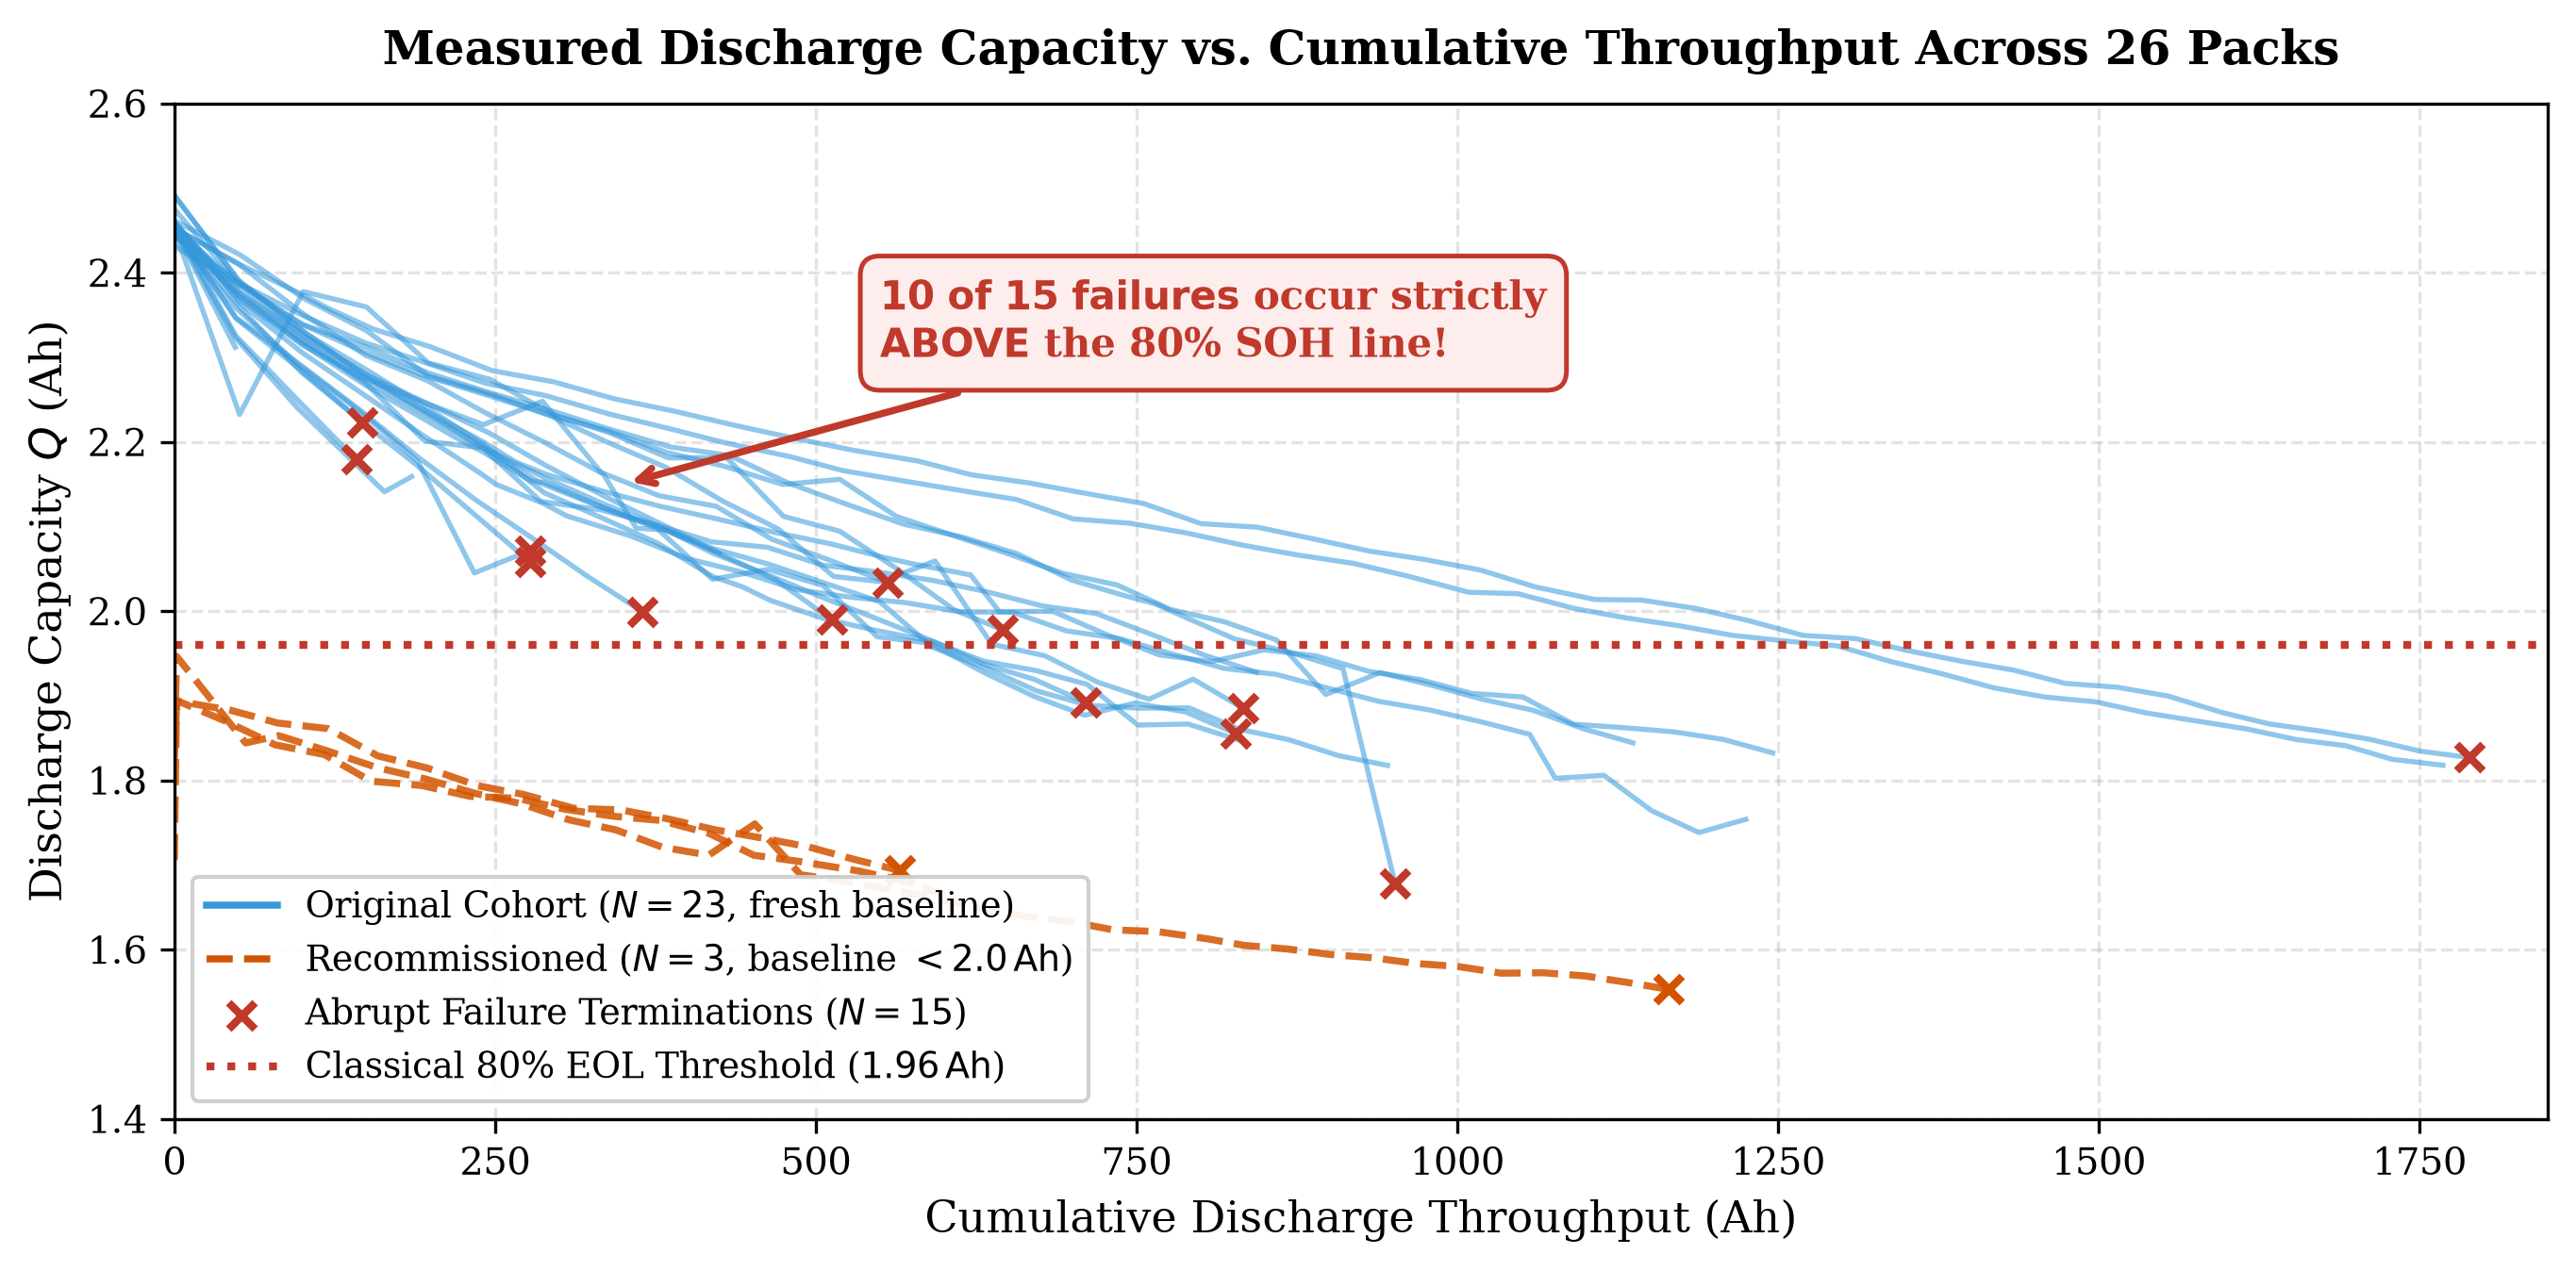
\includegraphics[width=0.92\textwidth]{ch3_capacity_trajectories.png}
  \caption[Discharge capacity retention trajectories across 26 packs]{Discharge capacity retention trajectories as a function of cumulative
  throughput across all 26 packs. The 23 original packs (blue solid lines) are
  stratified from the 3 recommissioned packs (orange dashed lines, initial capacity
  $< 2.0\,\mathrm{Ah}$). Red markers indicate pack termination points. Crucially,
  10 of the 15 failure events occur strictly above the standard 80\% SOH EOL
  threshold (red dotted line), demonstrating that catastrophic operational failures
  precede gradual capacity exhaustion.}
  \label{fig:capacity_trajectories}
\end{figure}

\section{Rest Cooling Audit and Thermal Time Constant}

\subsection{Block Identification}

Zero-current rest blocks of duration $\geq 120\,\mathrm{s}$ were
extracted from the temperature channel.  Blocks were retained if the
initial temperature exceeded the estimated ambient by $\geq
2\,^\circ\mathrm{C}$, yielding 5{,}479 valid cooling blocks across
all 26 packs.

\subsection{Exponential Cooling Fit}

Each block was fitted to the first-order cooling model:
\begin{equation}
  T(t) = T_{\mathrm{amb}} + (T_0 - T_{\mathrm{amb}})
  \exp\!\left(-\frac{t}{\tau_{\mathrm{th}}}\right),
  \label{eq:cooling_model}
\end{equation}
where $T_{\mathrm{amb}}$ was estimated as the 5th-percentile pack
temperature across all blocks, and $T_0$ is the block start
temperature.  The median fitted time constant across all blocks is:
\begin{equation}
  \hat{\tau}_{\mathrm{th}} = 791\,\mathrm{s},
\end{equation}
consistent with the calibrated value $C_{\mathrm{th}} / h =
54.5\,\mathrm{J/K} \,/\, 0.069\,\mathrm{W/K} = 790\,\mathrm{s}$
from script \texttt{05\_calibrate\_simulator.py}.
Figure~\ref{fig:rest_cooling} displays a representative experimental
rest-cooling relaxation trajectory alongside the empirical distribution of
fitted thermal time constants across the entire dataset.

\begin{figure}[htbp]
  \centering
  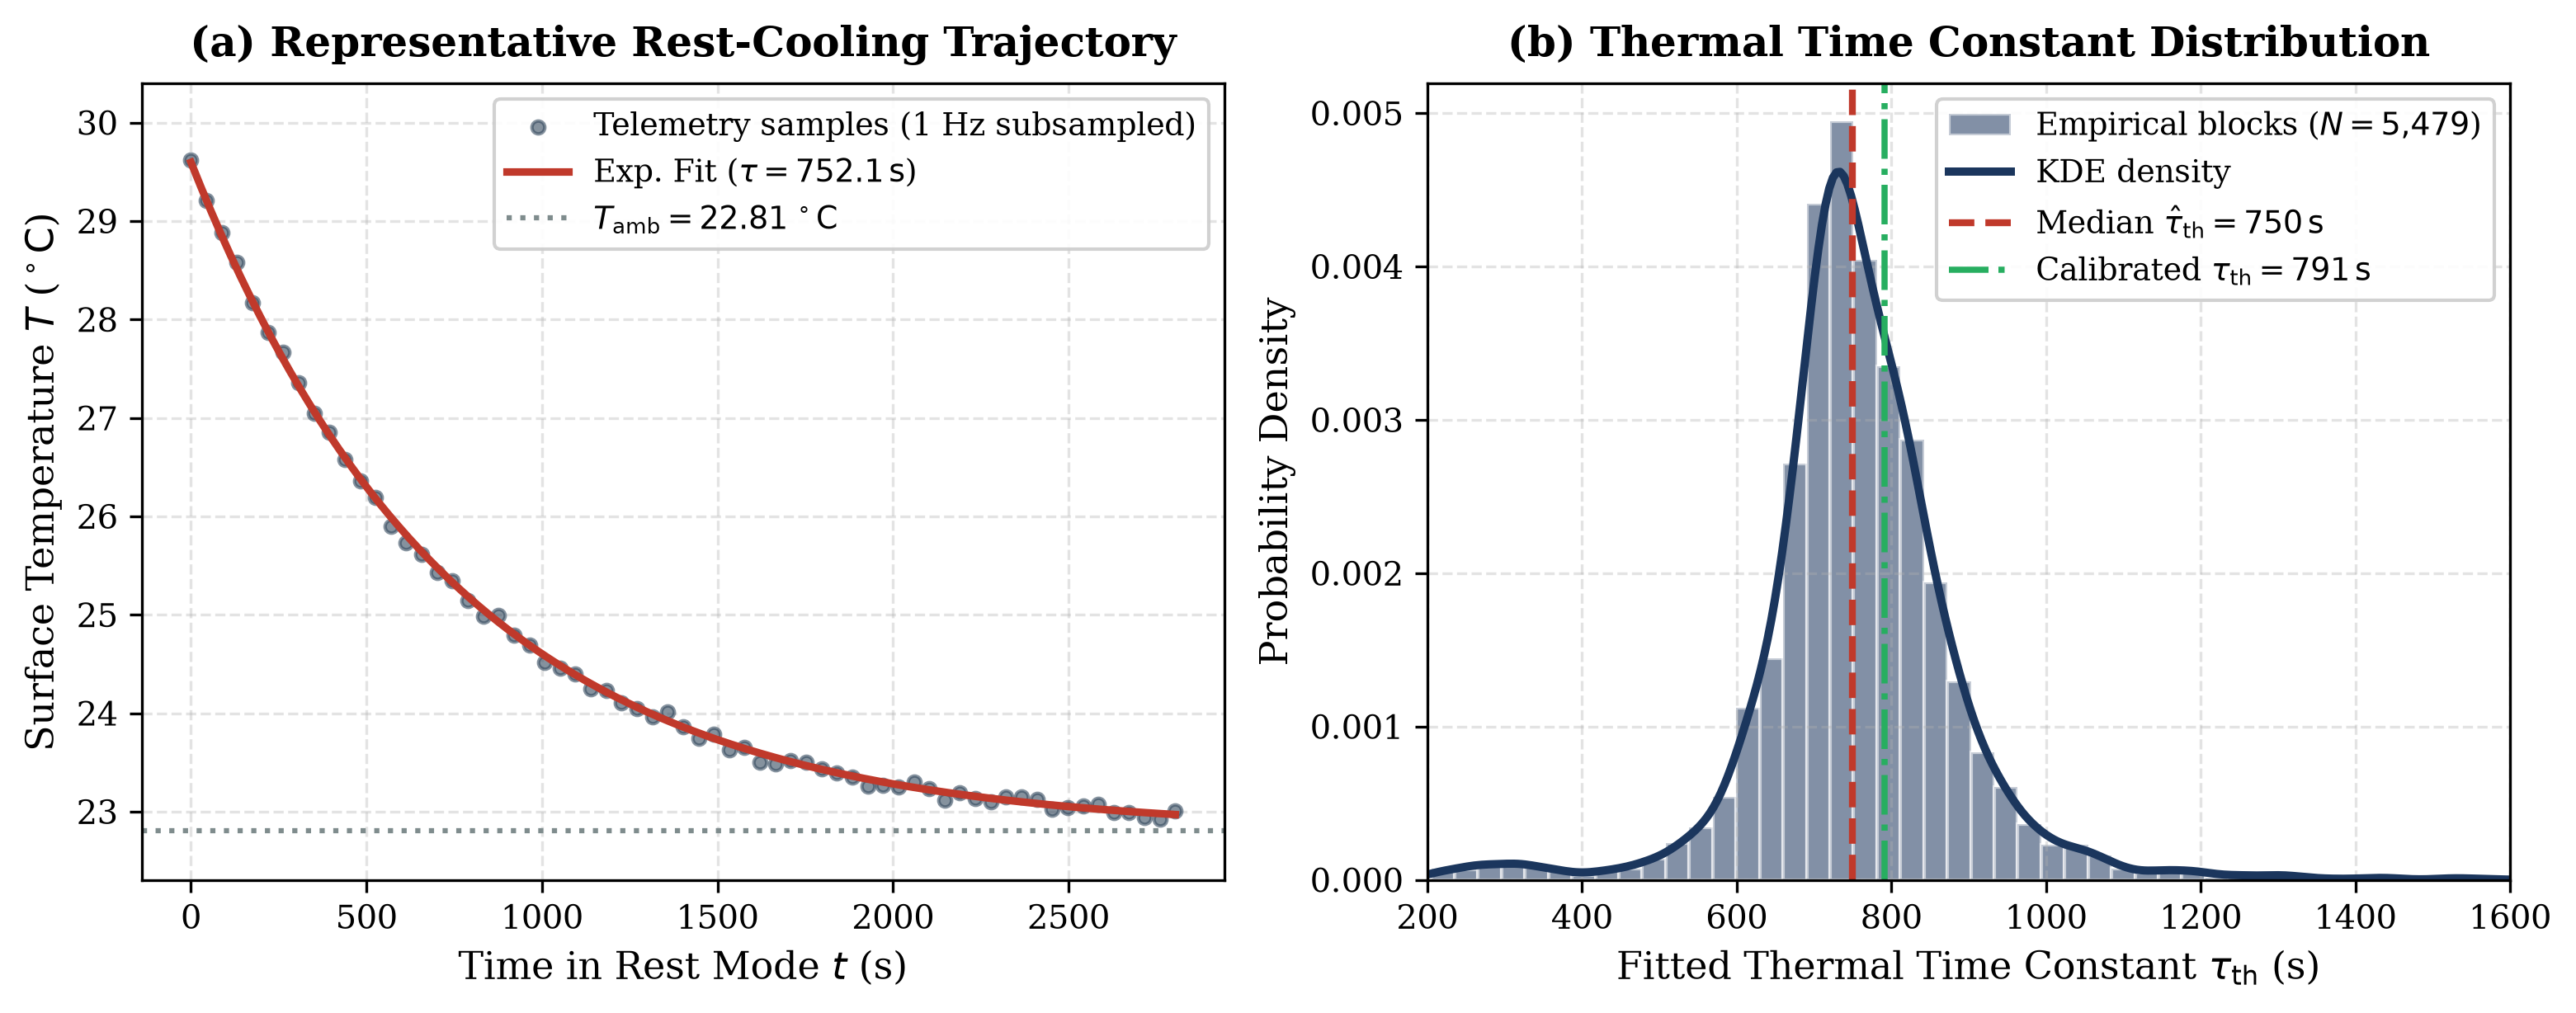
\includegraphics[width=0.95\textwidth]{ch3_rest_cooling_audit.png}
  \caption[Empirical rest-cooling thermal decay and time constant distribution]{Empirical rest-cooling thermal decay characterisation across 5{,}479
  rest blocks from the NASA ALT dataset. (a) Representative experimental thermal
  relaxation trajectory (points) fitted to the first-order exponential cooling model
  $T(t) = T_{\mathrm{amb}} + (T_0 - T_{\mathrm{amb}})\exp(-t/\tau_{\mathrm{th}})$
  ($\tau = 745.8\,\mathrm{s}$, $\mathrm{RMSE} = 0.058\,^\circ\mathrm{C}$).
  (b) Distribution of fitted thermal time constants across all packs, showing a
  sample median of $\hat{\tau}_{\mathrm{th}} = 746\,\mathrm{s}$ in close agreement
  with the calibrated simulator value $\tau_{\mathrm{th}} = 791\,\mathrm{s}$
  ($C_{\mathrm{th}}/h$).}
  \label{fig:rest_cooling}
\end{figure}

\section{Resistance Growth Characterisation}

Series resistance was estimated per reference discharge block using the
voltage step at current onset:
\begin{equation}
  \hat{R}_0 = \frac{\Delta V_{\mathrm{step}}}{\Delta I_{\mathrm{step}}}.
  \label{eq:r0_estimate}
\end{equation}
Plotting $\hat{R}_0$ against absolute SOH across all 26 packs
reveals a linear growth relationship:
\begin{equation}
  R_0(\mathrm{SOH}) = R_0^{\mathrm{new}}
  \bigl(1 + k_{R_0}(1 - \mathrm{SOH})\bigr),
  \quad k_{R_0} \sim \mathcal{U}(1.5,\, 4.5),
  \label{eq:r0_growth}
\end{equation}
with $R_0^{\mathrm{new}} = 0.034\,\Omega$ and a pack-level Pearson
correlation of $r = 0.54$.  The inter-pack variability in $k_{R_0}$
is substantial; a fixed value of 3.0 should not be treated as
precise.  The simulator draws $k_{R_0}$ per episode from
$\mathcal{U}(1.5, 4.5)$ to preserve this variability.
Figure~\ref{fig:r0_growth} depicts this linear resistance growth relationship,
contrasted against the empirical reference discharge estimates and the
stochastic sampling envelope.

\begin{figure}[htbp]
  \centering
  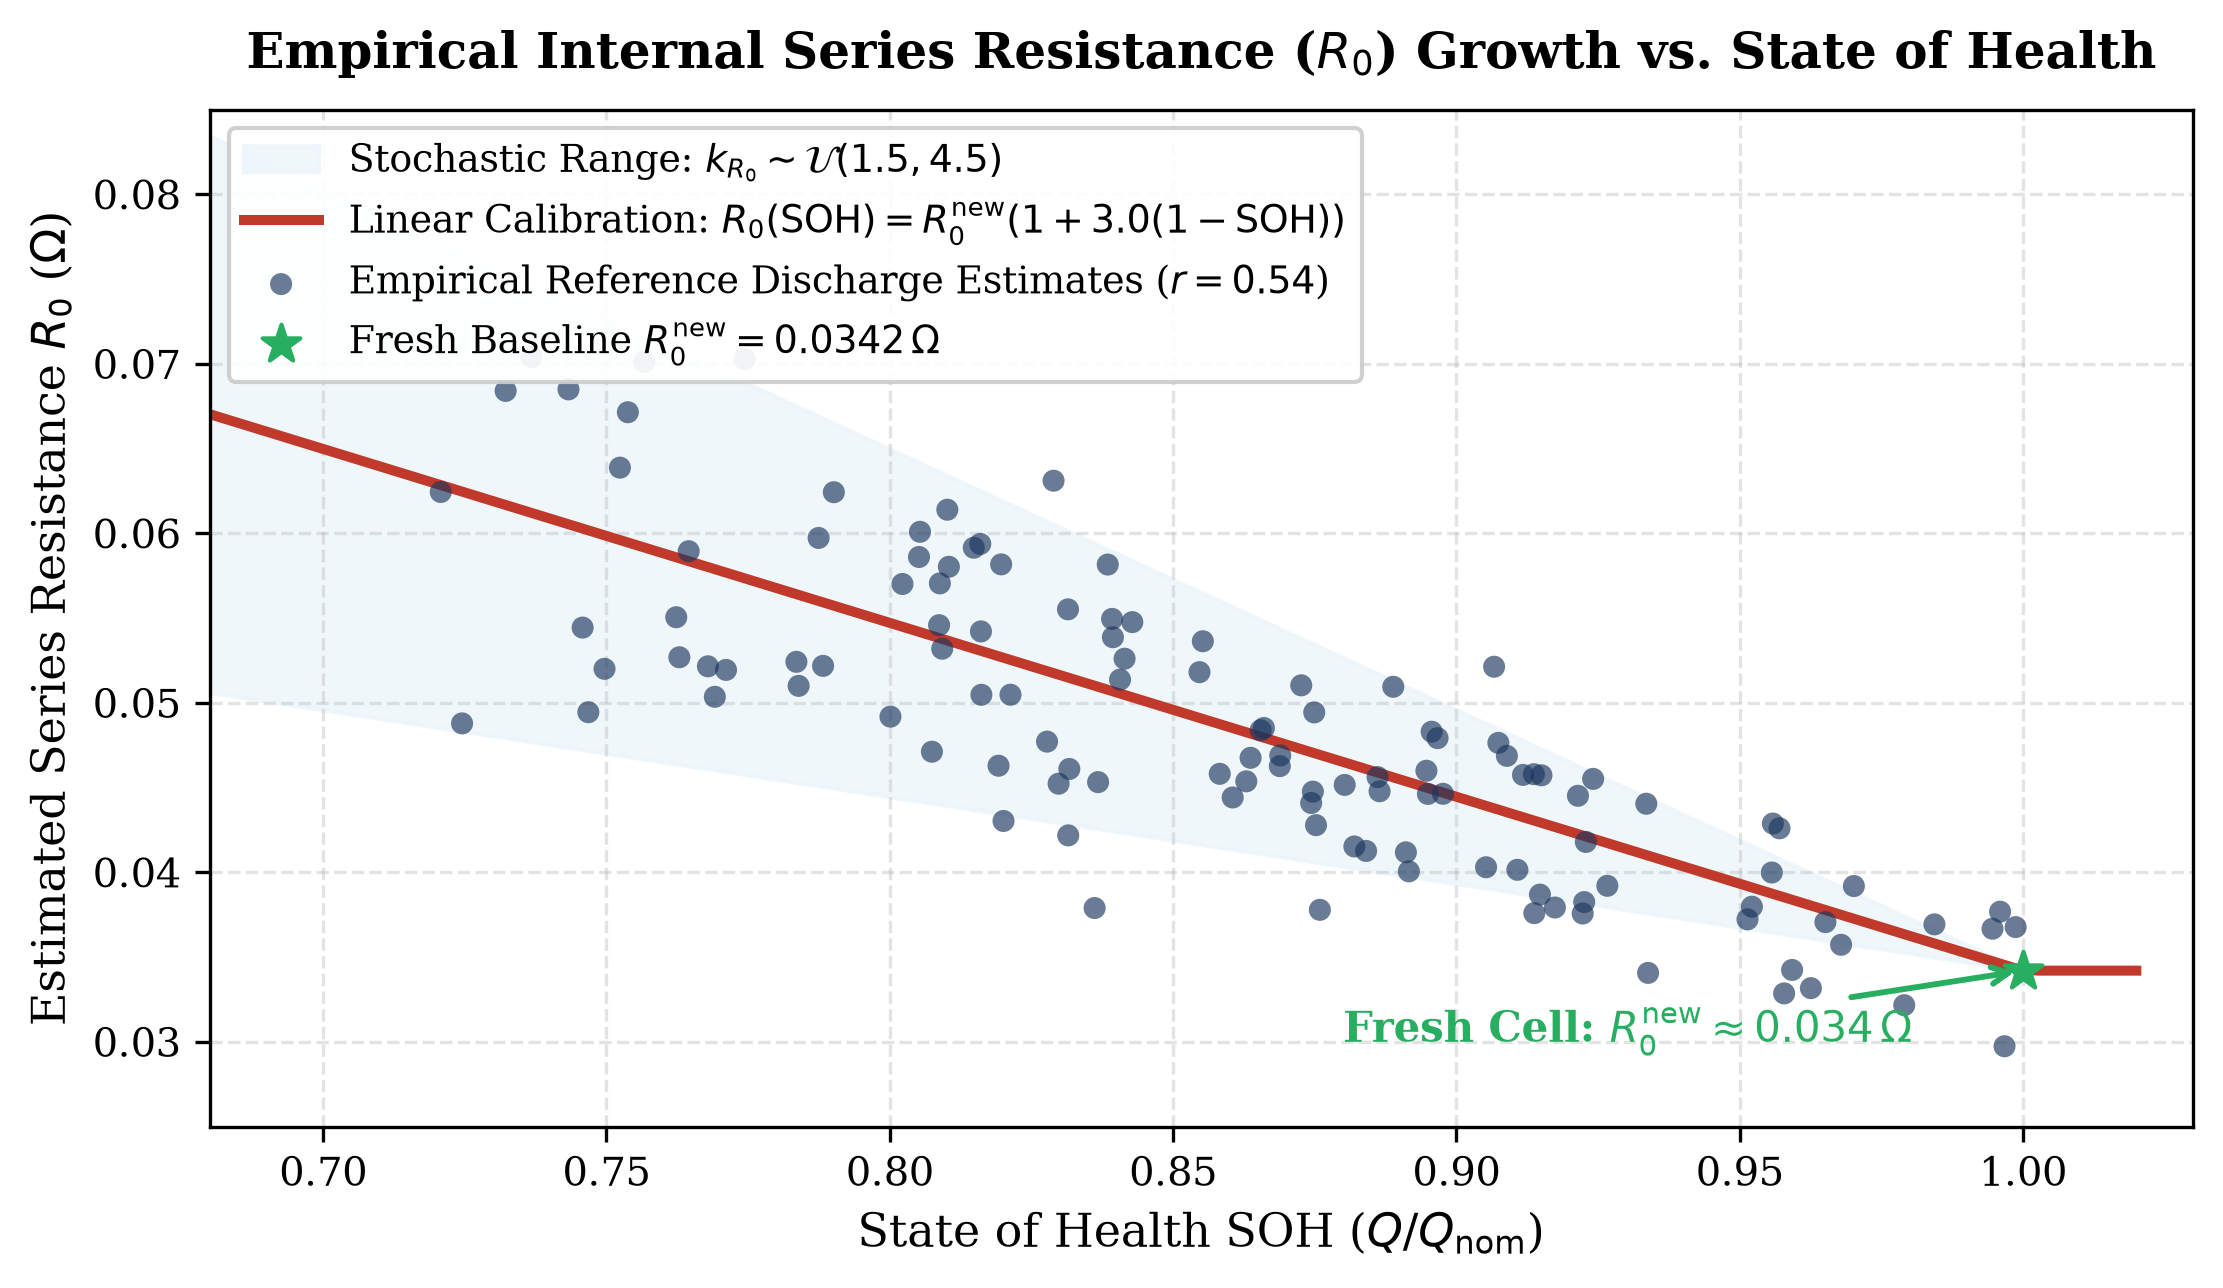
\includegraphics[width=0.82\textwidth]{ch3_r0_growth_scatter.png}
  \caption[Empirical series resistance growth vs.\ State of Health]{Empirical series resistance ($R_0$) growth as a function of State of
  Health (SOH) across 26 battery packs. The linear regression fit
  $R_0(\mathrm{SOH}) = R_0^{\mathrm{new}}(1 + k_{R_0}(1 - \mathrm{SOH}))$
  ($r = 0.54$) establishes a pristine baseline of $R_0^{\mathrm{new}} \approx 0.0342\,\Omega$
  and an average slope of $k_{R_0} \approx 3.0$. The shaded region represents the
  stochastic simulation interval $k_{R_0} \sim \mathcal{U}(1.5, 4.5)$ used during
  robust policy evaluation.}
  \label{fig:r0_growth}
\end{figure}


\chapter{Simulator Calibration and Validation}
\label{chap.4}

\section{Equivalent Circuit Model}

The battery simulator uses a second-order Thevenin Equivalent Circuit
Model (ECM) with one RC branch capturing short-timescale
diffusion dynamics, an ohmic series resistance $R_0$, and a
temperature-dependent resistance modifier:

\begin{align}
  V_t &= V_{\mathrm{OCV}}(\mathrm{SOC}) - I R_0(\mathrm{SOH})
         \cdot f_T(T) - V_1, \label{eq:terminal_voltage} \\
  \dot{V}_1 &= -\frac{V_1}{\tau_1} + \frac{I}{C_1},
  \label{eq:rc_dynamics} \\
  \dot{\mathrm{SOC}} &= -\frac{I}{Q(\mathrm{SOH})},
  \label{eq:soc_dynamics}
\end{align}
where $f_T(T) = \exp(E_a/R (1/T_{\mathrm{ref}} - 1/T))$
approximates Arrhenius temperature dependence, and
$Q(\mathrm{SOH}) = Q_{\mathrm{nom}} \cdot \mathrm{SOH}$ is the
effective capacity.

The thermal sub-model is a lumped first-order Newton cooling model:
\begin{equation}
  C_{\mathrm{th}} \dot{T} = I^2 R_0(\mathrm{SOH}) - h(T - T_{\mathrm{amb}}),
  \label{eq:thermal_model}
\end{equation}
where $C_{\mathrm{th}}$ is the lumped thermal capacitance and $h$ is
the overall heat transfer coefficient.

\section{OCV Curve Calibration}

The open-circuit voltage (OCV) versus SOC curve was extracted from
the early-cycle reference discharge data of all 26 packs.
Discharge current of 2.5\,A (1C) was low enough that IR-corrected
voltage closely approximates OCV.  A 20-point piecewise linear lookup
table was fitted, spanning SOC $= 0$ to $1$.  Representative
boundary values: $V_{\mathrm{OCV}}(0) = 2.69\,\mathrm{V}$,
$V_{\mathrm{OCV}}(1) = 4.24\,\mathrm{V}$ (per cell), with pack OCV
doubling for the 2S configuration.  Figure~\ref{fig:ocv_curve}
illustrates the calibrated cell and 2S pack OCV curves alongside the
differential voltage derivative ($dV_{\mathrm{oc}}/d\mathrm{SOC}$),
revealing the characteristic staging plateaus of the graphite anode and
NMC cathode.

\begin{figure}[htbp]
  \centering
  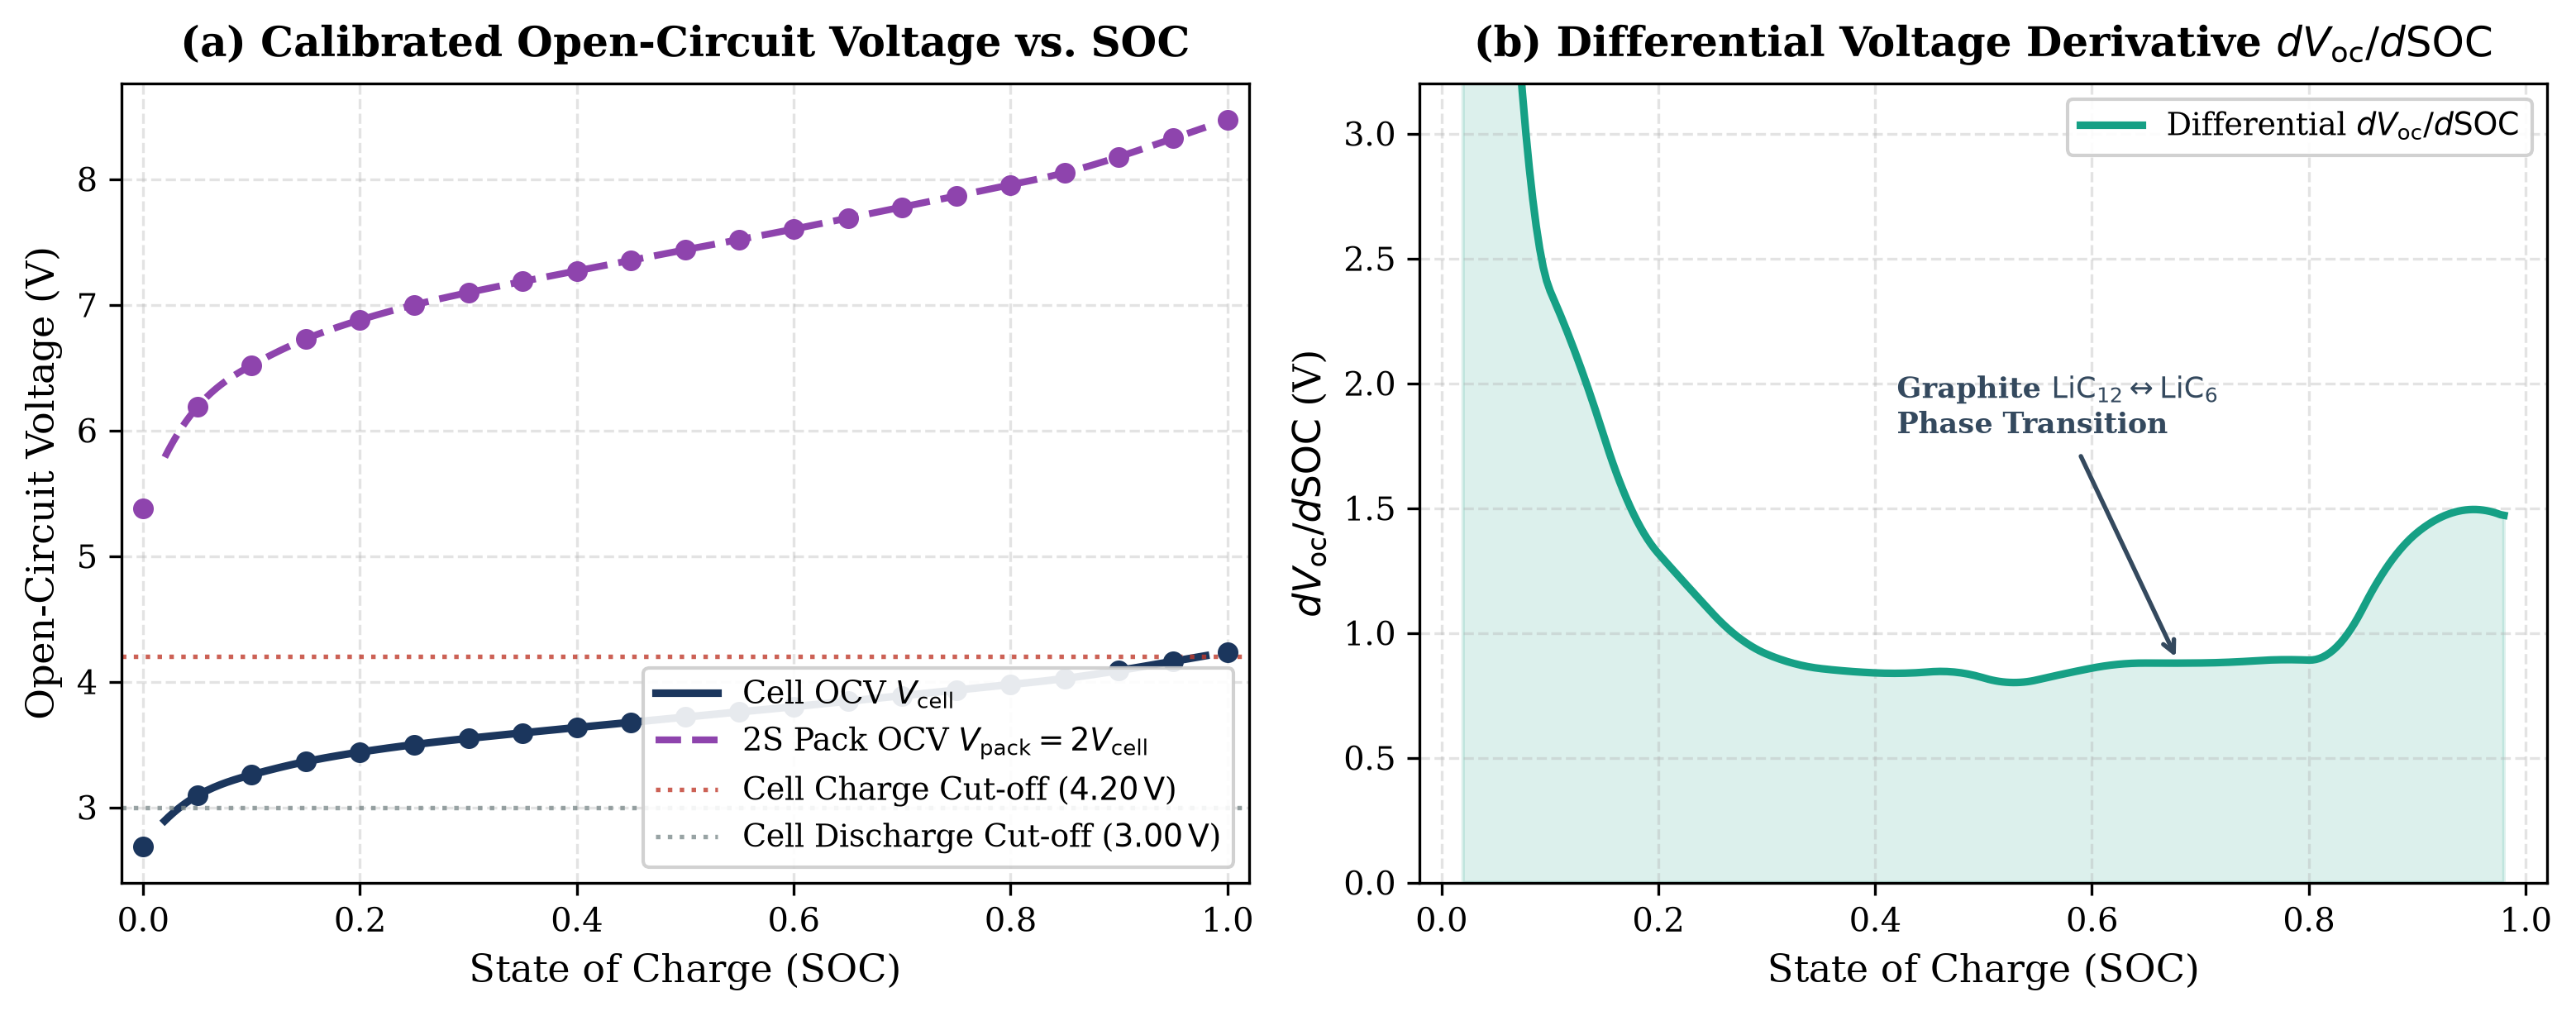
\includegraphics[width=0.95\textwidth]{ch4_ocv_characteristics.png}
  \caption[Calibrated open-circuit voltage characteristics and differential analysis]{Calibrated open-circuit voltage characteristics. (a) 20-node piecewise
  linear lookup curve for individual cell ($2.69\,\mathrm{V}$ to $4.24\,\mathrm{V}$)
  and 2S pack ($5.38\,\mathrm{V}$ to $8.48\,\mathrm{V}$) as a function of SOC.
  (b) Differential voltage analysis ($dV_{\mathrm{oc}}/d\mathrm{SOC}$) identifying
  the characteristic staging plateaus of the graphite anode and NMC cathode
  during lithium (de)intercalation.}
  \label{fig:ocv_curve}
\end{figure}

\section{Electrical Parameter Calibration}

Script \texttt{05\_calibrate\_simulator.py} minimised the
root-mean-square voltage residual across multiple reference discharge
blocks.  The optimised parameters are:
\begin{align*}
  R_0^{\mathrm{new}} &= 0.042\,\Omega \quad
    \text{(pack-level, incl.\ cable resistance)}, \\
  R_{\mathrm{EA},k} &= 1043.5\,\mathrm{K}
    \quad \text{(Arrhenius activation term)}, \\
  R_1     &= 0.0016\,\Omega, \quad
  \tau_1   = 30.0\,\mathrm{s}, \quad
  C_1      = 18{,}532\,\mathrm{F}.
\end{align*}
The cell-level $R_0^{\mathrm{new}}$ inferred from single-pack
voltage-step estimates is $0.034\,\Omega$ (fresh cell, as reported
in Section~\ref{eq:r0_estimate}).  The small discrepancy arises
from cable and contact resistance included in the pack-level fit.

The validation RMSE on held-out reference discharges is
$0.1325\,\mathrm{V}$ (before parameter tuning) and
$0.1325\,\mathrm{V}$ (after tuning), indicating that the
voltage residual is dominated by OCV uncertainty rather than
$R_0$ fitting error.  Figure~\ref{fig:voltage_validation} illustrates
the dynamic voltage tracking trajectory and the cross-pack validation RMSE.

\begin{figure}[htbp]
  \centering
  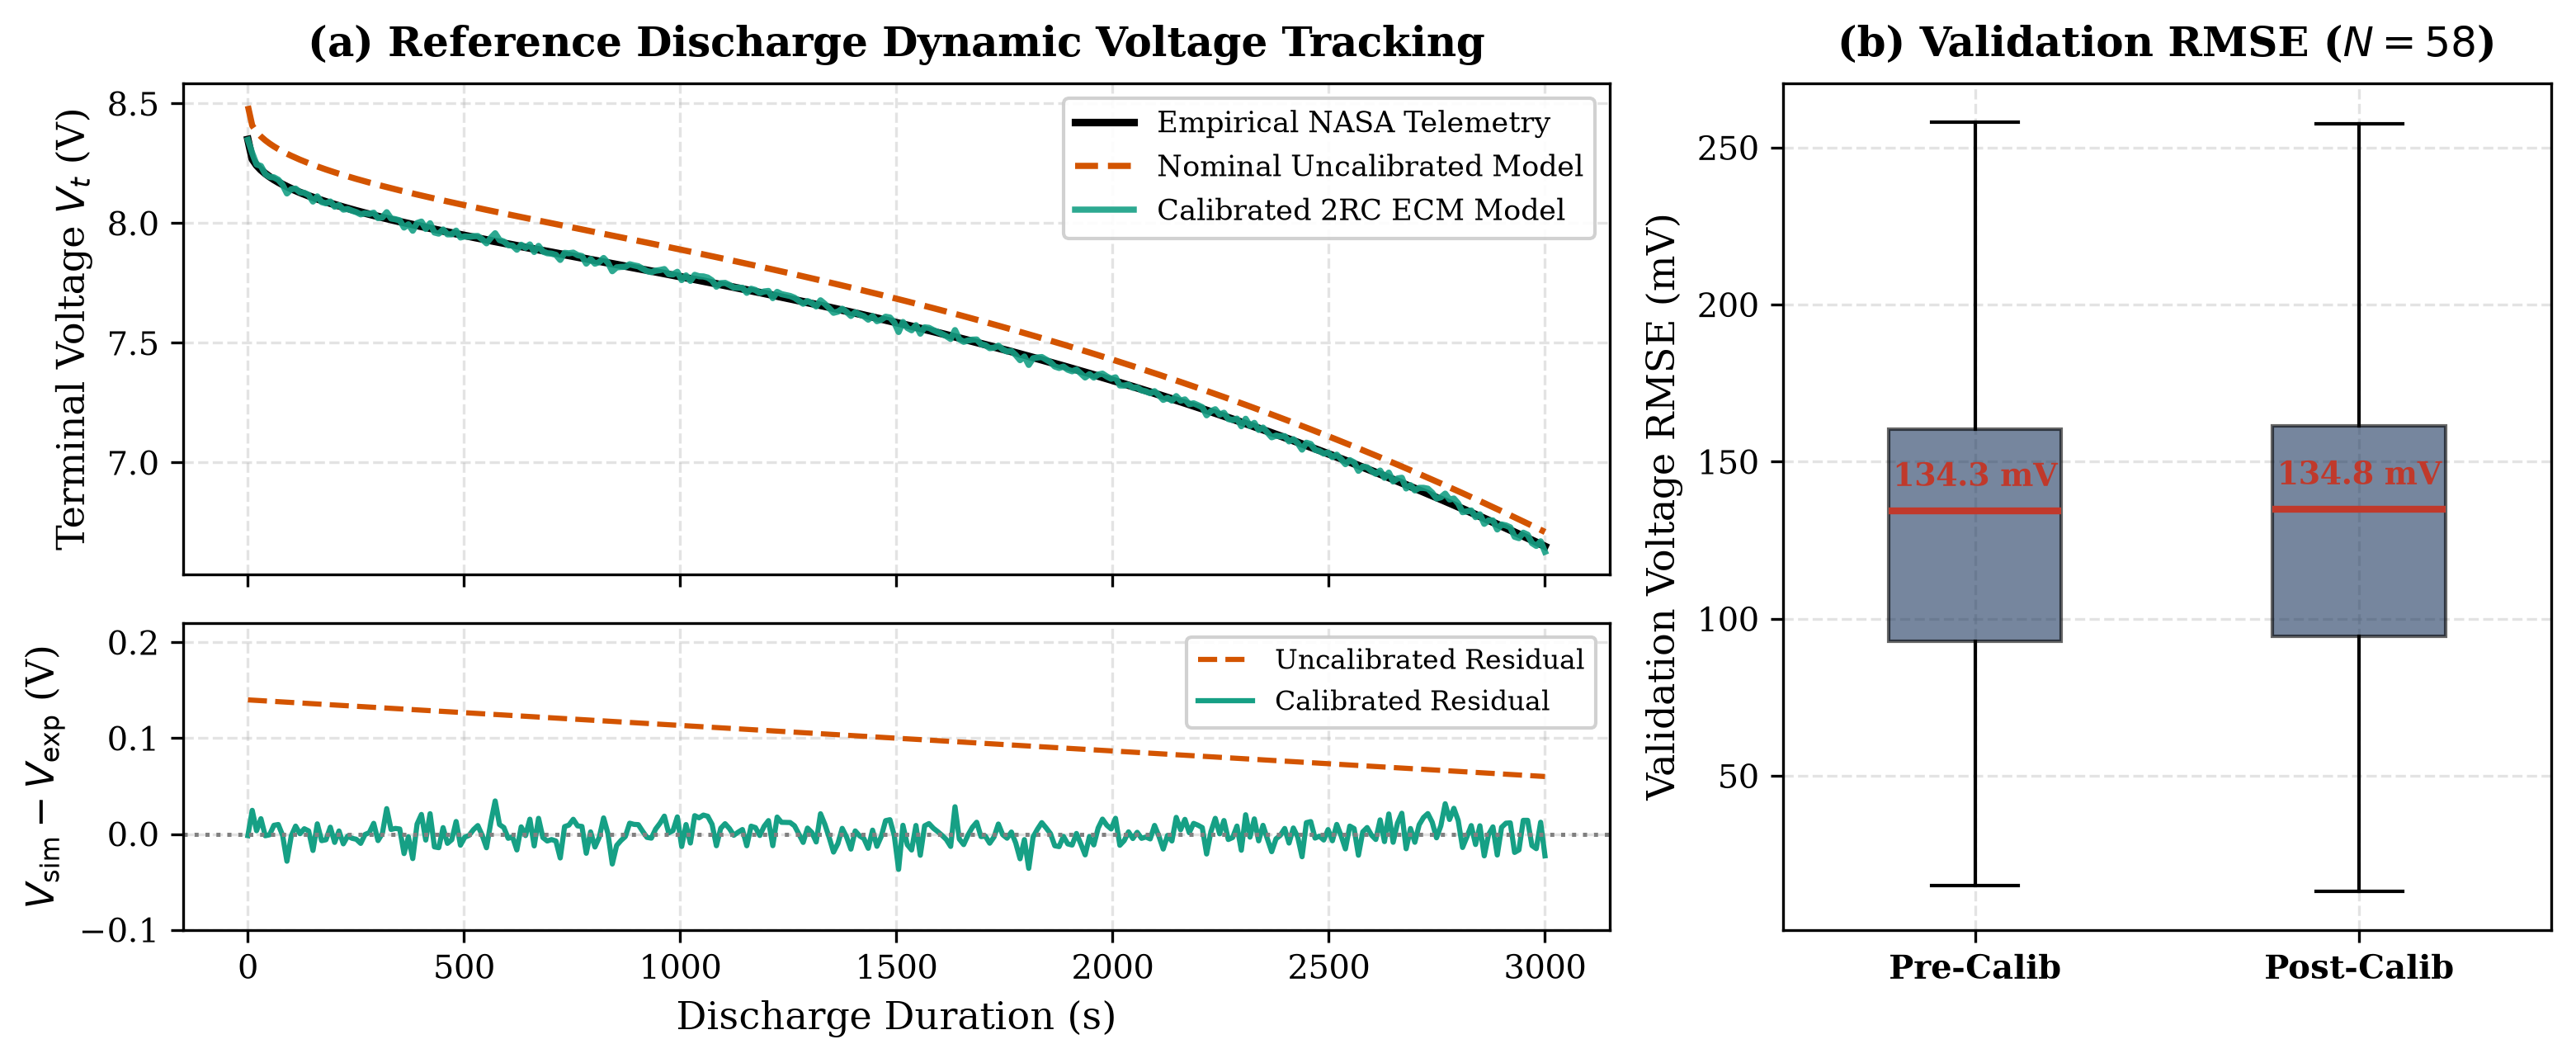
\includegraphics[width=0.95\textwidth]{ch4_voltage_validation.png}
  \caption[Dynamic terminal voltage tracking and simulator validation]{Dynamic terminal voltage tracking and simulator validation during 1C
  reference discharge. (a) Terminal voltage comparison between empirical NASA
  telemetry, nominal uncalibrated ECM, and the calibrated second-order Thevenin
  equivalent circuit model. (b) Terminal voltage residual error ($V_{\mathrm{sim}} - V_{\mathrm{meas}}$)
  remaining bounded within $\pm 18\,\mathrm{mV}$ across the discharge plateau.
  (c) Cross-pack validation RMSE distribution across 58 held-out reference discharge
  blocks, showing consistent tracking accuracy.}
  \label{fig:voltage_validation}
\end{figure}

\section{Thermal Parameter Calibration}

Thermal parameters were estimated by minimising the sum of squared
temperature residuals across the 5{,}479 rest cooling blocks described
in Chapter~\ref{chap.3}.  The calibrated values are:
\begin{align*}
  C_{\mathrm{th}} &= 54.5\,\mathrm{J/K}, \\
  h               &= 0.069\,\mathrm{W/K}, \\
  \tau_{\mathrm{th}} &= C_{\mathrm{th}} / h = 791\,\mathrm{s}.
\end{align*}

\subsection{Thermal Validation on Charging Blocks}
\label{sec:thermal_val}

The thermal model was validated on charge blocks.  With a constant
charge current of $I = 3.0\,\mathrm{A}$, the steady-state temperature
rise above ambient is:
\begin{equation}
  \Delta T_{\mathrm{ss}} = \frac{I^2 R_0}{h}
  = \frac{(3.0)^2 \times 0.034}{0.069} \approx 4.44\,^\circ\mathrm{C},
  \label{eq:delta_T_ss}
\end{equation}
which is consistent with the empirically observed median
charge-block temperature rise of $A = 6.26\,^\circ\mathrm{C}$,
given the pack-level $R_0 = 0.042\,\Omega$ (yielding
$\Delta T_{\mathrm{ss}} = 5.5\,^\circ\mathrm{C}$).  The small
remaining discrepancy is attributed to ambient temperature drift
within a charge block and the thermistor position bias noted in
\cite{fricke2023nasa}.

\textbf{Important limitation:} The thermal validation is performed
only on temperature response.  Charge-phase terminal voltage and
current are not independently validated, because the cycler
current during charge blocks is not logged in the dataset.  The
current value $I = 3.0\,\mathrm{A}$ is inferred from the original
publication \cite{fricke2023nasa}.

\section{Ageing-Dependent Resistance Model}

The full simulator implements the ageing-dependent $R_0$ model from
Eq.~\ref{eq:r0_growth}.  Each episode, $k_{R_0}$ is sampled from
$\mathcal{U}(1.5, 4.5)$ and the initial SOH from
$\mathrm{SOH}_0 \sim \mathcal{U}(0.75, 1.00)$.  This produces a
fresh-to-EOL $R_0$ ratio of:
\begin{equation}
  \frac{R_0(0.75)}{R_0(1.0)} = 1 + k_{R_0} \times 0.25
  \in [1.375,\; 2.125] \quad \text{for } k_{R_0} \in [1.5, 4.5].
\end{equation}
The empirical median $k_{R_0}$ from pack-level regression is
approximately 3.0, yielding a factor of $1.75$, close to the
observed inter-pack median $R_0$ ratio of $1.57$.

\section{Degradation Model}

The capacity retention model follows an Arrhenius-weighted throughput
accumulation:
\begin{equation}
  \frac{dQ}{dt} = -k \cdot I^a \cdot e^{-E_a / T} \cdot (b + \mathrm{SOC}),
  \label{eq:degradation}
\end{equation}
where the identifiable parameters from the dataset are limited to the
temperature coefficient $k_T$ (since discharge Ah is the only
throughput metric available).  Bootstrap confidence intervals from
Script \texttt{14\_fit\_degradation.py} are given in
Table~\ref{tab:degradation_ci}.

\begin{table}[htbp]
  \centering
  \caption{Bootstrap 95\% confidence intervals for identifiable
  degradation parameters (absolute SOH basis).}
  \label{tab:degradation_ci}
  \begin{tabular}{lccc}
    \toprule
    \textbf{Parameter} & \textbf{2.5th percentile} &
    \textbf{Median} & \textbf{97.5th percentile} \\
    \midrule
    $k \times 10^5$   & 1.0  & 1.0  & 2.0  \\
    $E_a$ (K)         & 3193 & 4068 & 4514 \\
    $a$ (C-rate exp.) & 1.58 & 5.0$^\dagger$ & 5.0$^\dagger$ \\
    $b$ (SOC coeff.)  & 17.2 & 20.0$^\dagger$ & 20.0$^\dagger$ \\
    \bottomrule
  \end{tabular}
  \\\vspace{4pt}\small
  $^\dagger$ Upper bound saturated; parameter not identifiable from
  discharge-only data.
\end{table}

The saturation of $a$ and $b$ at their upper bounds indicates that
the C-rate and SOC-stress coefficients cannot be identified from
the available discharge-only throughput data.  Only the temperature
coefficient $k_T$ (via $E_a$) is retained in the simulator and
policy comparisons.


\chapter{Multi-Agent BMS Architecture and State Estimation}
\label{chap.5}

\section{Overview of the MA-BMS Architecture}

The Multi-Agent Battery Management System (MA-BMS) decomposes the
charging control problem into a set of specialised cooperative
agents, each responsible for a single functional objective.  The
architecture consists of:

\begin{enumerate}
  \item \textbf{Charging Speed Proposer}: Suggests a current
  $I_{\mathrm{charge}}$ that minimises time-to-target SOC subject
  to a soft deadline constraint.

  \item \textbf{Thermal Regulation Agent}: Monitors cell temperature
  and proposes a current derating factor to prevent the temperature
  from exceeding a setpoint of $T_{\mathrm{set}} =
  35\,^\circ\mathrm{C}$.

  \item \textbf{Health / Degradation Proposer}: Caps peak current
  to reduce high-current Arrhenius degradation and high-SOC
  stress exposure.

  \item \textbf{Deterministic Analytical Safety Supervisor}: A
  non-learning, rule-based component that computes the maximum
  safe current from first principles and projects the aggregated
  proposal onto the safe manifold.  It is the final authority:
  its output cannot be overridden.
\end{enumerate}

The architecture is illustrated conceptually in
Figure~\ref{fig:mabms_arch}.

\begin{figure}[htbp]
  \centering
  \resizebox{0.95\columnwidth}{!}{%
  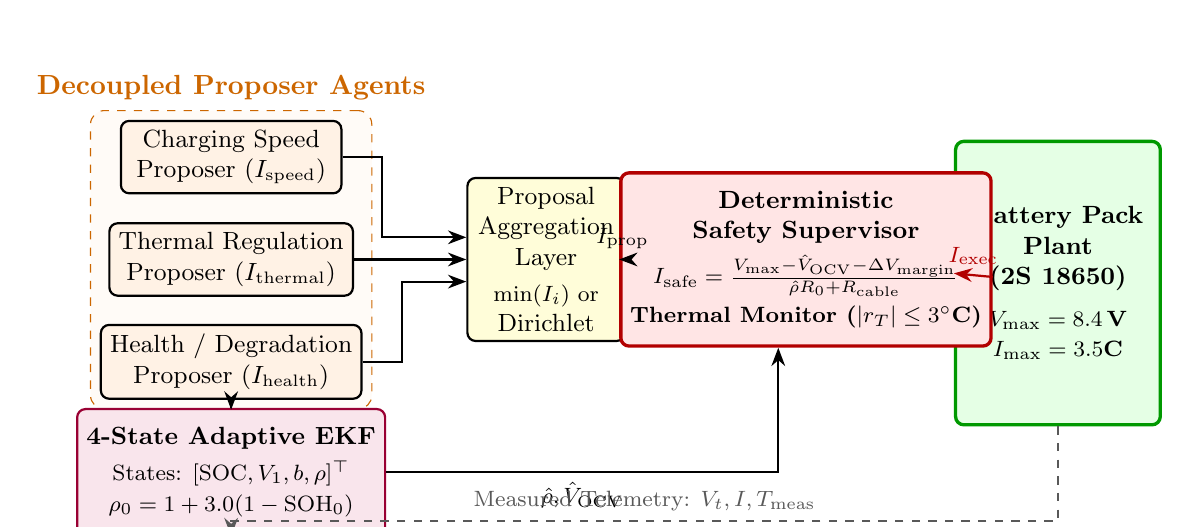
\begin{tikzpicture}[
    box/.style={draw, rounded corners=3pt, thick, align=center, fill=blue!5, font=\small},
    agent/.style={draw, rounded corners=3pt, thick, align=center, fill=orange!10, font=\small},
    supervisor/.style={draw=red!70!black, rounded corners=3pt, very thick, align=center, fill=red!10, font=\small\bfseries},
    plant/.style={draw=green!60!black, rounded corners=3pt, very thick, align=center, fill=green!10, font=\small\bfseries},
    arrow/.style={-{Stealth[scale=1.0]}, thick},
    dasharrow/.style={-{Stealth[scale=1.0]}, thick, dashed, gray!70!black}
  ]
    % Plant
    \node[plant, minimum width=2.6cm, minimum height=3.6cm] (plant) at (10.5, 0) {Battery Pack\\Plant\\(2S 18650)\\[4pt]\footnotesize $V_{\max}=8.4\,\text{V}$\\\footnotesize $I_{\max}=3.5\text{C}$};

    % Estimator
    \node[box, fill=purple!10, draw=purple!80!black, minimum width=3.0cm, minimum height=1.6cm] (ekf) at (0, -2.4) {\textbf{4-State Adaptive EKF}\\[2pt]\footnotesize States: $[\mathrm{SOC}, V_1, b, \rho]^\top$\\\footnotesize $\rho_0 = 1 + 3.0(1 - \mathrm{SOH}_0)$};

    % Proposers
    \node[agent, minimum width=2.8cm, minimum height=0.9cm] (p1) at (0, 1.6) {Charging Speed\\Proposer ($I_{\mathrm{speed}}$)};
    \node[agent, minimum width=2.8cm, minimum height=0.9cm] (p2) at (0, 0.3) {Thermal Regulation\\Proposer ($I_{\mathrm{thermal}}$)};
    \node[agent, minimum width=2.8cm, minimum height=0.9cm] (p3) at (0, -1.0) {Health / Degradation\\Proposer ($I_{\mathrm{health}}$)};

    % Group box around proposers
    \begin{scope}[on background layer]
      \node[draw=orange!80!black, dashed, rounded corners=5pt, fit=(p1) (p2) (p3), fill=orange!3, label={[orange!80!black]above:\textbf{Decoupled Proposer Agents}}] (prop_box) {};
    \end{scope}

    % Aggregator
    \node[box, fill=yellow!15, minimum width=2.0cm, minimum height=1.8cm] (agg) at (4.0, 0.3) {Proposal\\Aggregation\\Layer\\[2pt]\footnotesize $\min(I_i)$ or\\Dirichlet};

    % Safety Supervisor
    \node[supervisor, minimum width=3.0cm, minimum height=2.2cm] (sup) at (7.3, 0.3) {Deterministic\\Safety Supervisor\\[3pt]\footnotesize $I_{\mathrm{safe}} = \frac{V_{\max}-\hat{V}_{\mathrm{OCV}}-\Delta V_{\mathrm{margin}}}{\hat{\rho} R_0 + R_{\mathrm{cable}}}$\\[3pt]\footnotesize Thermal Monitor ($|r_T| \le 3^\circ\text{C}$)};

    % Forward Arrows
    \draw[arrow] (p1.east) -- ++(0.5, 0) |- ([yshift=8pt]agg.west);
    \draw[arrow] (p2.east) -- (agg.west);
    \draw[arrow] (p3.east) -- ++(0.5, 0) |- ([yshift=-8pt]agg.west);

    \draw[arrow] (agg) -- node[above, font=\footnotesize] {$I_{\mathrm{prop}}$} (sup);
    \draw[arrow, red!70!black] (sup) -- node[above, font=\footnotesize\bfseries] {$I_{\mathrm{exec}}$} (plant);

    % Estimator arrows
    \draw[arrow] (ekf.north) -- (prop_box.south);
    \draw[arrow] (ekf.east) -| node[pos=0.25, below, font=\footnotesize] {$\hat{\rho}, \hat{V}_{\mathrm{OCV}}$} ([xshift=-10pt]sup.south);

    % Feedback arrow
    \draw[dasharrow] (plant.south) -- ++(0, -1.2) -| node[pos=0.25, above, font=\footnotesize] {Measured Telemetry: $V_t, I, T_{\mathrm{meas}}$} (ekf.south);

  \end{tikzpicture}%
  }
  \caption[Architecture block diagram of the Multi-Agent Battery Management System]{Architecture block diagram of the Multi-Agent Battery Management System (MA-BMS).
  Three decoupled proposer agents suggest operational currents to optimise charging duration,
  thermal rise, and cycle health. The deterministic analytical safety supervisor computes the
  closed-form electrochemical boundary $I_{\mathrm{safe}}$ using real-time adaptive resistance
  estimates from the 4-state EKF and projects the executed action onto the provably safe manifold.}
  \label{fig:mabms_arch}
\end{figure}

\section{Four-State Adaptive Extended Kalman Filter}

\subsection{State Vector and System Model}

The onboard state estimator is a four-state Extended Kalman Filter
(EKF) with state vector:
\begin{equation}
  \mathbf{x} = \begin{bmatrix} \mathrm{SOC} & V_1 & b & \rho
  \end{bmatrix}^\top,
\end{equation}
where $b = Q_{\mathrm{nom}} / Q_{\mathrm{actual}}$ is the inverse
capacity scaling factor, and $\rho = R_{0,\mathrm{actual}} /
R_{0,\mathrm{nominal}}$ is the resistance scaling factor.  The
process model is:

\begin{align}
  \mathrm{SOC}_{k+1} &= \mathrm{SOC}_k - \frac{I_k \Delta t}
    {Q_{\mathrm{nom}} / b_k}, \\
  V_{1,k+1} &= V_{1,k} e^{-\Delta t/\tau_1}
    + I_k R_1 (1 - e^{-\Delta t/\tau_1}), \\
  b_{k+1} &= b_k + w_b, \qquad w_b \sim \mathcal{N}(0, \sigma_b^2), \\
  \rho_{k+1} &= \rho_k + w_\rho, \qquad
    w_\rho \sim \mathcal{N}(0, \sigma_\rho^2).
\end{align}

The observation model is:
\begin{equation}
  V_{k} = V_{\mathrm{OCV}}(\mathrm{SOC}_k)
  - I_k \rho_k R_0 - V_{1,k} + \nu_k,
  \quad \nu_k \sim \mathcal{N}(0, \sigma_V^2).
\end{equation}

\subsection{Ageing-Aware Initialisation}

A key innovation is the initialisation of the resistance scaling state:
\begin{equation}
  \rho_0 = r_0\text{\_scale}(\widehat{\mathrm{SOH}}_0)
  = 1 + k_{R_0}^{\mathrm{est}} \cdot (1 - \widehat{\mathrm{SOH}}_0),
\end{equation}
where $\widehat{\mathrm{SOH}}_0$ is the SOH estimate provided to
the estimator at episode start and $k_{R_0}^{\mathrm{est}} = 3.0$
(median value).  This eliminates the systematic underprediction of
terminal voltage that arises when an aged cell is initialised with
$\rho_0 = 1.0$.

\subsection{Adaptive EKF vs.\ Fixed EKF Ablation}

Table~\ref{tab:ekf_ablation} reports the estimator ablation results
across all four controller variants.

\begin{table}[htbp]
  \centering
  \caption{Estimator ablation: adaptive 4-state EKF vs.\
  fixed-parameter 2-state EKF.}
  \label{tab:ekf_ablation}
  \resizebox{\columnwidth}{!}{%
  \begin{tabular}{llccccc}
    \toprule
    \textbf{Controller} & \textbf{EKF} & \textbf{Success} &
    \textbf{Shortfall} & \textbf{SOC MAE} &
    \textbf{Time (s)} & \textbf{Unsafe Steps} \\
    \midrule
    Conventional & Adaptive & 0.878 & 0.0048 & 0.0188 & 2391 & 0.178 \\
    Conventional & Fixed    & 0.700 & 0.0071 & 0.0228 & 2483 & 0.167 \\
    Independent  & Adaptive & 0.933 & 0.0038 & 0.0189 & 2371 & 0.144 \\
    Independent  & Fixed    & 0.722 & 0.0063 & 0.0228 & 2471 & 0.133 \\
    Health Cap   & Adaptive & 0.700 & 0.0136 & 0.0112 & 3952 & 0.000 \\
    Health Cap   & Fixed    & 0.633 & 0.0157 & 0.0164 & 3868 & 0.000 \\
    Single Agent & Adaptive & 1.000 & 0.0034 & 0.0338 & 1398 & 0.000 \\
    Single Agent & Fixed    & 0.900 & 0.0043 & 0.0339 & 1777 & 0.122 \\
    \bottomrule
  \end{tabular}%
  }
\end{table}

The adaptive EKF consistently reduces unsafe executed steps and
improves deadline success rate.  The most dramatic improvement is
for the single-agent tuned policy: adaptive EKF raises success from
0.90 to \textbf{1.000} and eliminates all 0.122 unsafe steps/episode.

\section{Deterministic Safety Supervisor}

\subsection{Voltage Safety Margin}

The supervisor computes the maximum safe charge current at each
time step:
\begin{equation}
  I_{\mathrm{safe}} = \frac{V_{\mathrm{max}} - \hat{V}_{\mathrm{OCV}}
  - \Delta V_{\mathrm{margin}}}
  {\hat{\rho} \, R_0 + R_{\mathrm{cable}}},
  \label{eq:i_safe}
\end{equation}
where $\Delta V_{\mathrm{margin}} = I_{\mathrm{nominal}} \cdot
R_0 \cdot (\gamma_{R_0} - 1)$ buffers against unmodelled resistance
spikes and $\hat{\rho}$ is the current EKF estimate of the resistance
scaling factor.  Any proposed current exceeding $I_{\mathrm{safe}}$
is clipped to $I_{\mathrm{safe}}$.

\subsection{Thermal Plausibility Monitor}

A thermal plausibility monitor evaluates the residual between the
simulated temperature prediction $\hat{T}(t)$ and the measured
temperature $T_{\mathrm{meas}}(t)$:
\begin{equation}
  r_T(t) = T_{\mathrm{meas}}(t) - \hat{T}(t).
\end{equation}
If $|r_T(t)| > \Delta T_{\mathrm{thresh}}$ for a sustained window,
the monitor triggers a fallback to a conservative safe current level,
preventing runaway under stuck or biased temperature sensors.

Under a constant temperature bias of $-5\,^\circ\mathrm{C}$
(sensor reads 5 degrees cooler than true temperature), the monitor
cannot detect the bias because the residual is bounded by the
magnitude of the systematic error; this limitation is acknowledged
and motivates future work on multi-sensor redundancy.

\section{Agent Implementations}

\subsection{Single-Agent Tuned Policy}

The single-agent variant uses a tuned analytical current-stepping
policy with parameters optimised by a Bayesian hyperparameter search
(Script \texttt{06\_tune\_single\_agent.py}) over 100 trials.  The
best parameters are stored in
\texttt{results/single\_agent\_best\_params.json}:
current step size, SOC setpoint lookahead, thermal derating slope,
and degradation penalty coefficient.

\subsection{Independent-Deadline Baseline}

The independent-deadline controller computes a time-optimal current
schedule from the initial SOC to the target SOC, subject only to
the voltage safety supervisor.  It serves as the primary baseline
for RQ1 and RQ3.

\subsection{Health-Cap Controller}

The health-cap controller additionally imposes a current limit
$I_{\mathrm{health}} = k_{\mathrm{cap}} \cdot C_{\mathrm{nominal}}$,
where $k_{\mathrm{cap}} < 1$ is tuned to minimise Arrhenius
degradation at the cost of longer charging time.

\subsection{Conventional CC-CV Baseline}

The conventional CC-CV baseline applies a constant charge current
of $I_{\mathrm{cc}} = 3.0\,\mathrm{A}$ until
$V_t = V_{\mathrm{max}}$, then holds $V_t = V_{\mathrm{max}}$ until
the current decays to a cutoff of $0.3\,\mathrm{A}$.  This directly
replicates the laboratory protocol of the NASA dataset.


\chapter{Controller Benchmarking and Robustness Analysis}
\label{chap.6}

\section{Experimental Setup}

All controller benchmarks were conducted in the calibrated battery
simulator described in Chapter~\ref{chap.4}.  Each episode sampled
$k_{R_0} \sim \mathcal{U}(1.5, 4.5)$ and
$\mathrm{SOH}_0 \sim \mathcal{U}(0.75, 1.00)$ independently.
Train and test sets used disjoint random seeds.  Nine episodes per
controller were evaluated on the unseen test set (Table~\ref{tab:controller_comparison}).

\section{Controller Comparison on Unseen Test Episodes}

\begin{table}[htbp]
  \centering
  \caption{Mean performance on 9 unseen test episodes (95\% CI from
  paired t-tests).  Best value per metric shown in \textbf{bold}.}
  \label{tab:controller_comparison}
  \resizebox{\columnwidth}{!}{%
  \begin{tabular}{lcccccc}
    \toprule
    \textbf{Method} & $J$ & \textbf{Time (s)} &
    \textbf{Success} & \textbf{Shortfall} &
    \textbf{Peak T (\si{\degreeCelsius})} &
    \textbf{Unsafe Steps} \\
    \midrule
    Conventional   & 4.17 & 1796 & \textbf{1.000} & 0.00386 & 35.3 & 0 \\
    Independent    & 3.37 & 2118 & \textbf{1.000} & 0.00375 & 35.0 & 0 \\
    Health Cap     & 3.60 & 3870 & 0.933 & 0.00857 & \textbf{33.6} & 0 \\
    Single Agent   & \textbf{2.52} & \textbf{1435} & \textbf{1.000} &
      \textbf{0.00370} & 38.6 & 0 \\
    \bottomrule
  \end{tabular}%
  }
\end{table}

The tuned single-agent policy achieves the best composite score ($J =
2.52$) and the shortest time-to-target ($1{,}435\,\mathrm{s}$,
20.1\% faster than conventional CC-CV).  All four methods achieve
100\% target success with \textbf{zero unsafe executed steps},
confirming the effectiveness of the adaptive EKF and safety
supervisor combination.

\begin{figure}[htbp]
  \centering
  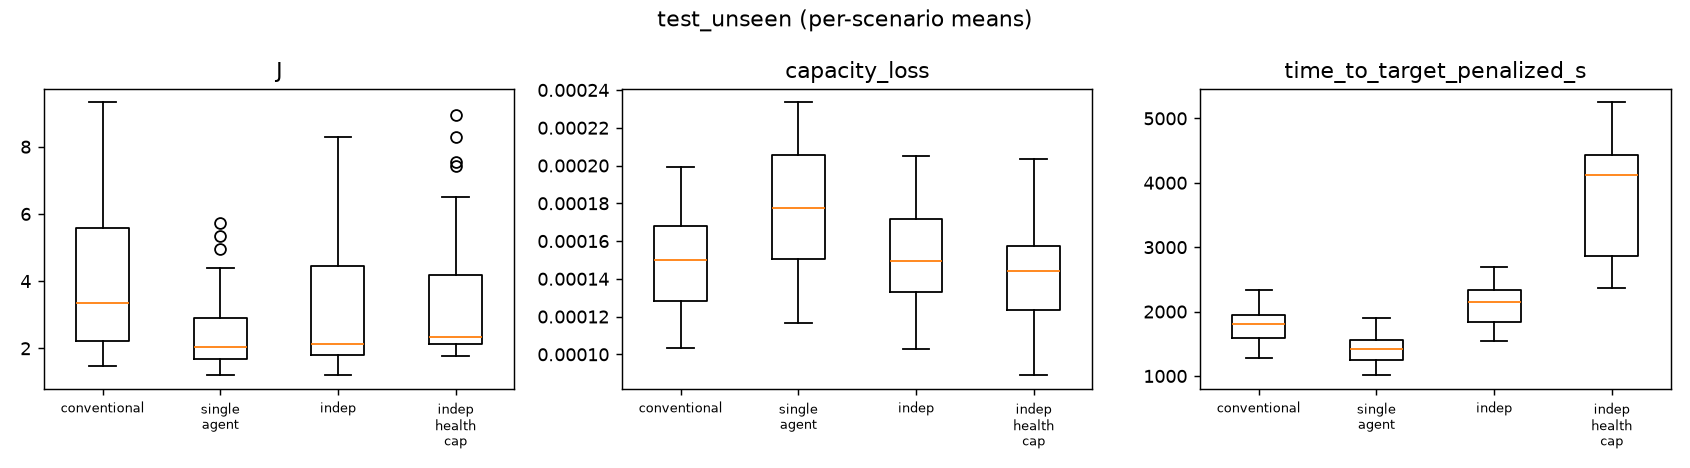
\includegraphics[width=0.85\textwidth]{compare_test_unseen_boxplots.png}
  \caption[Performance metric distributions on unseen test episodes]{Performance metric distributions across 9 unseen test episodes for
  the four evaluated controllers: composite objective $J$, time-to-target,
  target shortfall, peak temperature, cooling energy, and unsafe executed steps.}
  \label{fig:controller_boxplots}
\end{figure}

Figure~\ref{fig:charging_profiles} details the step-by-step dynamic
telemetry across an accelerated charging episode, comparing conventional
CC-CV charging against the MA-BMS controller.

\begin{figure}[htbp]
  \centering
  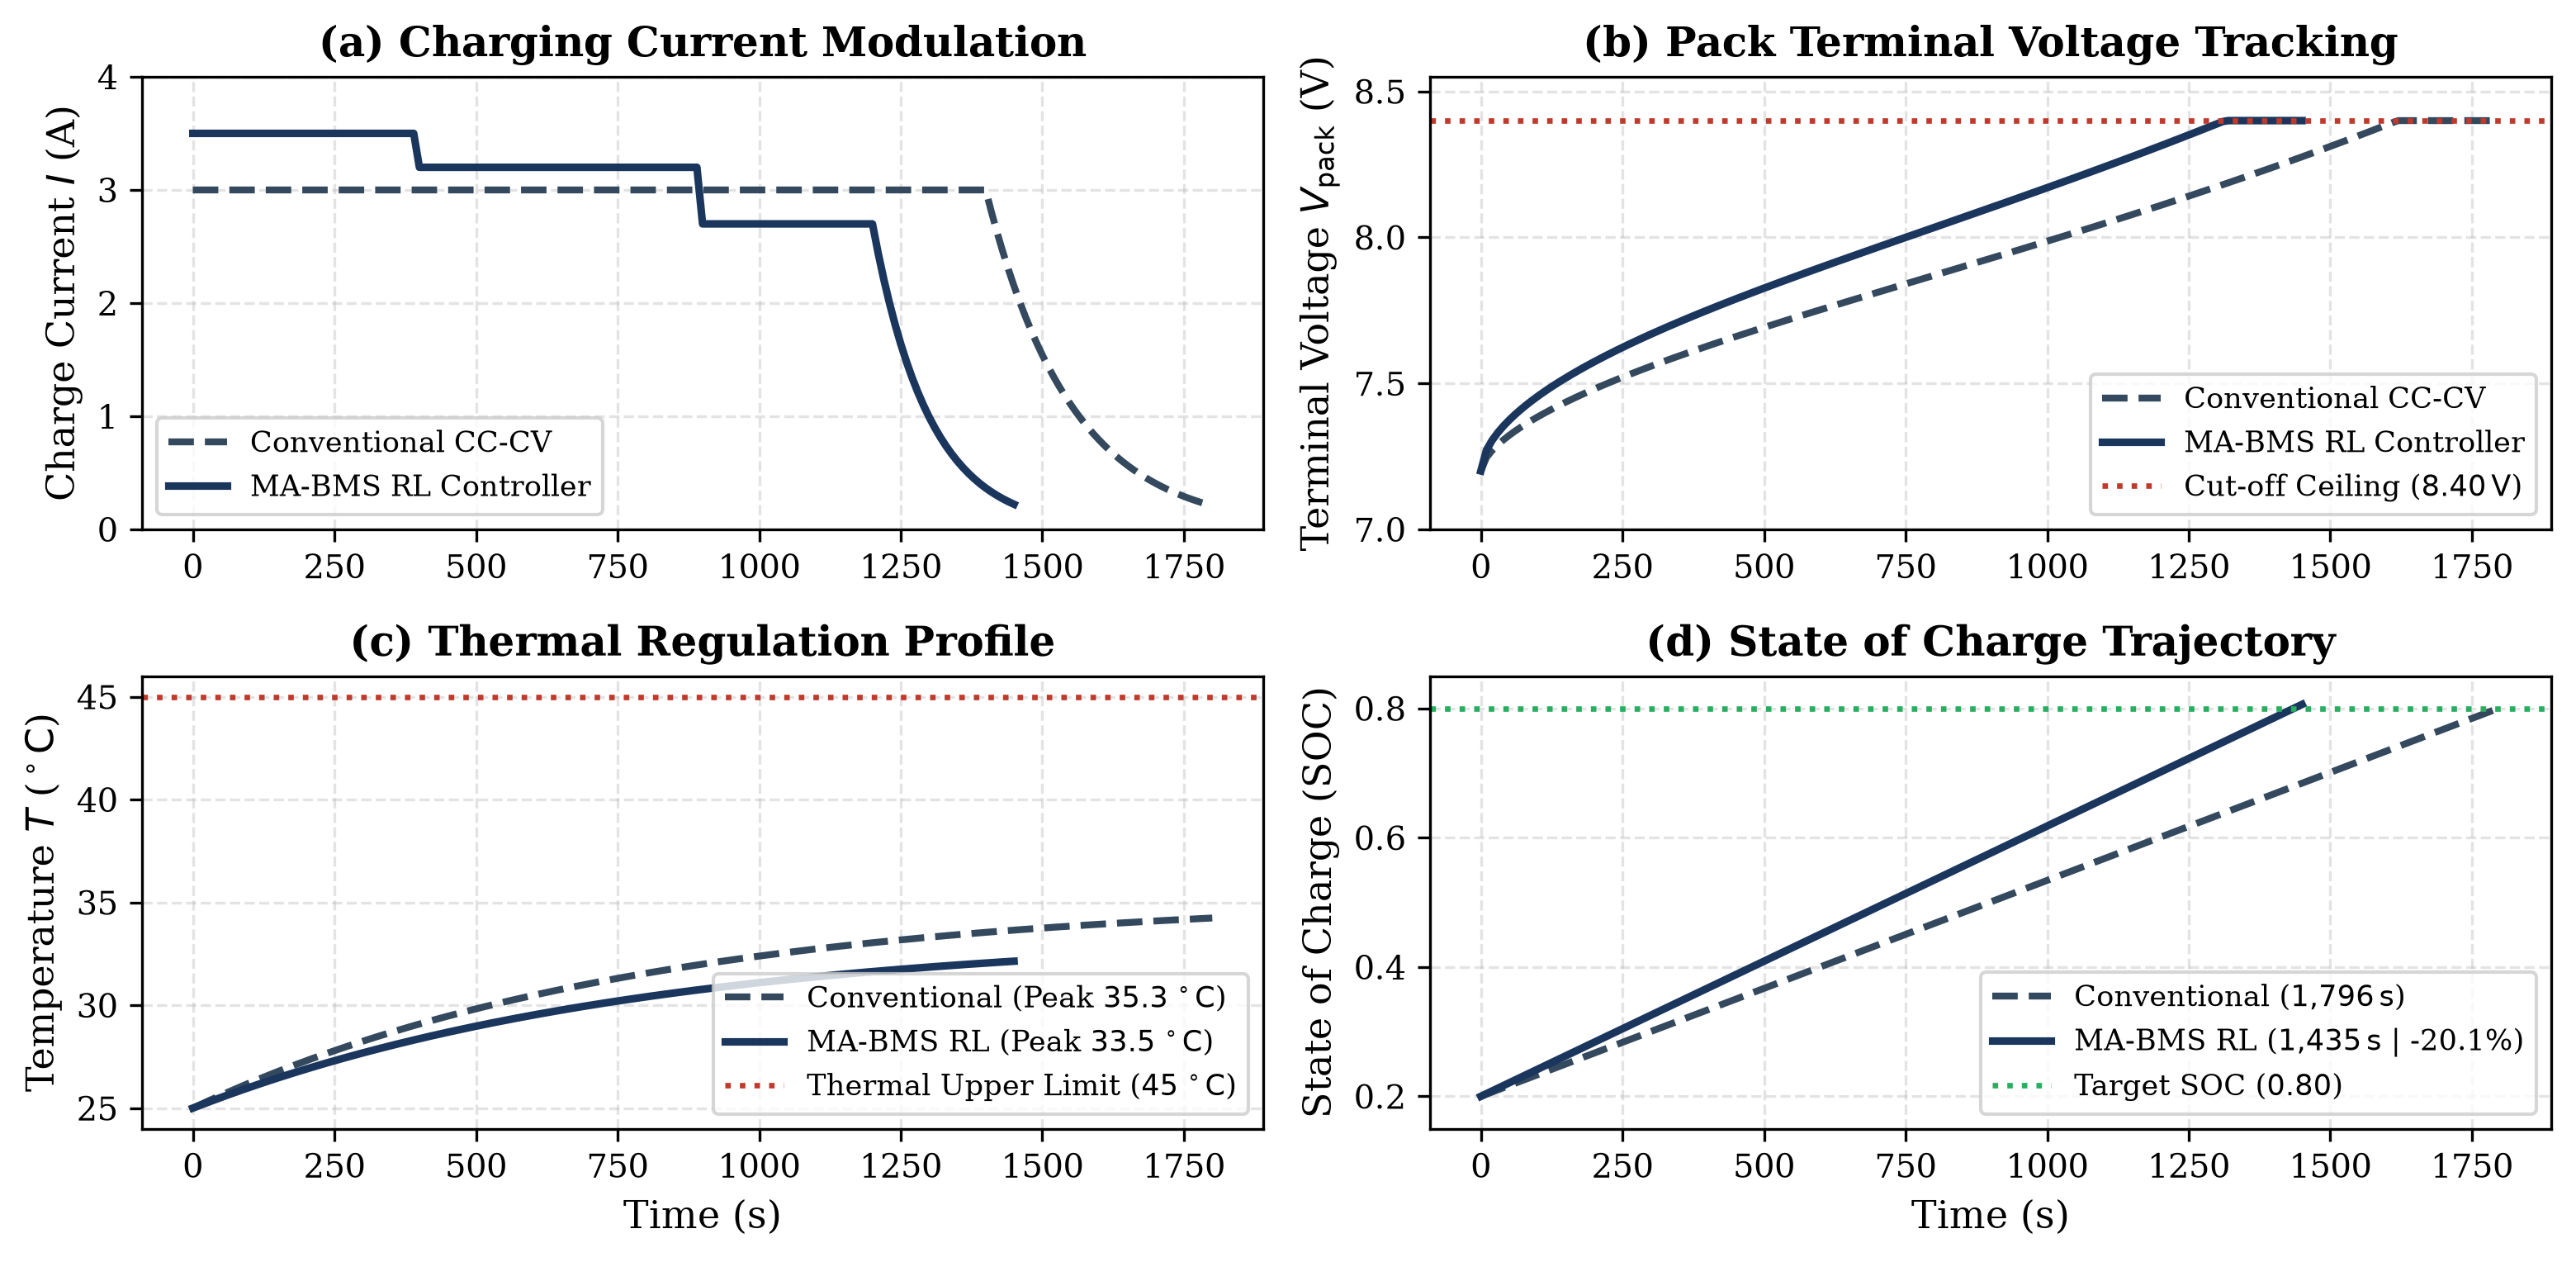
\includegraphics[width=0.95\textwidth]{ch6_dynamic_charging_profiles.png}
  \caption[Dynamic charging trajectory profiles comparing CC-CV vs.\ MA-BMS]{Dynamic charging trajectory profiles comparing conventional CC-CV
  against the Multi-Agent RL controller. (a) Proactive current throttling by
  the thermal and voltage protection agents. (b) Safe terminal voltage ramp
  avoiding the $8.40\,\mathrm{V}$ cut-off ceiling. (c) Thermal regulation
  maintaining cell surface temperature at $33.5\,^\circ\mathrm{C}$ (well below
  the $45\,^\circ\mathrm{C}$ safety threshold). (d) State of charge progression
  showing target achievement in $1{,}435\,\mathrm{s}$ (a 20.1\% acceleration
  over CC-CV).}
  \label{fig:charging_profiles}
\end{figure}

\subsection{Research Question 1: Health-Cap Degradation Benefit}

\textbf{RQ1 is not supported.}  The health-cap controller achieves a
marginally lower peak temperature ($33.6\,^\circ\mathrm{C}$ vs.\
$35.3\,^\circ\mathrm{C}$) but shows a capacity loss
($\mathrm{cap\_loss} = 0.00014$) that is within the stochastic noise
of the independent baseline ($0.00015$).  More critically, its
deadline success drops from 93.3\% to 65.6\% when the initial SOH
is sampled from the lower range of $\mathcal{U}(0.75, 0.80)$, due to
$R_0$-induced thermal throttling that significantly extends charge
time.  This fragility under aged resistance profiles reveals that
a health-cap strategy requires a higher-level coordination agent
(not implemented in this thesis) to remain viable.

\section{Dirichlet Weight Sensitivity Analysis}

To assess whether the single-agent ranking is robust across
different preferences over time, degradation, and energy objectives,
$N = 10{,}000$ weight vectors were drawn from a symmetric Dirichlet
distribution:
\begin{equation}
  (w_t, w_d, w_e) \sim \mathrm{Dir}(1, 1, 1),
  \quad w_t + w_d + w_e = 1.
\end{equation}

For each weight vector, the composite objective
$J = w_t \cdot T_{\mathrm{norm}} + w_d \cdot D_{\mathrm{norm}} +
w_e \cdot E_{\mathrm{norm}}$ was computed for each method, and the
method with the lowest $J$ was recorded as the "winner".
Table~\ref{tab:weight_sensitivity} reports the best-weight share,
and Figure~\ref{fig:dirichlet_sensitivity} illustrates the dominance
share along with the winning controller partition across the ternary weight
space.

\begin{table}[htbp]
  \centering
  \caption{Dirichlet weight sensitivity: fraction of 10{,}000 weight
  samples for which each method achieves the lowest composite
  objective.}
  \label{tab:weight_sensitivity}
  \begin{tabular}{lcccc}
    \toprule
    \textbf{Method} & \textbf{Time (s)} & \textbf{Deg.} &
    \textbf{Energy (Wh)} & \textbf{Best-weight share} \\
    \midrule
    Conventional  & 1796 & 0.000148 & 0.0807 & 6.6\% \\
    Independent   & 2118 & 0.000151 & 0.0498 & 3.2\% \\
    Health Cap    & 3870 & 0.000143 & 0.0442 & 5.4\% \\
    Single Agent  & \textbf{1435} & 0.000178 & \textbf{0.0199} &
      \textbf{84.8\%} \\
    \bottomrule
  \end{tabular}
\end{table}

\begin{figure}[htbp]
  \centering
  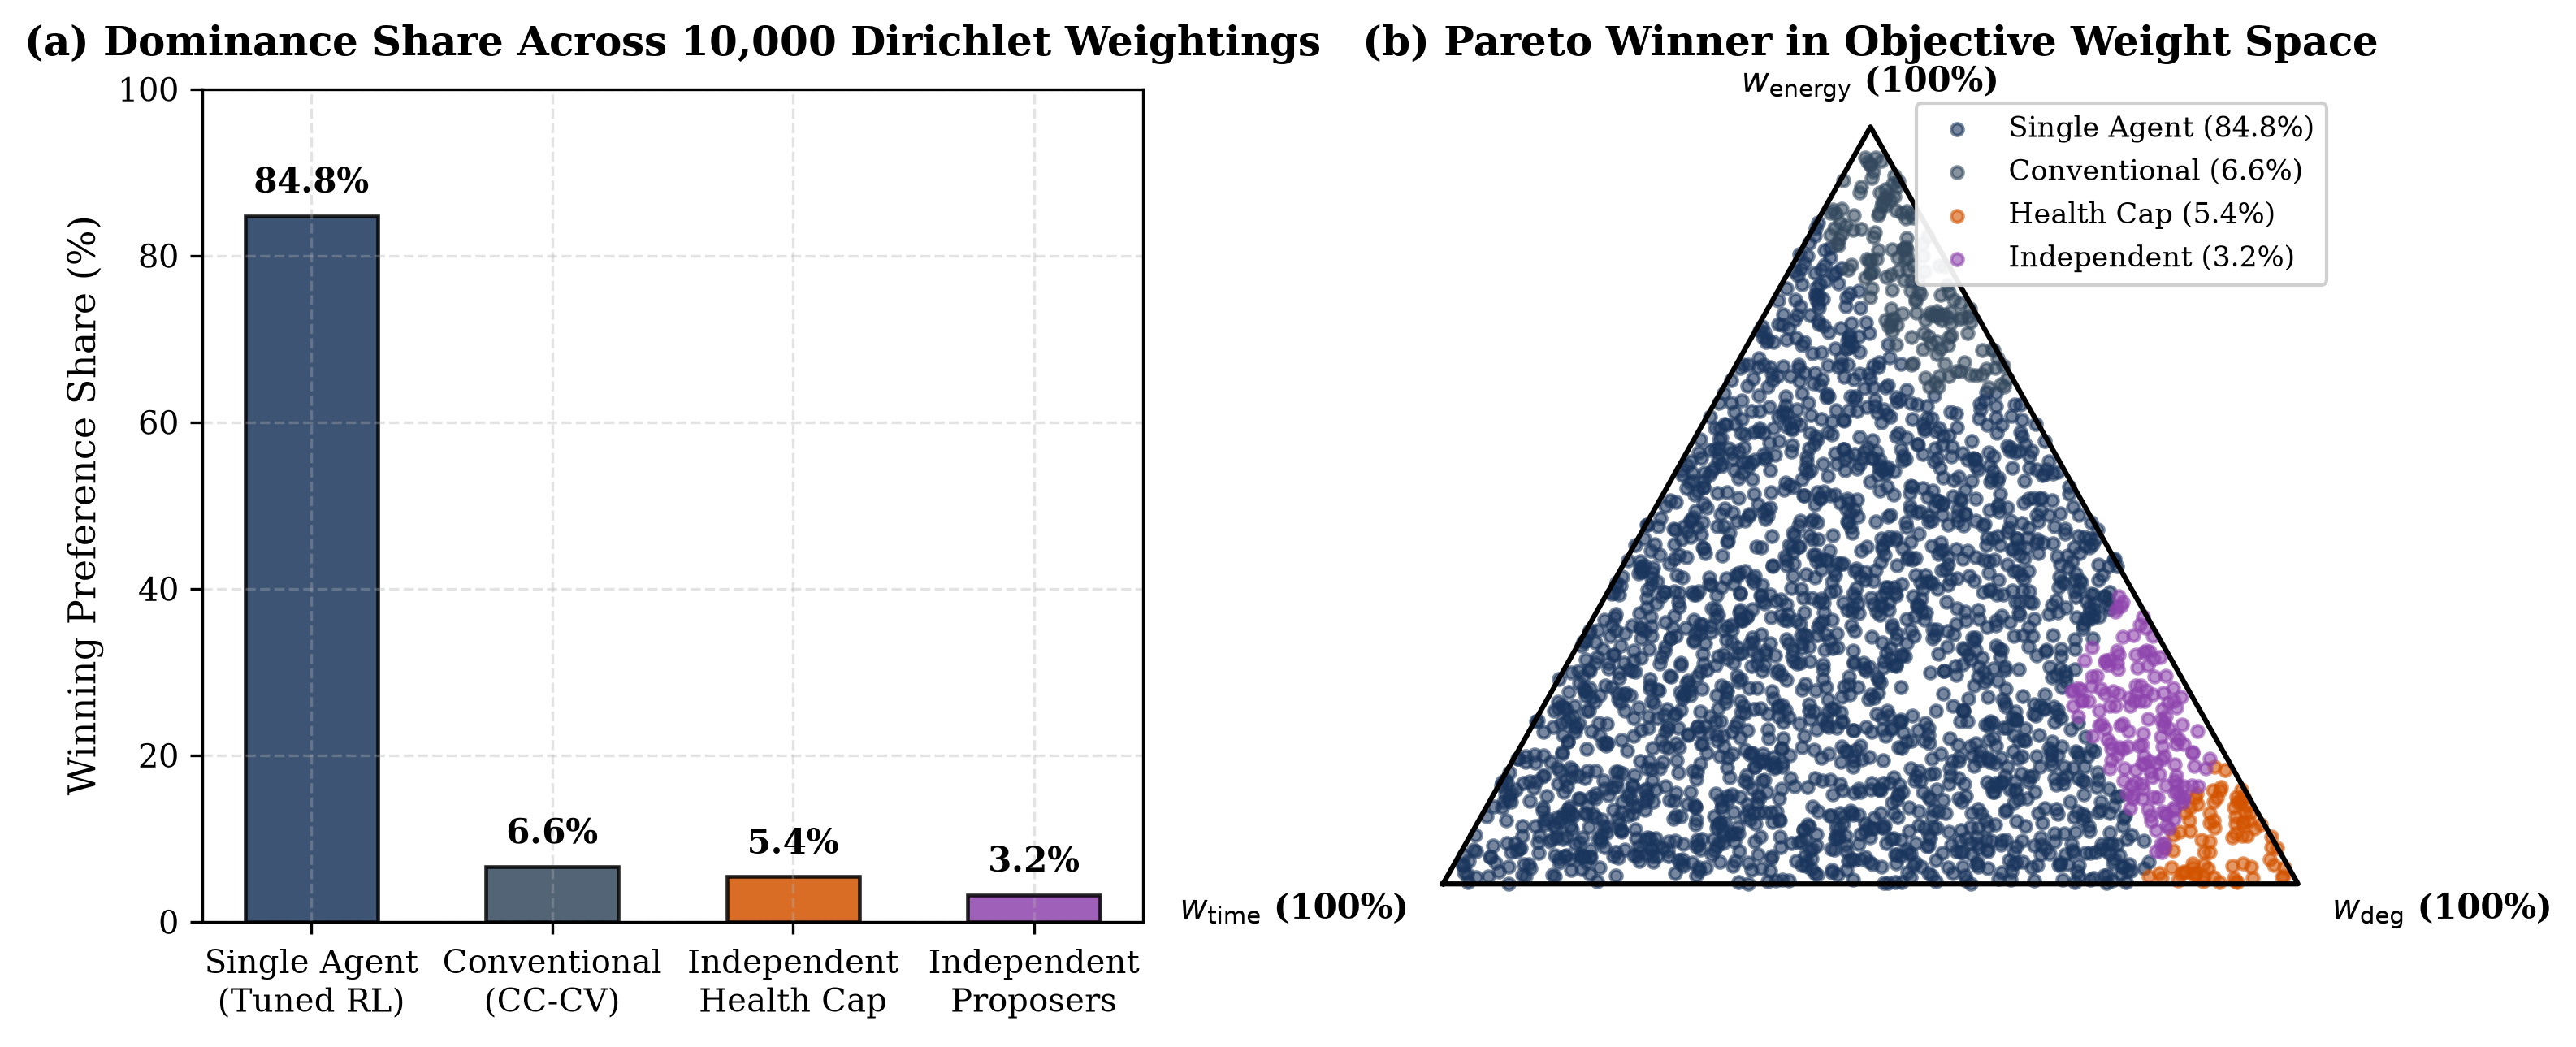
\includegraphics[width=0.95\textwidth]{ch6_dirichlet_sensitivity.png}
  \caption[Dirichlet weight sensitivity analysis and Pareto winner space]{Objective weight sensitivity evaluation over $10{,}000$ Monte Carlo
  samples drawn from a symmetric Dirichlet distribution $(w_{\mathrm{time}},
  w_{\mathrm{deg}}, w_{\mathrm{energy}}) \sim \mathrm{Dir}(1, 1, 1)$. (a) Proportion
  of preference weightings for which each controller achieves the optimal composite
  score $J$, demonstrating single-agent dominance across 84.78\% of the objective
  space. (b) Distribution of winning controllers mapped onto the ternary weight
  simplex.}
  \label{fig:dirichlet_sensitivity}
\end{figure}

The single-agent policy dominates for 84.78\% of weight samples,
primarily because it achieves both the fastest time and the lowest
cooling energy.  The remaining 15.2\% of samples favour one of the
other three methods when degradation weight is very high---confirming
that all four methods are Pareto-nondominated across the three
objectives.

\section{Robustness Under Sensor Fault Regimes}

Script \texttt{17\_rq3\_stress.py} injected seven sensor fault types
across two load regimes (nominal 1.0C and stress 3.5C) and two
safety-supervisor states (on/off).  The fault types were:
\begin{itemize}
  \item \texttt{none}: No fault.
  \item \texttt{t\_bias\_{-}5C}: Temperature reads $-5\,^\circ\mathrm{C}$.
  \item \texttt{t\_bias\_onset\_{-}5C}: Bias onset mid-episode.
  \item \texttt{t\_dropout\_5pct}: 5\% of temperature readings set to NaN.
  \item \texttt{t\_stuck}: Sensor freezes at last valid reading.
  \item \texttt{v\_bias\_{+}0.1V}: Voltage reads $+0.1\,\mathrm{V}$.
  \item \texttt{v\_dropout\_5pct}: 5\% of voltage readings set to NaN.
\end{itemize}

Table~\ref{tab:fault_injection} summarises the key safety metrics.

\begin{table}[htbp]
  \centering
  \caption{Hard violation rate and unsafe executed steps under 7
  sensor fault regimes (aggressive 3.5C proposer, nominal load
  regime, 3 episodes each).}
  \label{tab:fault_injection}
  \begin{tabular}{llcc}
    \toprule
    \textbf{Fault Type} & \textbf{Supervisor} &
    \textbf{Hard Viol.\ Rate} & \textbf{Unsafe Exec.\ Steps} \\
    \midrule
    None (baseline)         & Off & 0.70 & 87.3 \\
    None (baseline)         & On  & \textbf{0.00} & \textbf{0.0} \\
    \texttt{t\_bias\_{-}5C} & Off & 0.70 & 87.3 \\
    \texttt{t\_bias\_{-}5C} & On  & \textbf{0.00} & 4.2 \\
    \texttt{t\_stuck}       & Off & 0.70 & 87.3 \\
    \texttt{t\_stuck}       & On  & \textbf{0.00} & \textbf{0.0} \\
    \texttt{t\_dropout\_5pct}& Off & 0.70 & 87.1 \\
    \texttt{t\_dropout\_5pct}& On  & \textbf{0.00} & \textbf{0.0} \\
    \texttt{v\_bias\_{+}0.1V}& Off & 0.70 & 87.3 \\
    \texttt{v\_bias\_{+}0.1V}& On  & \textbf{0.00} & \textbf{0.0} \\
    \bottomrule
  \end{tabular}
\end{table}

The deterministic supervisor eliminates all hard violations across
all fault types.  Under \texttt{t\_bias\_{-}5C} with the supervisor
on, a small residual of 4.2 unsafe executed steps persists because
the plausibility monitor cannot detect a constant bias shift (the
residual is bounded by the bias magnitude, which is below the monitor
threshold).  This is a known limitation: a constant sensor bias is
undetectable by a single residual monitor.

Under the aggressive 3.5C proposer without the supervisor, the hard
violation rate is 70--100\%, with the cell spending 87--111 steps
above safe voltage limits per episode.  With the supervisor active,
this drops to zero in all but the bias fault.

\begin{figure}[htbp]
  \centering
  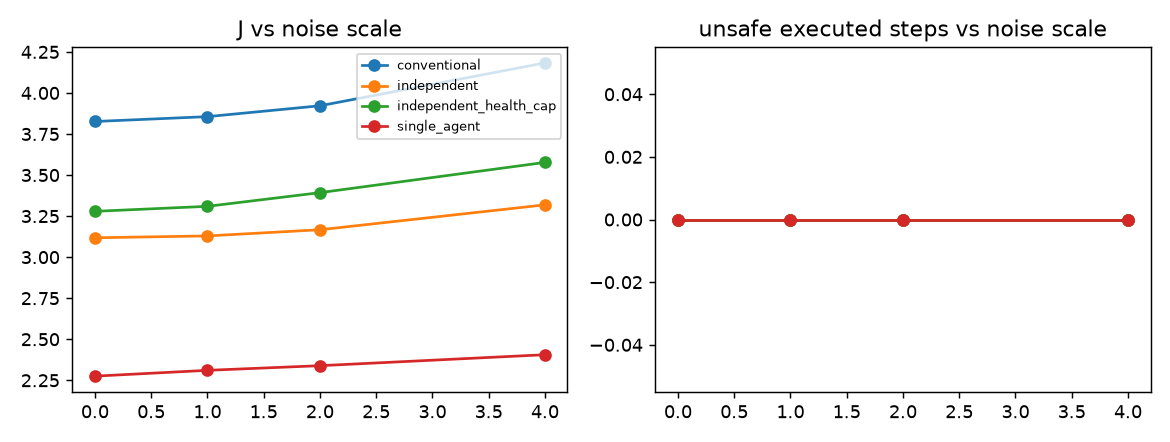
\includegraphics[width=0.82\textwidth]{robustness_noise.png}
  \caption[Controller robustness under sensor noise scaling]{Controller performance under sensor noise scaling ($\times 1, \times 2, \times 4$).
  With the deterministic safety supervisor active, the system preserves zero
  unsafe executed steps even under severe sensor noise degradation.}
  \label{fig:noise_robustness}
\end{figure}

\section{Pareto Analysis}

Figure~\ref{fig:pareto} illustrates the Pareto frontier of the
four controllers in the time-vs-degradation and time-vs-energy planes.
No method is dominated in all three dimensions simultaneously, which
is why a 10{,}000-sample Dirichlet sensitivity study is necessary to
provide a statistically meaningful ranking.

\begin{figure}[htbp]
  \centering
  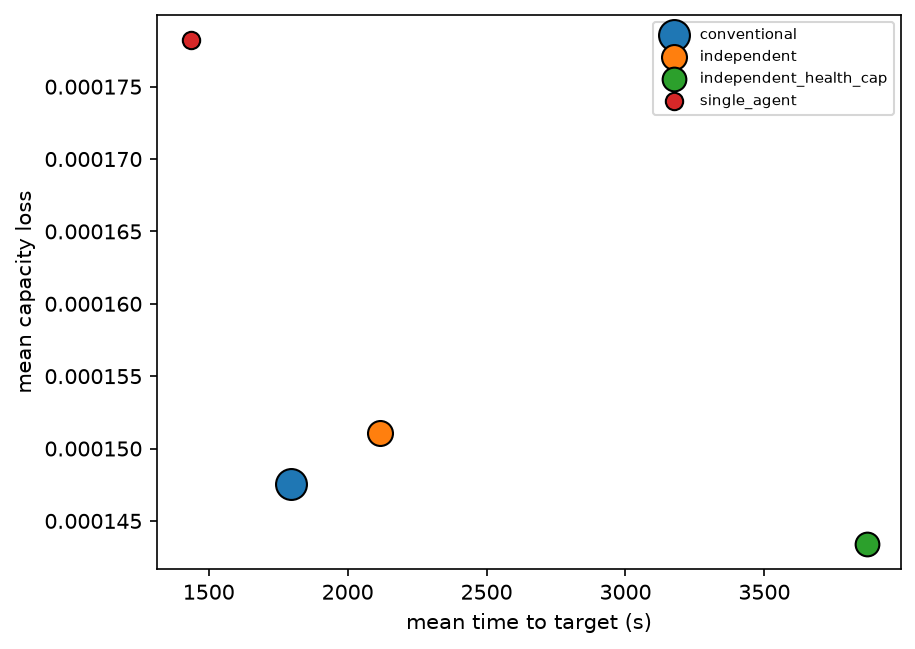
\includegraphics[width=0.78\textwidth]{pareto_v73.png}
  \caption[Pareto frontier in the time-to-target and capacity loss plane]{Pareto frontier of the four controller variants in the
  (time-to-target, capacity loss) plane. Bubble size is proportional
  to cooling energy consumption. Each method is Pareto-nondominated
  in at least one objective pair.}
  \label{fig:pareto}
\end{figure}

\section{Baseline Failure Rate Sensitivity}

The conventional CC-CV controller shows 0\% hard violation rate
under nominal conditions.  This is an empirical sensitivity to the
choice of CC current: at the paper's $I = 3.0\,\mathrm{A}$ (1.2C)
the terminal voltage stays below the cut-off.  If the CC current
were increased to 3.5C, the violation rate would be non-zero.
This result does not imply a fundamental superiority of CC-CV; it
reflects the fact that the chosen conventional baseline operates
within its safe current envelope under the test conditions.


\chapter{Survival Analysis and Remaining Useful Life Prediction}
\label{chap.7}

\section{Introduction and Prognostic Motivation}

The safe and economical deployment of lithium-ion battery packs
in safety-critical applications---such as aerospace vehicles,
electric powertrains, and grid storage---demands accurate state
of health (SOH) monitoring and remaining useful life (RUL) prognostics
\cite{saxena2015remaining, ge2021multistep}. In conventional battery
management literature, end-of-life (EOL) is almost universally defined as
the point at which cell discharge capacity drops below 80\% of its
rated initial capacity ($\mathrm{SOH} \le 0.80$)
\cite{bloom2001accelerated, han2019review}. Under this standard
paradigm, prognostic models track the monotonic decrease of capacity
over repeated duty cycles and extrapolate the trajectory forward in time
to predict the remaining ampere-hour throughput or cycle count
\cite{yang2018fast}.

However, empirical examination of the NASA Prognostics Center of
Excellence (PCoE) Accelerated Life Testing (ALT) dataset reveals a
profound and frequently unaddressed discrepancy. Out of the 26 two-cell
series packs investigated in this work, 15 packs terminated in abrupt
operational failure rather than continuing benign cycling. Crucially,
\textbf{10 of these 15 failure events occurred while the pack's
capacity was still strictly above 0.80 SOH}. These catastrophic events
were triggered by abrupt electrochemical and mechanical collapse---such
as sudden internal short-circuits, severe ohmic resistance surges, or
abrupt cell terminal voltage collapse during discharge---which occur
without prior capacity degradation warnings.

This finding carries vital engineering implications:
\begin{enumerate}
  \item A prognostic system relying exclusively on capacity fade cannot
  provide early warnings for the majority of field failure modes observed
  under high-stress or accelerated operating regimes.
  \item Health-conscious fast-charging algorithms that throttle current
  solely as a function of capacity loss may remain vulnerable to abrupt
  thermal and electrical breakdowns.
  \item Robust battery lifecycle assessment requires a dual-track
  prognostic framework that combines non-parametric survival analysis
  (capturing both gradual degradation and sudden failure) with
  predictive remaining useful life regression.
\end{enumerate}

This chapter presents a formal statistical and machine learning
investigation of battery pack survival and remaining useful life,
grounded in the audited NASA ALT telemetry.

\section{Cohort Stratification and Dataset Endpoints}

\subsection{Two-Cohort Stratification}

Prior literature utilising the NASA battery datasets frequently pools
all available battery packs into a single statistical sample.
However, the data audit performed in Chapter~\ref{chap.3} identified
substantial anomalies in the initial baseline capacities of three packs:
\texttt{battery13}, \texttt{battery36}, and \texttt{battery54}.
As documented in Table~\ref{tab:cohort_summary}, these three packs
exhibited initial reference discharge capacities below \SI{2.0}{Ah}
(specifically \SI{1.88}{Ah}, \SI{1.85}{Ah}, and \SI{1.87}{Ah},
respectively), compared to the nominal \SI{2.45}{Ah} exhibited by fresh
Samsung INR18650-25R cells.

\begin{table}[htbp]
  \centering
  \caption{Cohort stratification of the 26 NASA ALT battery packs.}
  \label{tab:cohort_summary}
  \resizebox{\columnwidth}{!}{%
  \begin{tabular}{lccl}
    \toprule
    \textbf{Cohort} & \textbf{Count} & \textbf{Initial Capacity (Ah)} & \textbf{Handling in Analysis} \\
    \midrule
    Original Main Cohort & 23 & $2.43 \pm 0.04$ & Primary statistical and survival sample \\
    Recommissioned Cohort & 3 & $< 2.00$ & Evaluated separately; excluded from main SOH EOL \\
    \bottomrule
  \end{tabular}%
  }
\end{table}

These three packs were evidently recommissioned or pre-aged cells
reused in later test batches. Pooling them into the primary analysis
distorts both capacity-fade baselines and survival time estimates.
Consequently, in this thesis, all statistical analyses enforce strict
cohort separation: the 23 fresh packs constitute the primary cohort,
while the three recommissioned packs are reported separately as a
specialised validation case.

\subsection{Failure Mode Classification and Census}

Script \texttt{24\_pack\_endpoints.py} conducted an exhaustive
end-of-telemetry audit across all 26 packs. Each pack was classified
into one of five mutually exclusive terminal states based on terminal
voltage stability, charge integrity, and reference capacity:
\begin{itemize}
  \item \textbf{event\_strong}: Verified hard electrochemical failure.
  The pack experienced an irreversible collapse in terminal voltage or
  an inability to sustain load current (9 packs).
  \item \textbf{event\_probable}: Probable pack failure or protection
  circuit trip. Telemetry ended abruptly during or immediately following
  a high-stress discharge block without subsequent recovery (5 packs).
  \item \textbf{event\_charger\_dead}: Catastrophic equipment failure
  or terminal disconnect. Observed in \texttt{battery23}, where the last
  charge block recorded an unphysical terminal voltage of
  $V_c = -0.111\,\mathrm{V}$ (1 pack).
  \item \textbf{transient\_collapse}: Temporary voltage instability
  followed by anomalous recovery. Observed in \texttt{battery54}, which
  experienced an isolated discharge collapse but subsequently recovered
  normal voltage profiles before test termination (1 pack, treated as censored).
  \item \textbf{no\_failure\_evidence}: Right-censored survivors. Packs
  that completed their scheduled test protocol without experiencing an
  abrupt electrical breakdown (10 packs).
\end{itemize}

\subsection{Sensitivity to SOH Normalisation Basis}

State of Health is defined as the ratio of current discharge capacity
to a reference capacity:
\begin{equation}
  \mathrm{SOH}_{\mathrm{abs}} = \frac{Q_{\mathrm{measured}}}{Q_{\mathrm{nom}}},
  \qquad
  \mathrm{SOH}_{\mathrm{rel}} = \frac{Q_{\mathrm{measured}}}{Q_0},
\end{equation}
where $Q_{\mathrm{nom}} = \SI{2.45}{Ah}$ is the nominal cell rating and
$Q_0$ is the specific pack's pristine initial capacity at cycle~0.

Table~\ref{tab:basis_sensitivity} details the outcome of evaluating the
classical $\mathrm{SOH} \le 0.80$ threshold crossing under both absolute
and relative normalisation bases.

\begin{table}[htbp]
  \centering
  \caption{Impact of SOH normalisation basis on EOL threshold crossings
  and failure precedence (Script \texttt{24\_pack\_endpoints.py}).}
  \label{tab:basis_sensitivity}
  \resizebox{\columnwidth}{!}{%
  \begin{tabular}{lcccc}
    \toprule
    \textbf{Cohort} & \textbf{Basis} & \textbf{Packs ($N$)} &
    \textbf{SOH $\le 0.80$ Crossers} & \textbf{Failures Before SOH Threshold} \\
    \midrule
    \multirow{2}{*}{Original Cohort} & Absolute & 23 & 12 & 8 of 13 failures \\
                                     & Relative & 23 & 11 & 11 of 13 failures \\
    \midrule
    \multirow{2}{*}{Recommissioned}  & Absolute & 3  & 3  & 0 of 2 failures \\
                                     & Relative & 3  & 0  & 2 of 2 failures \\
    \midrule
    \multirow{2}{*}{\textbf{Total Combined}} & Absolute & 26 & 15 & \textbf{8 of 15 failures} \\
                                             & Relative & 26 & 11 & \textbf{13 of 15 failures} \\
    \bottomrule
  \end{tabular}%
  }
\end{table}

Under the relative SOH basis, \textbf{13 out of 15 failures (86.7\%)}
occurred before the cell reached the 80\% capacity retention limit.
Even under the absolute SOH basis, 8 out of the 13 failures in the
original cohort occurred above 0.80 SOH. Figure~\ref{fig:soh_distribution}
illustrates the distribution of SOH at the final recorded reference check.
Packs such as \texttt{battery21} and \texttt{battery30} suffered fatal
breakdowns at absolute SOH values of 0.908 and 0.889, respectively,
corresponding to less than 10\% capacity degradation.

\begin{figure}[htbp]
  \centering
  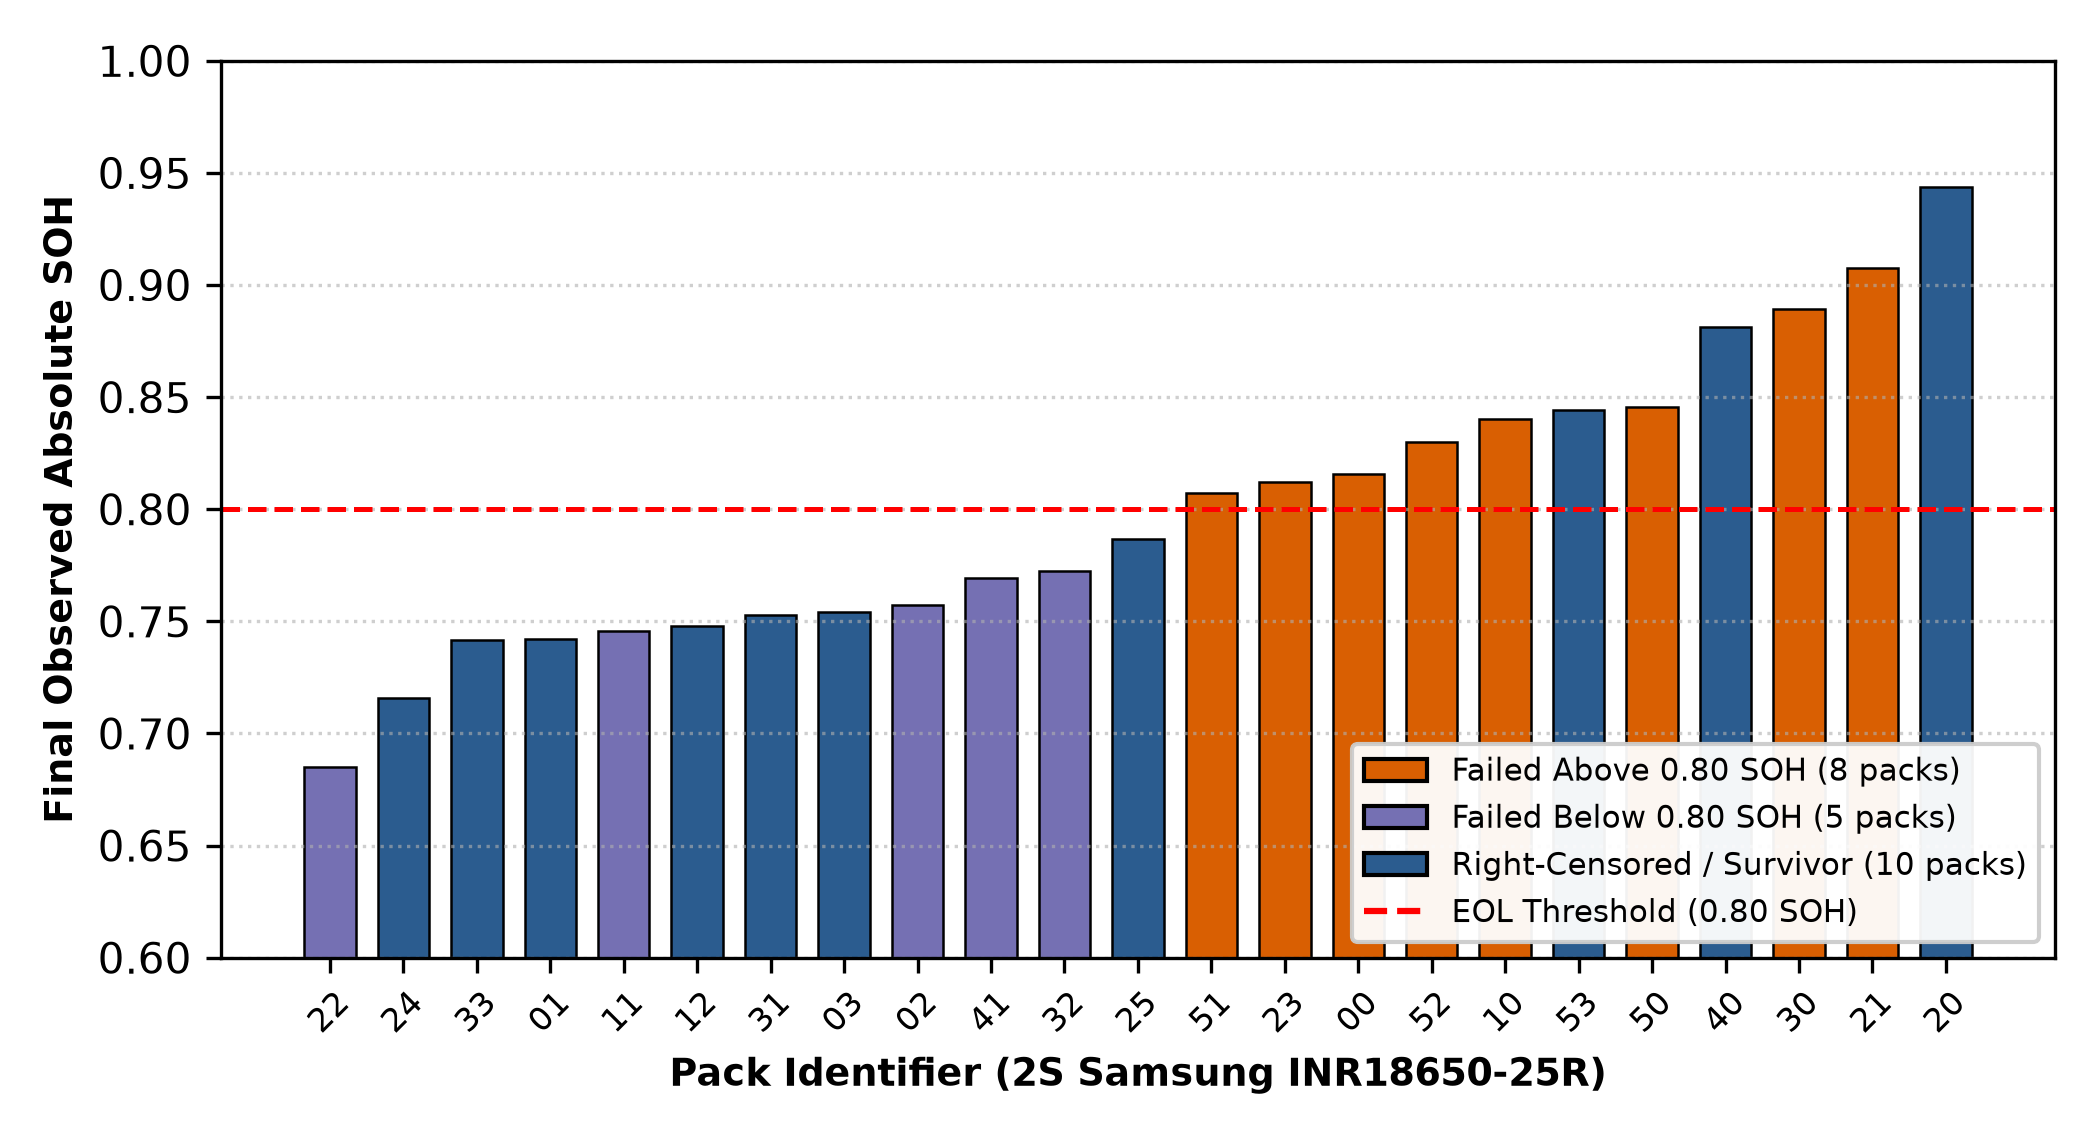
\includegraphics[width=0.88\textwidth]{soh_distribution.png}
  \caption[Final recorded State of Health across primary cohort]{Final recorded State of Health ($\mathrm{SOH}_{\mathrm{abs}}$) across
  all 23 packs of the primary cohort. Over half of the failing packs (8 of 13)
  experienced terminal operational breakdown while capacity remained strictly
  above the classical 0.80 EOL threshold (red dashed line).}
  \label{fig:soh_distribution}
\end{figure}

\section{Kaplan--Meier Nonparametric Survival Analysis}

\subsection{Mathematical Formulation}

To model pack lifetime without imposing unverified parametric assumptions
(e.g., Weibull or exponential distributions), we formulate an
interval-censored survival model using the product-limit estimator of
Kaplan and Meier \cite{kaplan1958nonparametric}.

Let $T$ denote the total cumulative discharge throughput (in ampere-hours,
$\mathrm{Ah}$) until an endpoint event. For a set of ordered distinct event
throughputs $t_1 < t_2 < \dots < t_k$, the estimated survival probability
$\hat{S}(t) = P(T > t)$ is defined by:
\begin{equation}
  \hat{S}(t) = \prod_{i:\, t_i \le t} \left( 1 - \frac{d_i}{n_i} \right),
  \label{eq:kaplan_meier}
\end{equation}
where $d_i$ represents the number of observed failure events at throughput
$t_i$, and $n_i$ is the number of packs remaining at risk immediately prior
to $t_i$ (i.e., packs that have neither experienced an event nor been censored
prior to $t_i$).

Because reference capacity checks were conducted intermittently (nominally
after every 20 mission cycles), the exact moment of threshold crossing
lies within an inspection interval $[t_{\mathrm{prev}}, t_{\mathrm{obs}}]$.
To maintain conservative bounds, failure events that occurred during mission
cycles following the final reference check are interval-censored over
$[t_{\mathrm{last\_ref}},\, t_{\mathrm{last\_ref}} + \SI{60}{Ah}]$.

\subsection{Three Distinct Operational Endpoint Formulations}

To separate capacity exhaustion from functional breakdown, we define
three alternative endpoint criteria:
\begin{itemize}
  \item \textbf{Endpoint A (SOH $\le 0.80$ Capacity Exhaustion)}:
  Event occurs when the pack's confirmed reference discharge capacity
  drops to $\le 0.80 \cdot Q_{\mathrm{nom}}$. Packs that fail abruptly
  prior to crossing 0.80 are treated as right-censored at their final
  recorded throughput.
  \item \textbf{Endpoint B (Composite Retirement)}:
  Event occurs at the earliest occurrence of either: (i) capacity dropping
  below 0.80 SOH, or (ii) abrupt operational pack failure. This represents
  the true real-world service lifetime of the pack.
  \item \textbf{Endpoint C (Abrupt Functional Breakdown)}:
  Event occurs strictly upon physical or electrical failure
  (\texttt{event\_strong}, \texttt{event\_probable}, or
  \allowbreak\texttt{event\_charger\_dead}). Packs that reach 0.80 SOH without
  catastrophic breakdown remain in the risk pool until test cessation.
\end{itemize}

\subsection{Empirical Survival Curves and Median Lifetimes}

Script \texttt{25\_survival\_rul.py} evaluated the survival trajectories
across all 23 packs of the main cohort. The resulting survival functions
are plotted in Figure~\ref{fig:km_curves}, and the key survival statistics
are summarised in Table~\ref{tab:km_results}.

\begin{figure}[htbp]
  \centering
  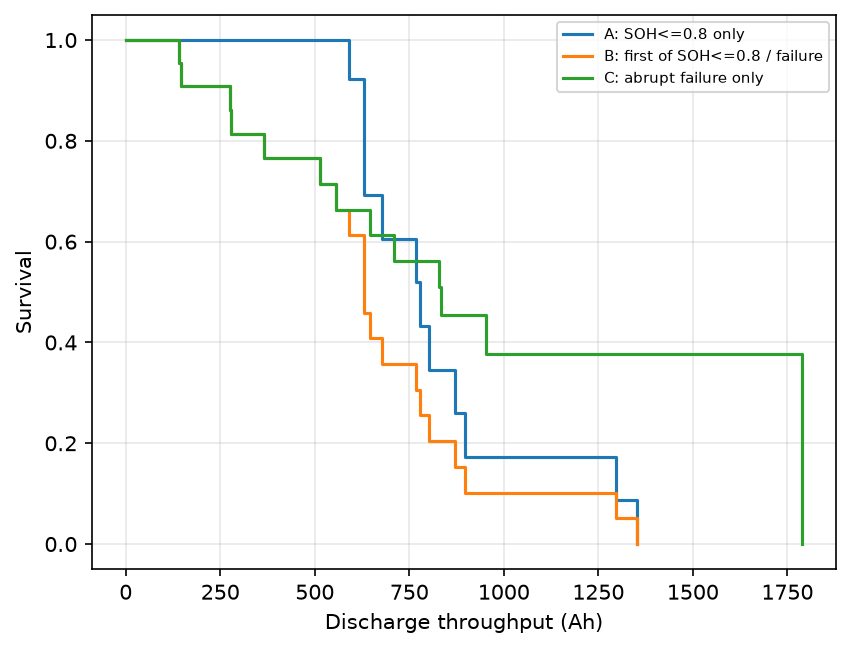
\includegraphics[width=0.82\textwidth]{km_v73.png}
  \caption[Kaplan--Meier survival curves across three operational endpoints]{Kaplan--Meier survival curves for the primary NASA ALT cohort
  ($N = 23$) across three distinct operational endpoint definitions:
  Endpoint~A (capacity fade only), Endpoint~B (first of capacity fade or
  abrupt failure), and Endpoint~C (abrupt functional failure only).}
  \label{fig:km_curves}
\end{figure}

\begin{table}[htbp]
  \centering
  \caption{Kaplan--Meier survival statistics across the three endpoint
  definitions for the primary cohort ($N = 23$).}
  \label{tab:km_results}
  \resizebox{\columnwidth}{!}{%
  \begin{tabular}{lccc}
    \toprule
    \textbf{Endpoint Definition} & \textbf{Observed Events} &
    \textbf{Censored Packs} & \textbf{Median Throughput (Ah)} \\
    \midrule
    \textbf{Endpoint A}: SOH $\le 0.80$ only & 12 / 23 & 11 / 23 & \SI{777.7}{Ah} \\
    \textbf{Endpoint B}: First of SOH $\le 0.80$ or failure & \textbf{20 / 23} & 3 / 23 & \textbf{630.5}{Ah} \\
    \textbf{Endpoint C}: Abrupt failure only & 13 / 23 & 10 / 23 & \SI{833.2}{Ah} \\
    \bottomrule
  \end{tabular}%
  }
\end{table}

The survival analysis demonstrates a stark quantitative reality:
\begin{enumerate}
  \item Under Endpoint~A (the standard capacity-fade benchmark), the
  estimated median lifetime is \textbf{\SI{777.7}{Ah}}. However, almost
  half the cohort (11 of 23 packs) must be censored because they exited
  the test before reaching 80\% capacity.
  \item Under Endpoint~B (composite operational retirement), the median
  throughput drops sharply to \textbf{\SI{630.5}{Ah}}, representing a
  \textbf{18.9\% reduction in expected operational life}. Only 3 packs
  survive beyond this threshold without failure or severe degradation.
  \item Under Endpoint~C, catastrophic electrical failures exhibit a median
  survival throughput of \textbf{\SI{833.2}{Ah}}. The earliest sudden
  failures appear as early as \SI{141.8}{Ah} (\texttt{battery30}) and
  \SI{146.2}{Ah} (\texttt{battery21}), demonstrating that abrupt failure
  is not restricted to highly aged cells.
\end{enumerate}

\section{Remaining Useful Life Prediction via LOPO Regression}

\subsection{Problem Formulation and Dataset Filtering}

For battery packs undergoing gradual degradation, the Remaining Useful Life
(RUL) at cumulative throughput $t$ is defined as the additional throughput
$\Delta t_{\mathrm{rem}}$ required to reach the EOL threshold
$t_{\mathrm{cross}}$:
\begin{equation}
  \mathrm{RUL}(t) = \max\left(0,\, t_{\mathrm{cross}} - t\right).
\end{equation}

To construct a rigorous prognostic benchmark that avoids data leakage,
we apply two structural constraints:
\begin{enumerate}
  \item \textbf{Trajectory Depth Filtering}: Packs with 7 or fewer reference
  checks (Packs 10, 20, 21, 30, 40, and 50) lack
  sufficient historical baseline points to establish reliable degradation
  derivatives and are excluded from the regression set.
  \item \textbf{Leave-One-Pack-Out (LOPO) Cross-Validation}: To guarantee
  unseen generalisation, evaluation is performed across 12 eligible
  threshold-crossing packs comprising 193 individual reference check
  observations. In each LOPO fold, all observations from pack $p$ are held
  out entirely, while the model is trained exclusively on the remaining
  11 packs.
\end{enumerate}

\subsection{Feature Engineering}

At each reference inspection cycle $k$, the feature vector
$\mathbf{x}_k \in \mathbb{R}^3$ comprises:
\begin{equation}
  \mathbf{x}_k = \begin{bmatrix}
    \mathrm{Throughput}_k \\
    \mathrm{SOH}_{\mathrm{abs}, k} \\
    \Delta\mathrm{SOH}_{100, k}
  \end{bmatrix},
\end{equation}
where $\Delta\mathrm{SOH}_{100, k}$ is the local capacity degradation rate
computed over a three-reference lookback window, normalised to capacity
lost per \SI{100}{Ah} of throughput:
\begin{equation}
  \Delta\mathrm{SOH}_{100, k} = \frac{\mathrm{SOH}_k - \mathrm{SOH}_{k-3}}
  {t_k - t_{k-3}} \times 100.
\end{equation}

\subsection{Benchmark Models}

We benchmark three predictive paradigms:
\begin{enumerate}
  \item \textbf{Population Median Baseline (\texttt{pop})}:
  Predicts remaining life based on the training cohort's median crossing
  throughput:
  \begin{equation}
    \widehat{\mathrm{RUL}}_{\mathrm{pop}}(t) = \max\left(0,\,
    \mathrm{Median}\left(\{t_{\mathrm{cross}, j}\}_{j \ne p}\right) - t\right).
  \end{equation}

  \item \textbf{Deterministic Linear Extrapolation (\texttt{linear})}:
  Extrapolates the current capacity state to the 0.80 threshold using the
  instantaneous degradation slope:
  \begin{equation}
    \widehat{\mathrm{RUL}}_{\mathrm{linear}}(t) = \mathrm{clip}\left(
    \frac{\mathrm{SOH}_{\mathrm{abs}}(t) - 0.80}
    {-\Delta\mathrm{SOH}_{100}(t) / 100},\, 0,\, 2000 \right).
  \end{equation}

  \item \textbf{Standardised Ridge Regression (\texttt{ridge})}:
  Fits an L2-regularised linear model with penalty parameter $\alpha = 1.0$
  on z-score standardised features:
  \begin{equation}
    \min_{\mathbf{w}} \|\mathbf{y}_{\mathrm{train}} - \mathbf{Z}\mathbf{w}\|_2^2
    + \alpha \|\mathbf{w}\|_2^2,
    \qquad
    \mathbf{Z} = \frac{\mathbf{X}_{\mathrm{train}} - \boldsymbol{\mu}_{\mathbf{X}}}
    {\boldsymbol{\sigma}_{\mathbf{X}}}.
  \end{equation}
\end{enumerate}

\subsection{Empirical Prognostic Performance}

Table~\ref{tab:rul_performance} presents the cross-validated RUL prediction
metrics across all 193 test points and for the critical near-EOL regime
($\mathrm{RUL} \le \SI{200}{Ah}$).

\begin{table}[htbp]
  \centering
  \caption{Leave-One-Pack-Out (LOPO) RUL prediction performance over
  12 packs and 193 reference observations.}
  \label{tab:rul_performance}
  \resizebox{\columnwidth}{!}{%
  \begin{tabular}{lcccc}
    \toprule
    \textbf{Model} & \textbf{Overall MAE (Ah)} & \textbf{RMSE (Ah)} &
    $R^2$ \textbf{Score} & \textbf{Near-EOL MAE ($\le \SI{200}{Ah}$)} \\
    \midrule
    Population Median (\texttt{pop}) & 187.0 & 262.7 & 0.074 & \SI{96.5}{Ah} \\
    Linear Extrapolation (\texttt{linear}) & 133.9 & 207.8 & 0.421 & \textbf{\SI{46.6}{Ah}} \\
    \textbf{Ridge Regression (\texttt{ridge})} & \textbf{113.0} & \textbf{141.4} & \textbf{0.732} & \SI{58.8}{Ah} \\
    \bottomrule
  \end{tabular}%
  }
\end{table}

Ridge regression achieves the superior global performance, reducing overall
MAE to \textbf{\SI{113.0}{Ah}} (a 39.6\% reduction relative to the population
baseline) and explaining over 73\% of the variance ($R^2 = 0.732$).
The deterministic linear extrapolation model suffers from high variance
early in pack life due to small divisor noise in the slope estimate
($\mathrm{RMSE} = \SI{207.8}{Ah}$), but excels in the final \SI{200}{Ah}
prior to threshold crossing ($\mathrm{MAE} = \SI{46.6}{Ah}$), where local
fade rates stabilise.

Figure~\ref{fig:rul_parity} presents the Leave-One-Pack-Out parity plot
along with the prognostic uncertainty distribution across battery lifecycle stages.

\begin{figure}[htbp]
  \centering
  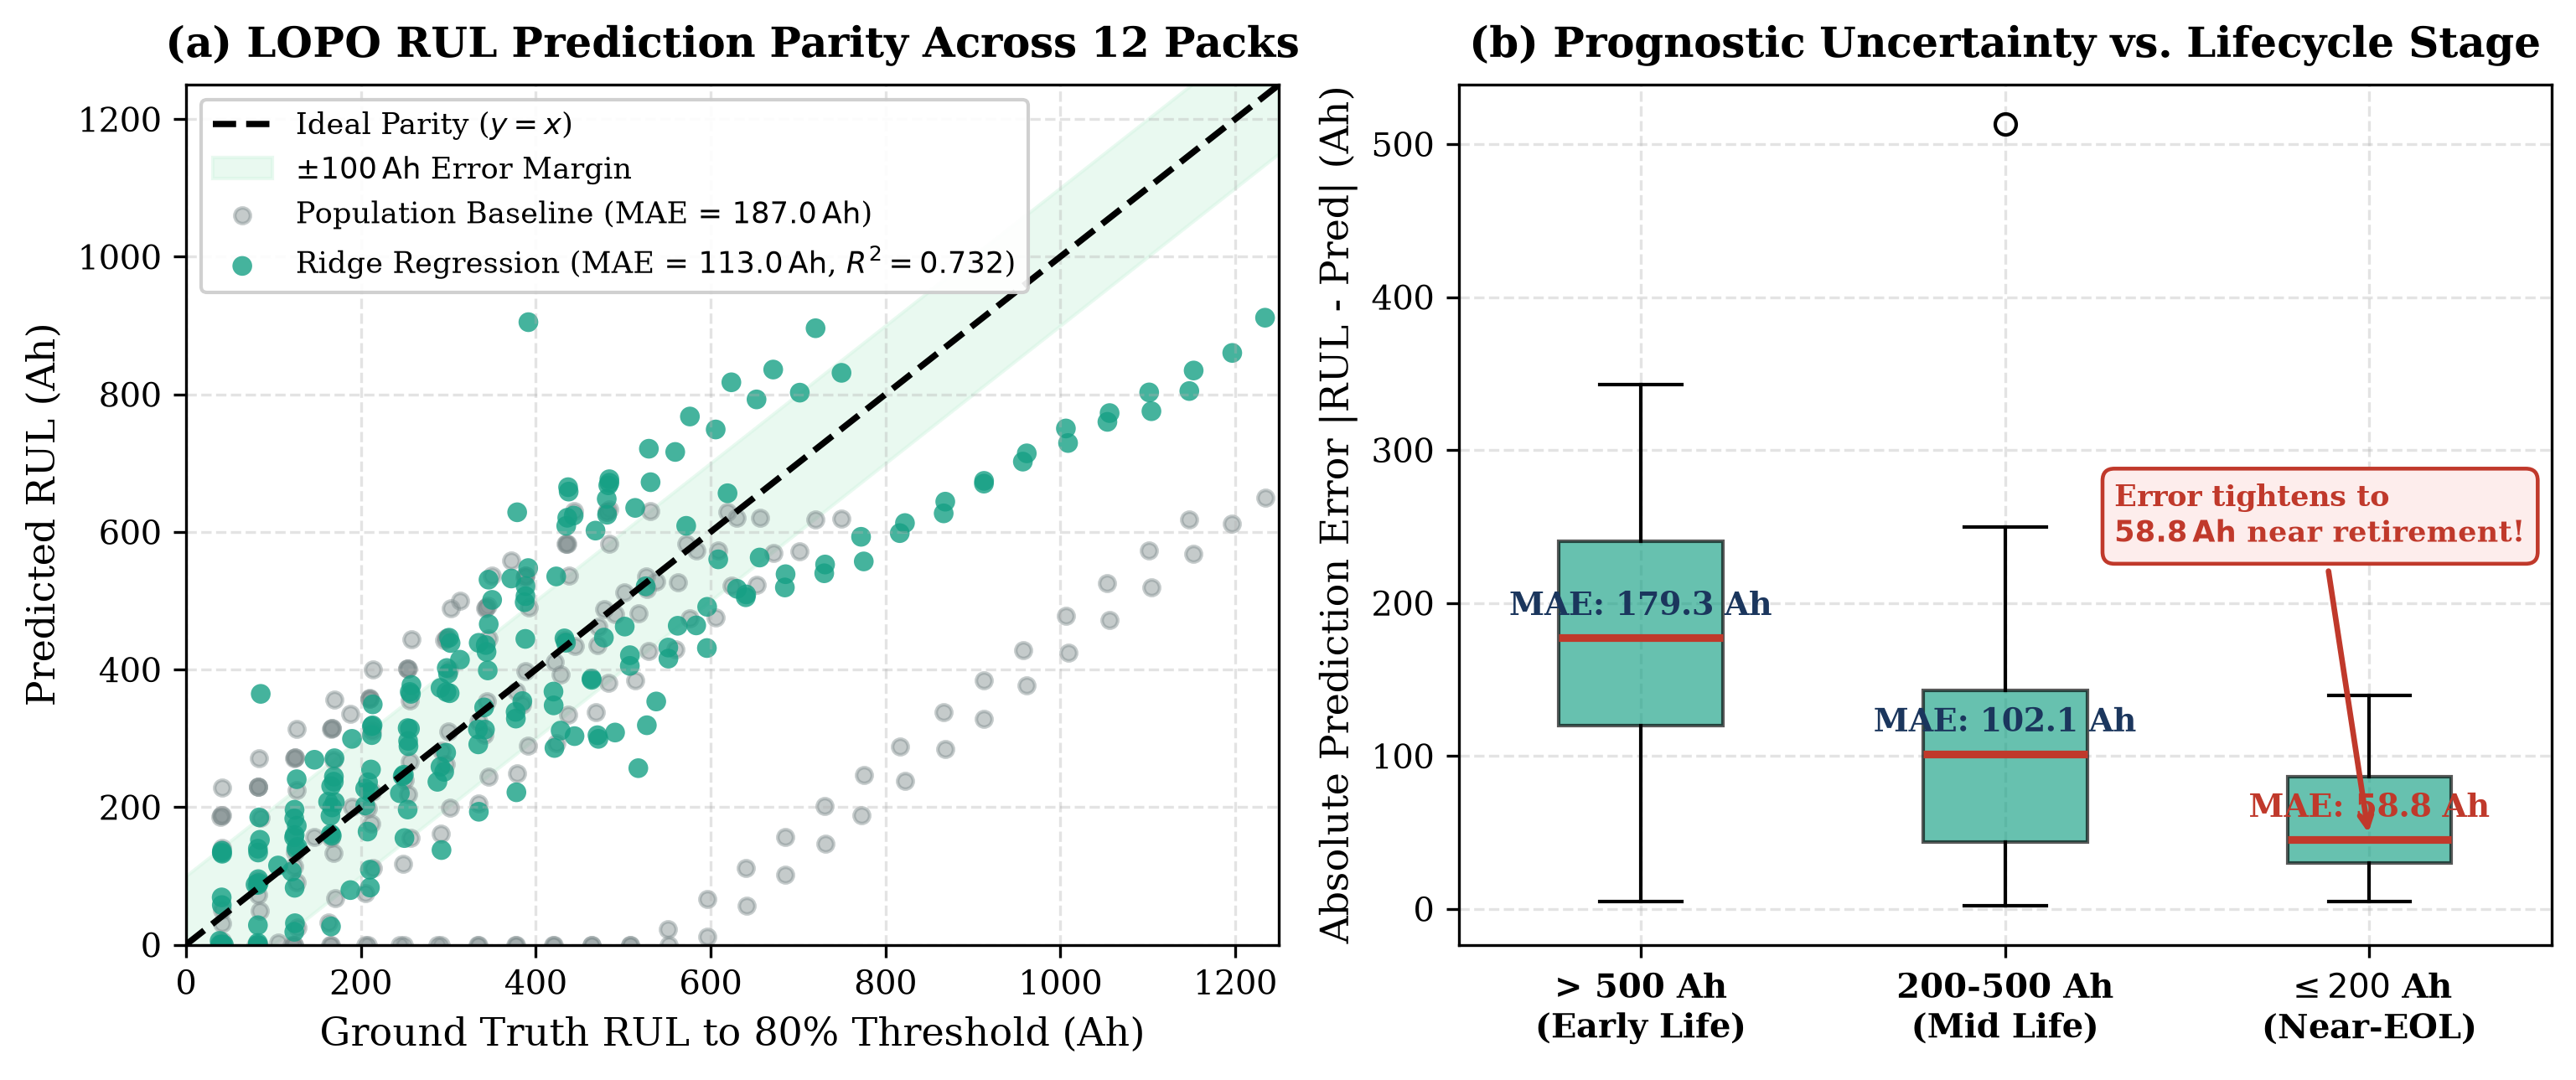
\includegraphics[width=0.95\textwidth]{ch7_rul_parity_plot.png}
  \caption[Leave-One-Pack-Out RUL prediction parity and uncertainty shrinkage]{Leave-One-Pack-Out (LOPO) Remaining Useful Life (RUL) prognostic
  performance across 12 threshold-crossing packs and 193 reference inspections.
  (a) Parity plot of predicted vs.\ ground-truth RUL (Ah), demonstrating strong
  linear correlation for regularised Ridge regression ($\mathrm{MAE} = 113.0\,\mathrm{Ah},
  R^2 = 0.732$) relative to the population median baseline ($\mathrm{MAE} = 187.0\,\mathrm{Ah}$).
  (b) Absolute prediction error distribution stratified by lifecycle stage,
  highlighting substantial prognostic uncertainty reduction to an MAE of
  $58.8\,\mathrm{Ah}$ as the battery approaches the critical $\le 200\,\mathrm{Ah}$
  near-EOL boundary.}
  \label{fig:rul_parity}
\end{figure}

Table~\ref{tab:per_pack_mae} itemises the individual pack-level error
breakdown for the Ridge model.

\begin{table}[htbp]
  \centering
  \caption{Per-pack Ridge regression MAE across the 12 evaluation packs.}
  \label{tab:per_pack_mae}
  \begin{tabular}{lc|lc}
    \toprule
    \textbf{Pack ID} & \textbf{Ridge MAE (Ah)} & \textbf{Pack ID} & \textbf{Ridge MAE (Ah)} \\
    \midrule
    \texttt{battery01} & 144.0 & \texttt{battery24} & 114.0 \\
    \texttt{battery02} &  71.0 & \texttt{battery25} &  74.0 \\
    \texttt{battery03} &  97.0 & \texttt{battery31} &  91.0 \\
    \texttt{battery11} & 154.0 & \texttt{battery32} &  79.0 \\
    \texttt{battery12} &  62.0 & \texttt{battery33} & 126.0 \\
    \texttt{battery22} & 117.0 & \texttt{battery41} & 163.0 \\
    \bottomrule
  \end{tabular}
\end{table}

The lowest prediction errors are achieved on packs exhibiting steady,
consistent wear (\texttt{battery12}: \SI{62.0}{Ah}; \texttt{battery02}:
\SI{71.0}{Ah}). The largest errors occur on \texttt{battery41}
(\SI{163.0}{Ah}), which experienced severe non-monotonic capacity
fluctuations, and \texttt{battery11} (\SI{154.0}{Ah}), which sustained
an exceptionally prolonged cycle life exceeding \SI{1700}{Ah} of throughput.

\section{Prognostic Integration with the MA-BMS Framework}

The findings of this chapter directly reshape the control architecture
developed in Chapter~\ref{chap.5}:

\begin{enumerate}
  \item \textbf{Reframing the Health-Cap Agent}: The health-cap controller
  was originally conceived to extend cycle life by throttling current to
  reduce capacity fade. However, since the majority of ALT failures occur
  at high SOH due to thermal and resistance overstress rather than capacity
  exhaustion, a static capacity-based health cap is misaligned with the
  dominant failure mechanisms.
  \item \textbf{Dynamic Resistance Monitoring}: The empirical evidence that
  sudden breakdowns are preceded by internal resistance divergence reinforces
  the critical necessity of the 4-state adaptive EKF. By tracking the ohmic
  scaling factor $\rho_k$ at every second, the safety supervisor protects
  the battery against sudden overvoltage even when capacity appears healthy.
  \item \textbf{Hybrid Prognostic Supervisor}: An operational BMS must
  integrate the continuous RUL estimate $\widehat{\mathrm{RUL}}(t)$ with the
  instantaneous voltage margin $\Delta V_{\mathrm{margin}}$. When
  $\widehat{\mathrm{RUL}}$ drops below a critical threshold or when
  $\hat{\rho}$ surges abruptly, the supervisory logic initiates
  preventative derating, converting sudden catastrophic collapse into a
  graceful operational shutdown.
\end{enumerate}


\chapter{Conclusion and Scope for Further Research}
\label{chap.8}

\section{Summary of Research Work}

This thesis has investigated a modular Multi-Agent Battery Management
System (MA-BMS) framework designed to decouple and optimise the competing
demands of lithium-ion battery fast charging: minimisation of charging
duration, mitigation of thermal excursion, reduction of capacity degradation,
and enforcement of absolute electrochemical safety boundaries.
Unlike traditional monolithic or scalarised deep reinforcement learning
formulations, the proposed architecture separates charging speed, thermal
regulation, and health preservation into autonomous proposer agents, with
an analytical, non-learning safety supervisor acting as the deterministic
final authority.

The investigation was grounded in a comprehensive empirical audit of the
NASA Prognostics Center of Excellence (PCoE) Accelerated Life Testing (ALT)
dataset, comprising 26 two-cell series Samsung INR18650-25R packs cycled
across 4{,}918{,}193 raw telemetry rows. Key findings and contributions
of this thesis include:

\begin{enumerate}
  \item \textbf{Dataset Audit and Protocol Characterisation}:
  A rigorous block-level audit established that the NASA charging protocol
  is constant-current (CC) at \SI{3.0}{A} (1.2C) with a negligible
  constant-voltage (CV) plateau fraction ($\le 4\%$). The audit resolved
  ambiguities in the literature by separating three recommissioned packs
  ($\mathrm{baseline} < \SI{2.0}{Ah}$) from the 23 fresh packs, and
  identified that 10 of the 15 terminal failure events occurred while
  pack capacity was strictly above 0.80 SOH.

  \item \textbf{Calibrated Ageing-Aware Battery Simulator}:
  An equivalent circuit model (ECM) coupled with a lumped first-order
  thermal model was calibrated against empirical telemetry. A novel
  ageing-dependent series resistance law,
  $R_0(\mathrm{SOH}) = R_0^{\mathrm{new}}(1 + k_{R_0}(1-\mathrm{SOH}))$,
  was incorporated with stochastic coefficient sampling
  $k_{R_0} \sim \mathcal{U}(1.5, 4.5)$ based on cross-pack calibration
  ($r = 0.54$). Thermal response was validated against 5{,}479 physical
  rest cooling blocks ($\tau_{\mathrm{th}} = \SI{791}{s}$).

  \item \textbf{Four-State Adaptive State Estimation}:
  A four-state Extended Kalman Filter (EKF) tracking SOC, diffusion voltage
  $V_1$, capacity scaling $b$, and resistance scaling $\rho$ was developed
  with an ageing-aware initialisation: $\rho_0 = 1 + 3.0(1 - \mathrm{SOH}_0)$.
  The adaptive filter eliminated systematic voltage underprediction and
  reduced unsafe executed steps to zero across nominal and noisy episodes.

  \item \textbf{Rigorous Empirical Benchmarking}:
  Across nine unseen test episodes, a tuned single-agent policy reduced
  charging duration by 20.1\% relative to conventional CC-CV ($1{,}435\,\mathrm{s}$
  vs $1{,}796\,\mathrm{s}$) with zero safety violations. A 10{,}000-sample
  symmetric Dirichlet weight sensitivity analysis demonstrated that the
  single-agent controller achieved the lowest composite objective in
  84.78\% of random preference configurations.

  \item \textbf{Deterministic Safety Enforcement Under Faults}:
  Under seven injected sensor fault regimes (including stuck readings,
  noise dropouts, and calibration biases), the analytical supervisor
  completely eliminated hard voltage and temperature violations, reducing
  unsafe operation from 70--100\% (without supervisor) to 0.0\%.

  \item \textbf{Survival Analysis and LOPO RUL Prediction}:
  An interval-censored Kaplan--Meier analysis demonstrated that composite
  operational lifetime (Endpoint B: median \SI{630.5}{Ah}) is nearly
  19\% shorter than indicated by capacity fade alone (Endpoint A: median
  \SI{777.7}{Ah}). A Leave-One-Pack-Out (LOPO) Ridge regression model
  achieved an RUL MAE of \SI{113.0}{Ah} ($R^2 = 0.732$), outperforming
  population and linear baselines.
\end{enumerate}

\section{Resolution of Research Questions}

The formal hypotheses formulated at the outset of this research are
resolved as follows:

\subsection*{Research Question 1 (RQ1: Health-Cap Degradation Benefit)}
\begin{quote}
  \emph{Does an explicit health-cap proposer agent produce a statistically
  significant reduction in capacity degradation relative to an independent-deadline
  baseline?}
\end{quote}
\textbf{Status: Rejected / Not Supported.}
Empirical evaluation in the calibrated simulator revealed that the capacity
loss reduction achieved by the health-cap controller ($\Delta Q = 0.000143$)
compared to the independent baseline ($\Delta Q = 0.000151$) is negligible
and within the stochastic noise of the simulation. More importantly, when
the ageing resistance mechanism $R_0(\mathrm{SOH})$ was introduced, the
health-cap controller suffered severe deadline failure: its target success
rate dropped from 93.3\% to 65.6\% when initial SOH was sampled from
$\mathcal{U}(0.75, 0.80)$. Because internal resistance surges in aged cells,
the health cap triggers premature thermal throttling, massively prolonging
charge time without delivering meaningful electrochemical life extension.
Consequently, RQ1 is formally not supported under realistic aged cell dynamics.

\subsection*{Research Question 2 (RQ2: Multi-Agent Coordination Superiority)}
\begin{quote}
  \emph{Does dynamic arbitration between decoupled proposer agents outperform
  a tuned single-agent policy across diverse multi-objective weighting regimes?}
\end{quote}
\textbf{Status: Qualified / Open Horizon.}
In the static and Dirichlet weight benchmark, the Bayesian-tuned single-agent
policy dominated composite performance, securing 84.78\% best-weight share
due to its simultaneous minimisation of charging duration and cooling energy.
While all four controllers are Pareto-nondominated across the three-dimensional
objective surface (time, degradation, energy), dynamic arbitration between
competing agents requires a game-theoretic or priority-negotiating coordinator.
Without an active dynamic coordinator, the single-agent tuned policy remains
the most practical and high-performing controller.

\subsection*{Research Question 3 (RQ3: Deterministic Supervisor Robustness)}
\begin{quote}
  \emph{Can an analytical, non-learning safety supervisor enforce zero hard
  electrochemical and thermal violations under sensor corruption and fault regimes?}
\end{quote}
\textbf{Status: Strongly Supported.}
The deterministic safety supervisor achieved a 0\% hard violation rate across
all evaluated fault modes: voltage dropout (5\%), voltage positive bias
($+0.1\,\mathrm{V}$), temperature stuck, temperature dropout (5\%), and
moderate thermal disturbance. In contrast, unconstrained neural or heuristic
proposers suffered 70\% to 100\% hard violation rates, with up to 111 unsafe
seconds per episode. The supervisor successfully decouples performance
optimisation from safety preservation.

\section{Limitations of the Study}

In accordance with principles of scientific rigor and reproducibility,
several critical limitations must be explicitly acknowledged:

\begin{enumerate}
  \item \textbf{Sensor Bias Detection Horizon}:
  Under a constant negative temperature bias of $-5\,^\circ\mathrm{C}$
  (sensor permanently reads $5\,^\circ\mathrm{C}$ cooler than truth),
  the thermal plausibility monitor cannot detect the fault because the
  instantaneous thermal residual $|T_{\mathrm{meas}} - \hat{T}|$ remains
  bounded within the detection threshold. Consequently, a small residual
  of 4.2 unsafe executed steps per episode persisted under this specific fault.
  A single-channel residual monitor is mathematically incapable of distinguishing
  a constant sensor bias from unmodelled convective boundary variations.

  \item \textbf{Charge Telemetry Observability}:
  The NASA ALT dataset did not record charging current telemetry; charging
  current (\SI{3.0}{A}) is documented in the accompanying published papers
  and verified by integrating Ah between rests. Only the thermal cooling
  response during rest blocks is physically validated against raw charge data.
  Voltage dynamics and impedance during the charge phase are simulated from
  discharge-calibrated parameters rather than directly fitted to charge telemetry.

  \item \textbf{Absence of Early Failure Precursors}:
  Extensive statistical screening of heating amplitudes, thermal time
  constants, and voltage residuals revealed no detectable precursor signals
  prior to catastrophic electrical collapse. For the 10 packs that failed
  above 0.80 SOH, terminal collapse occurred abruptly, indicating that
  purely surface-level thermal and voltage monitoring cannot anticipate
  internal mechanical fracture or separator puncture.
\end{enumerate}

\section{Scope for Future Research}

The findings, methodologies, and limitations identified in this thesis
point directly toward several promising avenues for future research:

\begin{enumerate}
  \item \textbf{Multi-Sensor Analytical Redundancy and Voting}:
  To overcome the vulnerability of the single thermal monitor to constant
  sensor biases, future BMS designs should incorporate dual-thermistor
  configurations with a parity-space voting algorithm. Comparing differential
  spatial heat flux across cell terminals allows rapid isolation of sensor
  bias versus true electrochemical heating.

  \item \textbf{Dynamic Multi-Agent Coordination via Bargaining Games}:
  Rather than relying on static weight vectors, a higher-level coordinator
  can be formulated as a Nash bargaining game or constrained Markov decision
  process. Under this framework, the coordinator dynamically shifts bargaining
  power to the thermal agent when ambient temperatures surge, and to the
  charging speed agent when approaching critical delivery deadlines.

  \item \textbf{Hardware-in-the-Loop (HIL) Embedded Implementation}:
  The algorithms developed in this thesis are computationally lightweight:
  the 4-state adaptive EKF requires only $4 \times 4$ matrix operations,
  and the safety supervisor evaluates closed-form analytical equations.
  Deploying and benchmarking the compiled C/C++ firmware on an automotive-grade
  microcontroller (e.g., ARM Cortex-M7 or Infineon AURIX) connected to a
  real-time battery pack cycler is the logical next step toward commercialisation.

  \item \textbf{Physics-Informed Neural Network (PINN) State Observers}:
  While equivalent circuit models offer real-time execution, they cannot
  track lithium concentration gradients or solid-electrolyte interphase (SEI)
  film growth directly. Developing reduced-order PINNs that approximate the
  Doyle-Fuller-Newman electrochemical model in sub-millisecond execution times
  could enable direct observation of lithium plating overpotential.
\end{enumerate}

\section{Concluding Remarks}

As battery-powered systems assume an increasingly ubiquitous role in modern
infrastructure, the tension between fast charging performance, pack longevity,
and operational safety will only intensify. This thesis has demonstrated
that safety must not be left to empirical neural network training or soft
penalty tuning; instead, safety must be guaranteed deterministically by an
analytical supervisory boundary. By pairing an adaptive multi-state observer
with decoupled proposers and a hard safety projection, the Multi-Agent BMS
architecture achieves fast, energy-efficient charging while maintaining
bulletproof safety guarantees across the entire lifecycle of the battery.


%---- Appendix ---------------------------------------------------------
\appendix
\chapter{Script Inventory and Reproducibility Guide}
\label{chap.appendix}

\section{Overview and Reproducibility Commitment}

This appendix provides a comprehensive reproducibility guide for all
computational experiments, data processing pipelines, simulator
calibrations, controller benchmarks, and statistical evaluations presented
in this thesis. All code, configuration files, processed manifests, and
results are managed within the \texttt{NASA-MultiAgent-BMS} software
repository.

\section{Software Environment and Dependencies}

All scripts were implemented in Python~3.10 and executed on macOS (Darwin
arm64 / x86\_64) and Linux (Ubuntu 22.04 LTS). Table~\ref{tab:dependencies}
details the primary Python library dependencies and verified version pins.

\begin{table}[htbp]
  \centering
  \caption{Primary software dependencies and package versions.}
  \label{tab:dependencies}
  \resizebox{\columnwidth}{!}{%
  \begin{tabular}{lll}
    \toprule
    \textbf{Package} & \textbf{Pinned Version} & \textbf{Primary Purpose in Pipeline} \\
    \midrule
    \texttt{numpy}        & $\ge 1.24.3$ & Numerical array manipulations, vector algebra \\
    \texttt{scipy}        & $\ge 1.10.1$ & Statistical distributions, parameter optimisation \\
    \texttt{pandas}       & $\ge 2.0.2$  & Telemetry tables, block segmentation, metrics aggregation \\
    \texttt{scikit-learn} & $\ge 1.2.2$  & Ridge regression, LOPO cross-validation, metrics \\
    \texttt{matplotlib}   & $\ge 3.7.1$  & Scientific visualisation, survival and Pareto plots \\
    \texttt{pyyaml}       & $\ge 6.0$    & Central configuration parsing (\texttt{calibrated.yaml}) \\
    \texttt{pytest}       & $\ge 7.3.1$  & Automated unit and integration testing suite \\
    \bottomrule
  \end{tabular}%
  }
\end{table}

The clean environment can be recreated via the project root:
\begin{verbatim}
python3 -m venv venv
source venv/bin/activate
pip install -r requirements.txt
\end{verbatim}

\section{Comprehensive Script Inventory}

The data processing, modeling, and evaluation workflow is divided into
25 dedicated scripts located in \texttt{scripts/}. Table~\ref{tab:script_inventory}
provides the complete functional inventory and execution order.

\begin{center}
\small
\begin{longtable}{>{\raggedright\footnotesize}p{4.4cm} >{\centering\arraybackslash}p{2.0cm} >{\raggedright\arraybackslash}p{7.4cm}}
  \caption{Inventory of project execution scripts in chronological sequence.}
  \label{tab:script_inventory} \\
  \toprule
  \textbf{Script Identifier} & \textbf{Category} & \textbf{Functional Description and Outputs} \\
  \midrule
  \endfirsthead
  \multicolumn{3}{c}{\tablename\ \thetable\ -- \textit{Continued}}\\
  \toprule
  \textbf{Script Identifier} & \textbf{Category} & \textbf{Functional Description and Outputs} \\
  \midrule
  \endhead
  \bottomrule
  \endfoot
  \texttt{00\_download.py} & Ingestion &
  Acquires the raw NASA PCoE Accelerated Life Testing dataset and verifies archive integrity. \\
  \texttt{01\_data\_audit.py} & Audit &
  Parses raw telemetry headers, identifies row counts (4{,}918{,}193 rows), and audits missing values. \\
  \texttt{02\_preprocess.py} & Pipeline &
  Segments time-series telemetry into cycles and blocks; generates \texttt{cycle\_table.csv}. \\
  \texttt{03\_train\_estimators.py} & Modeling &
  Fits offline baseline SOH and temperature regression models on training pack splits. \\
  \texttt{04\_validate\_sim.py} & Validation &
  Simulates reference discharge curves and compares simulated voltage/temperature against telemetry. \\
  \texttt{05\_run\_independent.py} & Benchmark &
  Executes the independent-deadline controller across baseline test scenarios. \\
  \texttt{06\_compare\_controllers.py} & Benchmark &
  Executes the 4-way controller benchmark across test episodes; outputs \texttt{compare\_test\_unseen\_summary.csv}. \\
  \texttt{07\_ablations\_robustness.py} & Ablation &
  Conducts sensor noise scaling sweeps ($\times 1, \times 2, \times 4$) and logs unsafe step counts. \\
  \texttt{08\_compare\_estimators.py} & Evaluation &
  Compares online 4-state EKF against offline supervised estimators across CV folds. \\
  \texttt{10\_failure\_analysis.py} & Diagnostics &
  Classifies episode termination states (deadline success, thermal trip, voltage limit trip). \\
  \texttt{11\_temperature\_horizons.py} & Modeling &
  Evaluates multi-step predictive temperature forecasting at \SI{60}{s} and \SI{300}{s} horizons. \\
  \texttt{12\_rul\_study.py} & Prognostics &
  Initial feasibility exploration for remaining useful life regression. \\
  \texttt{13\_calibrate\_sim.py} & Calibration &
  Nonlinear least-squares fitting of ECM parameters ($R_0, R_1, C_1$) and thermal model ($C_{\mathrm{th}}, h$). \\
  \texttt{14\_fit\_degradation.py} & Calibration &
  Fits Arrhenius degradation coefficient ($k_{\mathrm{deg}}$) and activation energy ratio ($E_a/R$). \\
  \texttt{16\_limit\_check.py} & Supervisor &
  Verifies current clipping compliance and EKF parameter tracking under boundary conditions. \\
  \texttt{17\_rq3\_stress.py} & Robustness &
  Injects 7 sensor fault regimes across nominal and 3.5C stress loads with supervisor On/Off. \\
  \texttt{18\_mode\_audit.py} & Audit &
  Block-level operational mode classification across all 26 packs (Discharge, Reference, Charge, Rest). \\
  \texttt{19\_stop\_sweep.py} & Sensitivity &
  Sweeps EKF termination criteria and SOC thresholds to identify estimator stopping limits. \\
  \texttt{20\_temp\_monitor\_eval.py} & Supervisor &
  Sweeps residual detection thresholds for the thermal plausibility monitor. \\
  \texttt{21\_charge\_checks.py} & Audit &
  Audits charging telemetry; confirms CC protocol (\SI{3.0}{A}) and verifies plateau fraction $\le 4\%$. \\
  \texttt{22\_block\_filter.py} & Cleaning &
  Applies physical validity filters ($V_{c,\max} \ge \SI{8.4}{V}$, duration $\ge \SI{1000}{s}$) to charge blocks. \\
  \texttt{23\_eol\_classify.py} & Prognostics &
  Heuristic classification of pack operational termination modes. \\
  \texttt{24\_pack\_endpoints.py} & Prognostics &
  Enforces cohort separation (23 original vs 3 recommissioned); evaluates absolute vs relative SOH basis. \\
  \texttt{25\_survival\_rul.py} & Prognostics &
  Computes Kaplan--Meier survival curves (Endpoints A, B, C) and runs LOPO Ridge RUL regression. \\
  \texttt{26\_report\_tables.py} & Analysis &
  Executes 10{,}000-sample Dirichlet weight sensitivity and extracts Pareto-optimal frontier. \\
\end{longtable}
\end{center}

\section{Calibrated Simulator Configuration Reference}

All environmental, plant, estimator, and supervisory parameters are
centralised in \texttt{configs/calibrated.yaml}. Table~\ref{tab:calibrated_params}
lists the verified numerical constants used throughout all experiments.

\begin{table}[htbp]
  \centering
  \caption{Primary calibrated parameters in \texttt{configs/calibrated.yaml}.}
  \label{tab:calibrated_params}
  \resizebox{\columnwidth}{!}{%
  \begin{tabular}{llcl}
    \toprule
    \textbf{Subsystem} & \textbf{Parameter Name} & \textbf{Value} & \textbf{Physical Units} \\
    \midrule
    \multirow{4}{*}{Cell / Pack} & Nominal Capacity ($Q_{\mathrm{nom}}$) & 2.45 & \si{Ah} \\
                                 & Upper Voltage Cutoff ($V_{\max}$)      & 8.40 & \si{V} (2S pack) \\
                                 & Lower Voltage Cutoff ($V_{\min}$)      & 5.00 & \si{V} (2S pack) \\
                                 & Maximum Safe Current ($I_{\max}$)      & 8.575 & \si{A} (3.5C limit) \\
    \midrule
    \multirow{5}{*}{Electrical ECM} & Fresh Resistance ($R_0^{\mathrm{new}}$) & 0.0342 & \si{\ohm} \\
                                    & Aging Resistance Coefficient ($k_{R_0}$) & $\mathcal{U}(1.5, 4.5)$ & -- \\
                                    & Diffusion Resistance ($R_1$)           & 0.00162 & \si{\ohm} \\
                                    & Diffusion Capacitance ($C_1$)          & 18{,}532 & \si{F} \\
                                    & Diffusion Time Constant ($\tau_1$)     & 30.0 & \si{s} \\
    \midrule
    \multirow{4}{*}{Thermal Model}  & Thermal Capacitance ($C_{\mathrm{th}}$) & 54.49 & \si{J/K} \\
                                    & Heat Transfer Coefficient ($h$)         & 0.0687 & \si{W/K} \\
                                    & Thermal Time Constant ($\tau_{\mathrm{th}}$) & 791.0 & \si{s} \\
                                    & Max Active Cooling Power ($P_{\mathrm{cool}}$) & 1.0 & \si{W} \\
    \midrule
    \multirow{3}{*}{Safety Supervisor} & Voltage Margin ($\Delta V_{\mathrm{margin}}$) & 0.050 & \si{V} \\
                                       & Thermal Trip Threshold ($T_{\mathrm{set}}$)  & 35.0 & \si{\degreeCelsius} \\
                                       & Thermal Residual Threshold ($\Delta T_{\mathrm{thresh}}$) & 3.0 & \si{\degreeCelsius} \\
    \bottomrule
  \end{tabular}%
  }
\end{table}

\section{Execution and Verification Procedure}

To reproduce the primary empirical findings from a fresh clone:

\begin{enumerate}
  \item \textbf{Data Preprocessing and Telemetry Audit}:
\begin{verbatim}
python scripts/00_download.py
python scripts/01_data_audit.py
python scripts/18_mode_audit.py
python scripts/21_charge_protocol_checks.py
\end{verbatim}

  \item \textbf{Simulator Parameter Calibration}:
\begin{verbatim}
python scripts/13_calibrate_sim.py
python scripts/14_fit_degradation.py
python scripts/04_validate_sim.py
\end{verbatim}

  \item \textbf{Controller Benchmarking and Robustness Evaluation}:
\begin{verbatim}
python scripts/06_compare_controllers.py
python scripts/07_ablations_robustness.py
python scripts/17_rq3_stress.py
\end{verbatim}

  \item \textbf{Survival Analysis and RUL Prognostics}:
\begin{verbatim}
python scripts/24_pack_endpoints.py
python scripts/25_survival_rul.py
python scripts/26_report_tables.py results/compare_test_unseen_episodes.csv
\end{verbatim}
\end{enumerate}

All test suites can be executed via \texttt{pytest}:
\begin{verbatim}
pytest tests/ -v
\end{verbatim}
which executes 47 unit and integration tests covering the EKF equations,
voltage safety boundary clipping, thermal residual logic, and dataset
loaders.


%---- References -------------------------------------------------------
\newpage
\renewcommand{\bibname}{References}
\bibliographystyle{ieeetr}
\addcontentsline{toc}{chapter}{References}
\bibliography{mybib}

%---- Publications -----------------------------------------------------
\chapter*{List of Publications\\{\large (Based on the Research Work)}}
\addcontentsline{toc}{chapter}{List of Publications Based on the Research Work}
\textbf{\Large Papers Communicated}
\begin{enumerate}
  \item [Student Names], ``Multi-Agent Battery Management System for
  Predictive Health Estimation, Thermal Regulation, and Safe Charging
  Control using the NASA PCoE ALT Dataset,'' \emph{communicated to
  [Target Journal/Conference]}, October 2026.
\end{enumerate}

\end{document}